\documentclass[a4paper,12pt]{book}
\usepackage{amsmath}
\usepackage{amssymb}
\usepackage[utf8]{inputenc}
\usepackage[spanish]{babel}
\usepackage{url}
\usepackage{hyperref}
\usepackage{pst-all}
\usepackage{epsfig}
\usepackage{graphicx}
\usepackage{epstopdf}
\usepackage[figuresright]{rotating}
\usepackage{wasysym}
\usepackage{pifont}
\usepackage{color}
\usepackage{listings}

\lstset{ %
language=PHP,                   % the language of the code
basicstyle=\footnotesize,       % the size used for thecode
numbers=left,                   % where to put the line-numbers
numberstyle=\footnotesize,      % the size that are used for the line-numbers
stepnumber=1,                   % the step between two line-numbers.
numbersep=5pt,                  % how far the line-numbers are from the code
backgroundcolor=\color{white},  % choose the background color.
showspaces=false,               % show spaces adding particular underscores
showstringspaces=false,         % underline spaces within strings
showtabs=false,                 % show tabs within strings adding underscores
frame=single,                     % adds a frame around the code
tabsize=2,                      % sets default tabsize to 2 spaces
captionpos=b,                   % sets the caption-position to bottom
breaklines=true,                % sets automatic line breaking
breakatwhitespace=false,        % sets if breaks should happen at whitespace
% keywordstyle=\color{red},
% commentstyle=\color{blue},
% stringstyle=\color{green}
}

\linespread{1.3}

\begin{document}

\begin{titlepage}

\begin{center}

\begin{center}

\epsfig{file=imagenes/ur,height=1.20in,width=1.27in}
\end{center}

\vspace{3mm}

\textsc{\LARGE Universidad de La Rioja}\\[0.5cm]

\textsc{\large Facultad de Ciencias, Estudios Agroalimentarios e
Informática}\\[0.5cm]

\textsc{\Large Proyecto Fin de Carrera}\\[0.5cm]

\textsc{\large Ingeniería Técnica en Informática de Gestión}\\[0.5cm]

\vspace{10mm}\hrule\vspace{5mm}
% Title
{ \LARGE \bfseries Herramienta de apoyo para la
gestión de recursos humanos en el desarrollo de proyectos de I+D}
\vspace{5mm}\hrule\vspace{10mm}

% Author and supervisor
\begin{minipage}{0.4\textwidth}
\begin{flushleft} \large
\emph{Autor:}\\
Javier \textsc{Cejudo}
\end{flushleft}
\end{minipage}
\begin{minipage}{0.4\textwidth}
\begin{flushright} \large
\emph{Tutor:} \\
Dr.~Ángel Luis \textsc{Rubio}
\end{flushright}
\end{minipage}

\vfill

% Bottom of the page
{\large \today}

\end{center}

\end{titlepage}

\thispagestyle{empty}
\section*{Resumen}

La presente memoria recorre los aspectos más relevantes del proceso de
desarrollo de una herramienta de apoyo para la gestión de recursos humanos en
en el ámbito de los proyectos I+D, desde la recolección de requisitos hasta
los detalles de implementación de los algoritmos más representativos.

El desarrollo surge de una necesidad concreta de la empresa \textit{Arnedo \&
Belmonte Ingeniería e Innovación, S.L.}, y ha sido completamente desarrollada
por Javier Cejudo bajo la tutoría del Dr. Ángel Luis Rubio.

\quad

\textbf{Palabras clave:}

\textit{aplicación web, gestión de recursos humanos, apoyo a proyectos I+D}

% Less detailed TOC
\setcounter{tocdepth}{2}

\tableofcontents

\newpage\listoffigures
\label{ind:figuras}

\newpage\listoftables
\label{ind:cuadros}

\chapter{Introducción}
\label{chp:introduccion}
\thispagestyle{empty}
\noindent \textit{En este capítulo se introducirá brevemente el proyecto, su
alcance, las motivaciones y necesidades que han desembocado en su ejecución y se
analizará un caso práctico acerca de qué se quiere decir cuando se clasifica
como una herramienta ``de apoyo''.}
La presente memoria refleja el trabajo realizado por Javier Cejudo a lo largo
del proyecto que lleva como título ``\textit{Herramienta de apoyo para la
gestión de recursos humanos en el desarrollo de proyectos de I+D}". El
determinativo \textit{de apoyo} hace referencia a que la herramienta está
pensada para \textit{dejar hacer} y detectar los errores, en lugar de \textit{no
dejar hacer} y proponer soluciones. Esta característica, que define gran parte
de la filosofía de la aplicación, es un requerimiento del cliente, la empresa
Ingeniería e Innovación, en la que el proyectante estuvo haciendo prácticas de
empresa durante varios meses. De algún modo, podría decirse que la aplicación
funciona a modo de auditoría para asegurar que los datos que se manejan son
consistentes. La referencia a los proyectos de I+D indica que está orientado a
la forma en que los entes públicos gestionan la concesión de subvenciones a este
tipo de proyectos: presentación, aprobación y justificación del proyecto.

El proyecto comenzó como una de las labores del proyectante en la citada
empresa, y no se convirtió en su proyecto hasta pasados algunos meses, cuando
su tutor de empresa sugirió la posibilidad de que esa labor de diseño e
implementación constituyera su Proyecto Fin de Carrera. Puesto en
contacto con Ángel Luis Rubio García, tutor académico de las
prácticas que el proyectante desarrollaba, se llegó a la conclusión de que, en
efecto, el trabajo realizado hasta ese momento, y que seguiría durante algún
tiempo, se encontraba entre los límites de lo que debe ser un Proyecto Fin de
Carrera.

El principal inconveniente, y nada pequeño, es que el proyecto ya estaba en
marcha y no se había seguido la metodología típica en estos casos, a saber: no
se había desarrollado un Documento de Objetivos del Proyecto ni se había
elaborado un Plan de trabajo. En la primera reunión con el tutor académico, se
llegó a la conclusión de que, dadas las circunstancias y dado que la parte
técnica del proyecto ya estaba bastante avanzada, no debía realizarse un DOP ni
un plan de trabajo, pero sí debía tratar de documentarse con el mayor detalle
posible cuál había sido la carga real de trabajo y su distribución en el
tiempo. Esto fue posible debido a que, siguiendo la metodología de la empresa,
se llevó un registro diario de las actividades que realizaba cada estudiante en
prácticas.

\section{Antecedentes}
\label{sec:antecedentes}

Ingeniería e Innovación\footnote{Ver página web de la empresa:
\href{http://www.ingenieriaeinnovacion.com/}{
http://www.ingenieriaeinnovacion.com/}.} es una empresa cuyo principal
objetivo es ofrecer a las empresas servicios avanzados en gestión de la
innovación y de los procesos de I+D. Estos servicios van desde la presentación
de proyectos de I+D a programas regionales, nacionales y europeos de ayudas,
hasta la búsqueda de socios tecnológicos, pasando por búsqueda de patentes o la
obtención de seguridad jurídica a la hora de aplicar deducciones fiscales.

Las labores del proyectante en el seno de la empresa han sido diversas:
\begin{itemize}
\item recopilación de información de apoyo a los proyectos acerca de los campos
más diversos relacionados con la investigación de procesos innovadores;
\item redacción de proyectos circunscritos a las tecnologías de la información;
\item labores de apoyo administrativo;
\item reforma de la interfaz de usuario de la herramienta de gestión de la
empresa y
\item desarrollo web para la gestión de los recursos.
\end{itemize}
Fue de esta última actividad de la que surgió el proyecto que nos ocupa en esta
memoria.

Ingeniería e Innovación ya disponía de una Intranet para la gestión de algunos
de los datos que maneja: clientes, facturas, contratos... y los temas
que van a entrar en interacción directa con la herramienta desarrollada por el
proyectante: proyectos y expedientes. Estos últimos son cada una de las
propuestas de subvención realizadas para cada proyecto: por ejemplo, un mismo
proyecto puede tener dos expedientes diferenciados si se ha solicitado una
subvención tanto a la ADER con su convocatoria de Innovación y Desarrollo
Tecnológico como por los planes nacionales AVANZA para el desarrollo de la
Sociedad de la Información y del Conocimiento. Sin embargo, la información que
se guardaba hasta ahora se refería al estado de las propuestas, a las fechas
límite de entrega de las memorias de presentación o justificación, a quién era
el responsable del proyecto dentro de la empresa... En definitiva, nada
relacionado con la gestión de actividades o recursos implicados en el
desarrollo del proyecto.

\section{Motivación}

La motivación principal para la elección de este proyecto se basa en la propia
naturaleza del mismo: una aplicación web. A pesar de que hoy en día estamos muy
acostumbrados a las aplicaciones web con, por ejemplo, servicios de correo
electrónico que poco tienen que envidiar a sus homólogos de escritorio, todavía
está emergiendo la tendencia de ofrecer aplicaciones interactivas directamente
en nuestro navegador. El proyectante, sin embargo, tenía la sensación de no
haber explorado este campo con la suficiente profundidad a lo largo de sus
estudios académicos y encontró en el Proyecto Fin de Carrera la figura perfecta
para realizar una toma de contacto con tecnologías con las que tenía poca o
ninguna experiencia: PHP, JavaScript, Ajax, HTML DOM...

Asimismo, el proyectante encontró una gran motivación en el hecho de que se
tratase de un proyecto real con inmediata aplicación para la empresa. La
posibilidad de llevar a cabo un proyecto vinculado a una empresa recordó al
proyectante unas palabras de Julio Rubio acerca del éxito que suponía que más de
la mitad de los proyectos realizados hasta 2008 estuvieran vinculados a
empresas: «Hemos logrado salir del marco académico y hemos afrontado problemas
reales de las empresas» \footnote{Como se puede leer en la siguiente
dirección:\newline
\href{http://goo.gl/S0dIO}{http://www.larioja.com/20080423/rioja-region/...}} .


\section{Necesidad del proyecto}
\label{sec:necesidad}

La herramienta surge de la nueva necesidad de la empresa Ingeniería e Innovación
de tener un registro mensual de las actividades realizadas por los
empleados de sus empresas cliente implicados en la realización de los proyectos
de innovación presentados a convocatorias de la ADER (Agencia de Desarrollo
Económico de La Rioja), fuente de financiación de una buena parte de los
proyectos gestionados por la empresa. En resumen, donde antes solamente se
exigía un desglose anual en la etapa de justificación de los costes de recursos
humanos, se pasó a exigir un detalle mensual desglosado por las actividades
realizadas en el marco del proyecto.

El problema radicaba en la forma en que se gestionaban estos datos. Ingeniería e
Innovación llevaba un registro anual de las horas que cada empleado había
desarrollado o supuestamente iba a desarrollar en un año concreto, dependiendo
de si los proyectos a los que se referían esas horas estaban en fase de
presentación, aprobación o justificación. El soporte de tal registro no era sino
una hoja de cálculo como la de la figura \ref{fig:hoja_calculo}.

\begin{figure}
\centering
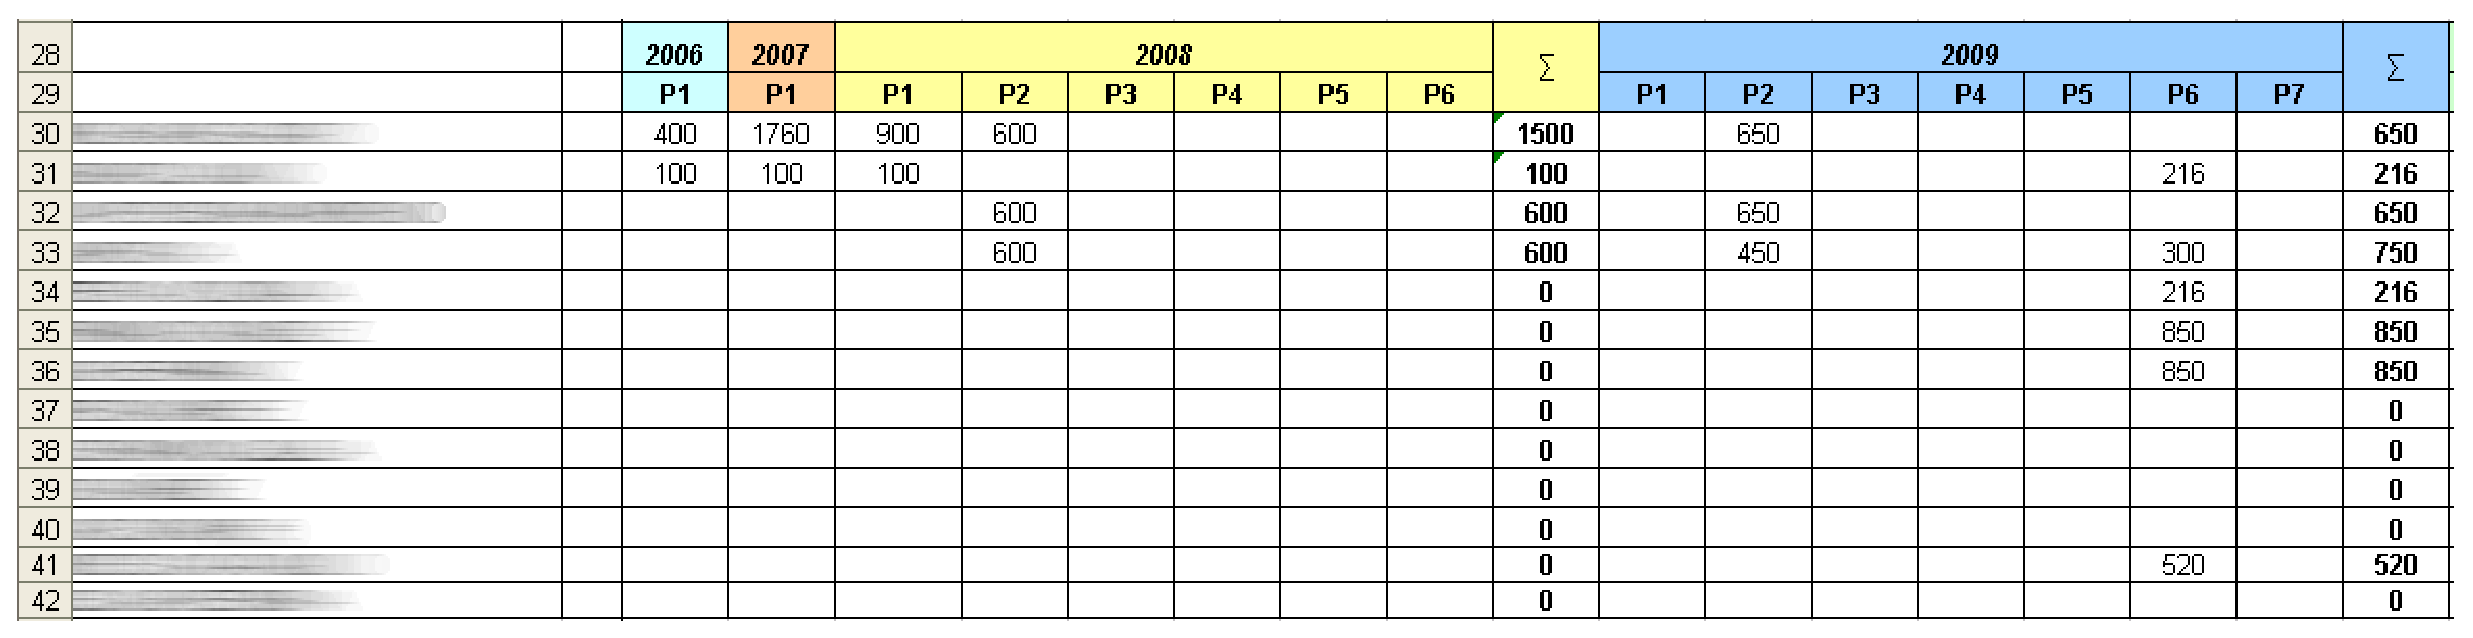
\epsfig{file=imagenes/registro.eps,width=5.28in}
\caption{Hoja de cálculo con el registro de horas asignadas.}
\label{fig:hoja_calculo}
\end{figure}

Por si no se aprecia adecuadamente en la imagen, las dos primeras columnas
coloreadas corresponden a un mismo proyecto en los años 2006 y 2007, y sólo
contienen datos de dos empleados. Las subdivisiones de la columna amarilla
corresponden a diversos proyectos cuyo desarrollo se extendía en el año 2008, y
de nuevo reflejan la carga de trabajo de cada empleado a lo largo del año
completo. Los datos son proporcionados por la empresa coordinadora del proyecto
y el objetivo de este registro no es otro que comprobar que no se están
imputando por error más horas a cada trabajador que las que tiene en su convenio
de trabajo. En este caso se está mostrando la tabla de horas justificadas, es
decir, horas que se llevaron a cabo una vez el proyecto estaba aprobado por los
organismos oficiales. Del mismo modo, existe una tabla para las horas
presentadas, ya que tampoco deberían proyectarse más horas de las que un
empleado puede llegar a trabajar.

Los problemas que se derivaban del uso de esta metodología eran diversos y de
difícil solución sin un rediseño completo de la metodología, a saber:
\begin{itemize}
\item la empresa cuenta con una base de datos de proyectos que no puede
contrastarse con la hoja de cálculo, de modo que debe comprobarse manualmente
el estado del proyecto para saber la naturaleza de las horas que deben ser
tenidas en cuenta;

\item no se guardaba registro de las horas del convenio colectivo, ni de la
fecha de alta o baja de los trabajadores, de manera que no podía asegurarse que
las horas imputadas no sobrepasaban las debidas;

\item el formato requería un alto grado de mantenimiento aun cuando no
contempla la nueva necesidad de especificar las horas por meses y actividades
individuales, en lugar de anualmente por proyectos. La nueva necesidad
simplemente era impracticable con el antiguo formato;

\item cualquier resumen de las horas asignadas que quisiera extraerse desde los
datos de la hoja de cálculo (por ejemplo: horas asignadas a un proyecto en
todos los años que abarca su desarrollo, horas asignadas a un empleado en
cualquiera de los proyectos en los que interviene...), debía elaborarse
manualmente por un trabajador cualificado, lo que consumía unos recursos que la
nueva herramienta reducirá al mínimo;

\item el antiguo formato tampoco guardaba registro del coste/hora de los
empleados, que varía, por lo general, anualmente, de modo que no se podía
calcular automáticamente el coste de los recursos humanos de los proyectos;

\item afinando un poco, es fácil deducir que no se puede llevar un registro de
proyectos en colaboración que, bien no duplique información ocasionando de nuevo
inconsistencias potenciales, bien no cause un aumento en el trabajo de
gestión: si tenemos varios clientes colaborando en un mismo proyecto debemos,
bien duplicar la información de los empleados para que figuren en las hojas de
cálculo de los otros clientes, bien consultar cada hoja de cálculo si
queremos extraer información acerca del proyecto en colaboración; 

\item a pesar de que podía detectarse cuándo se hizo la última modificación de
la hoja de cálculo, era imposible comprobar individualmente la actualidad de los
datos disponibles o quién los había modificado, lo que incrementaba el tiempo de
verificación de los datos cada vez que debían usarse para la creación de un
documento oficial.
\end{itemize}

\begin{table}
\centering
\begin{tabular}{|r|c|c|}\hline
 & hoja de cálculo & nueva herramienta \\\hline\hline
división mensual y por actividades &  \ding{55} &   \ding{51} \\\hline
verificación del límite de horas & \ding{55} &   \ding{51} \\\hline
bajo mantenimiento & \ding{55} &   \ding{51} \\\hline
informes automáticos & \ding{55} &   \ding{51} \\\hline
registro de coste/hora & \ding{55} &   \ding{51} \\\hline
fecha y responsable actualización & \ding{55} &   \ding{51} \\\hline
proyectos en colaboración & \ding{55} &   \ding{51} \\\hline
\end{tabular}
\caption{Listado de características principales.}
\end{table}

Adicionalmente, la nueva herramienta permitirá exportar algunos datos en formato
de hoja de cálculo, de manera que se conserva totalmente la funcionalidad
anterior.

% La figura \ref{fig:resumen_horas_asignadas_proyectos} corresponde a un resumen
% del mismo tipo utilizando la nueva herramienta:
% 
% \begin{figure}
% \centering
% 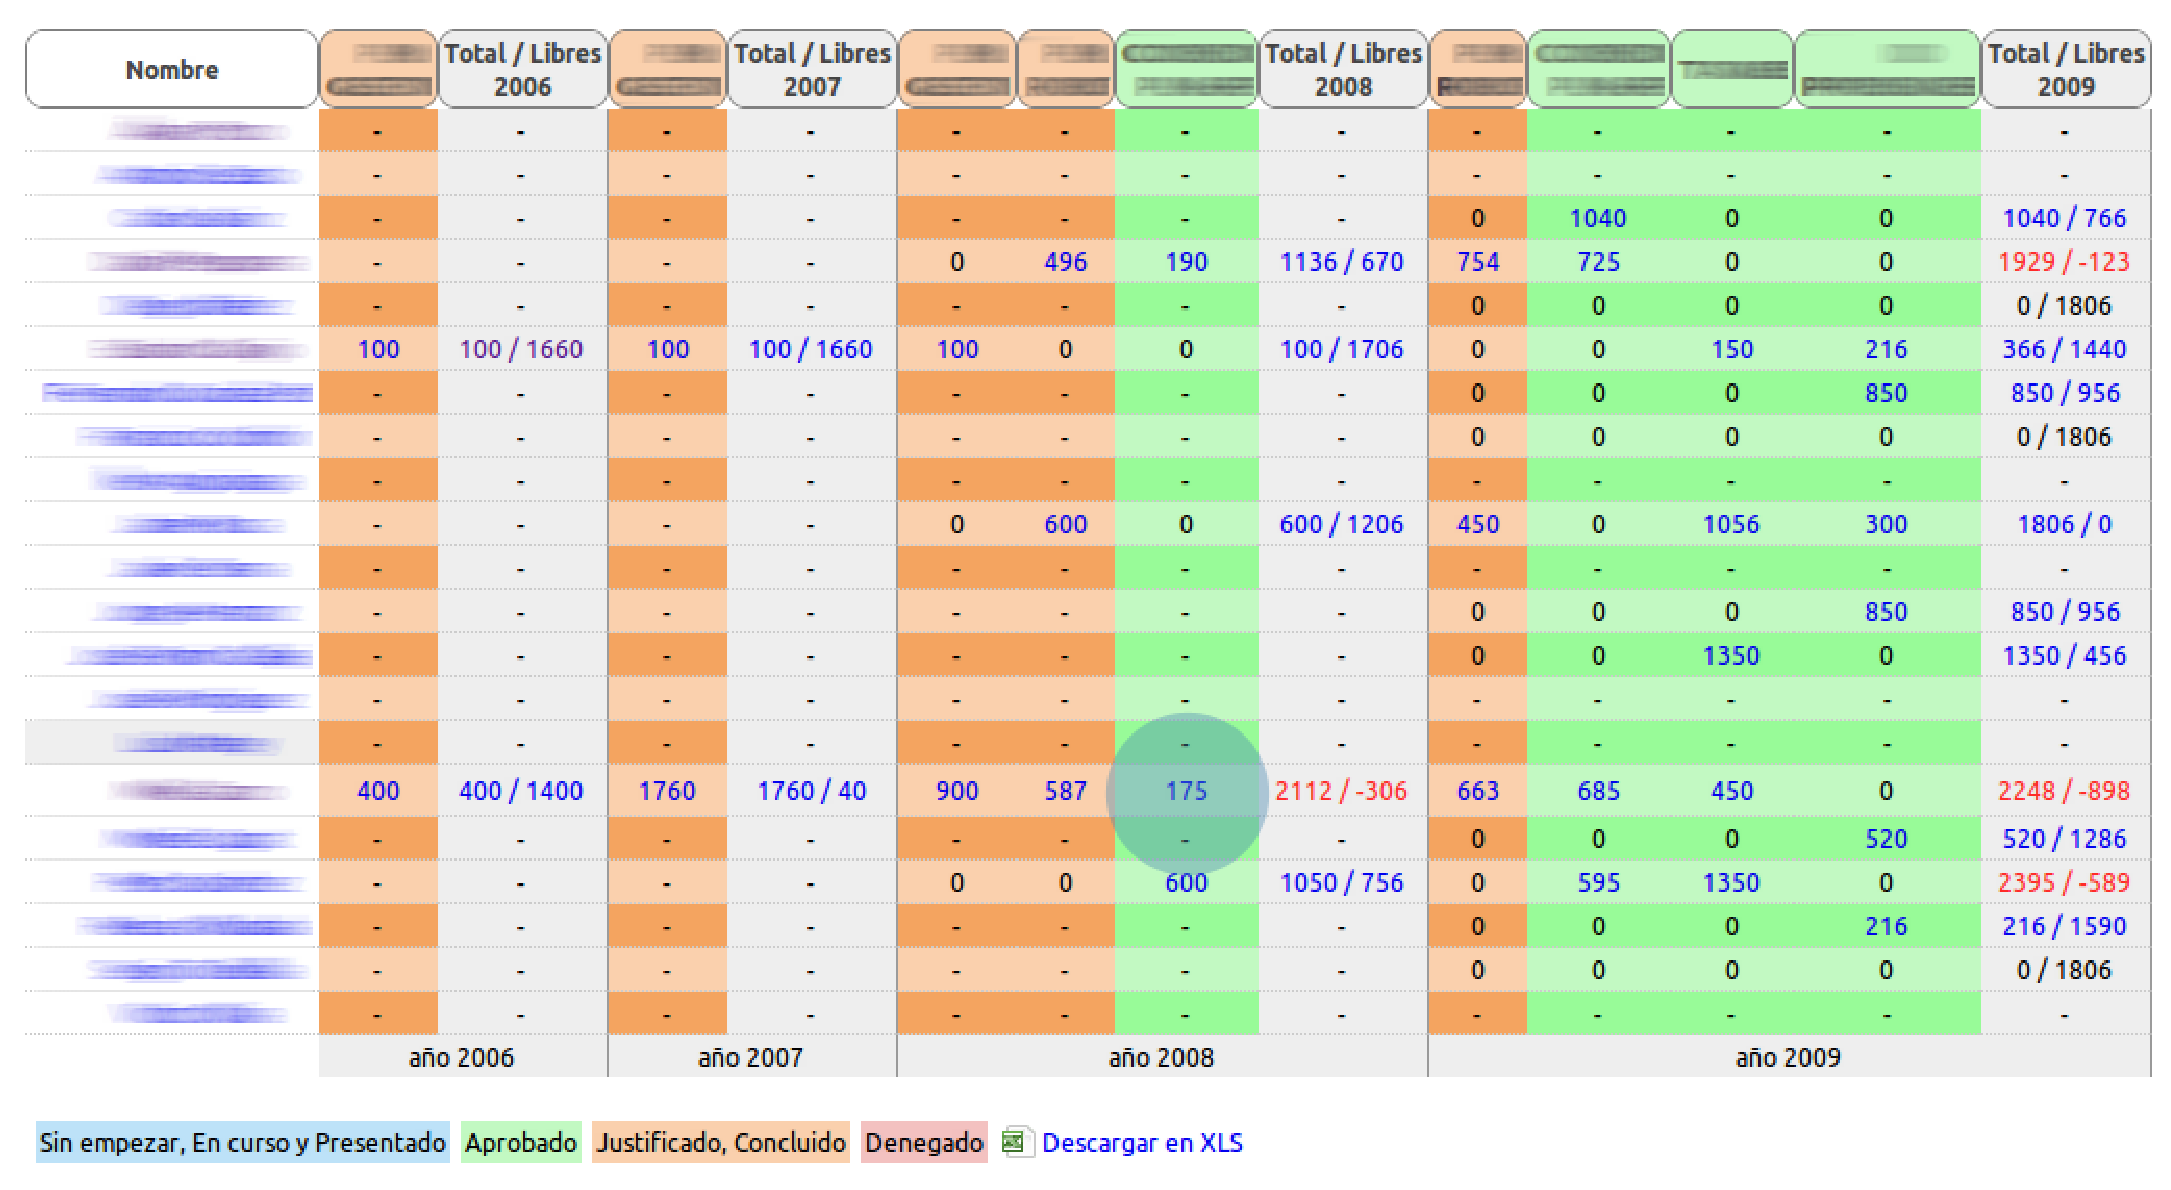
\epsfig{file=imagenes/prediccion_resumen2.eps,width=5.28in}
% \caption{Resumen de horas asignadas a proyectos.}
% \label{fig:resumen_horas_asignadas_proyectos}
% \end{figure}

De esta manera, la cantidad de información que se podrá extraer será
notablemente superior:

\begin{itemize}
\item podrá identificarse cuándo un empleado no estaba dado de alta en la
empresa.

\item se tendrá en cuenta el convenio de horas del recurso para informar acerca
de las horas que le quedan libres en un periodo;

\item cuando se produzca un conflicto, por ejemplo, se hayan imputado más horas
de las que deberían, el valor aparecerá marcado en rojo;

\item las columnas de proyectos seguirán un código de colores para indicar el
estado en que se encuentra el proyecto;

\item cada uno de los valores, incluidos los nombres de los recursos en
cuestión, serán un enlace a otra vista donde se darán detalles acerca
del elemento. Por ejemplo, pinchando en un valor de horas para un proyecto
determinado, obtendremos un desglose mensual y por actividades de esas horas con
un filtro en el que se podrán seleccionar tanto el empleado a visualizar, como
el año, mes, proyecto y actividad. La combinación de estos filtros creará una
flexibilidad sobresaliente a la hora de buscar la información que nos interesa
en cada momento. En esta vista, también se tendrá en cuenta el coste/hora de
cada empleado para calcular el coste de la selección.
\end{itemize}

% \begin{figure}
% \centering
% 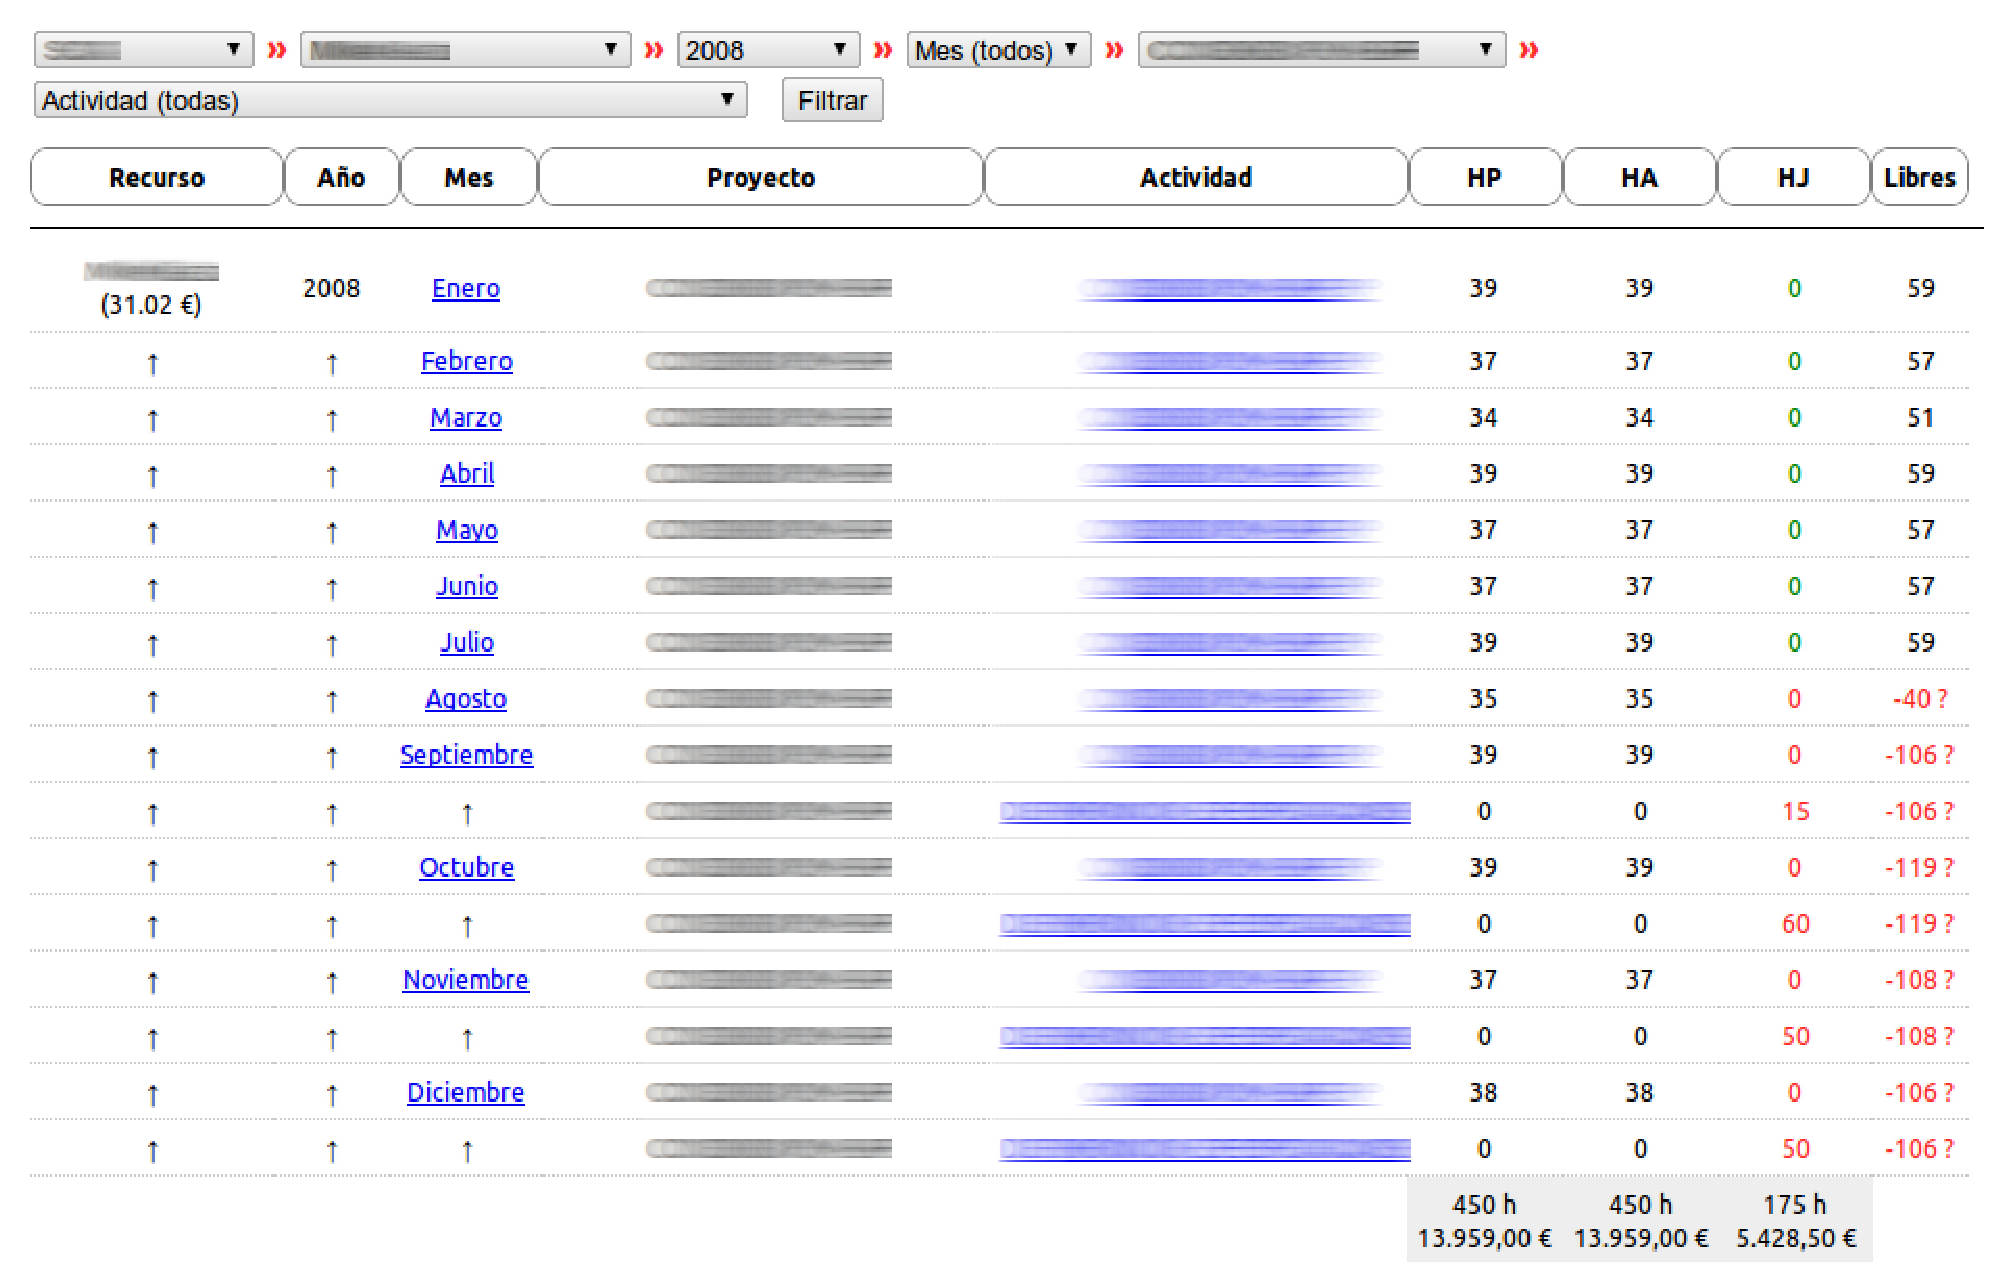
\epsfig{file=imagenes/desglose_mensual.eps,width=5.28in}
% \caption{Vista de desglose mensual por actividades.}
% \label{fig:desglose_mensual}
% \end{figure}

Revisiones muy simples de la distribución de horas del sistema antiguo han
mostrado que en casi la totalidad de los proyectos gestionados se produjo algún
tipo de inconsistencia: a veces dado
por las horas del convenio de los trabajadores y otras, porque a un
recurso se le estaban imputando horas de varios proyectos que
combinadas sobrepasaban el límite mensual supuesto un calendario laboral de 8
horas al día. Con la vista de desglose mensual de la nueva herramienta será muy
fácil filtrar la información para visualizar todas las horas imputadas (en
cualquier proyecto) a un empleado en los meses con inconsistencias.

En el supuesto de una auditoría por parte de los organismos públicos, estas
inconsistencias serían motivo suficiente para que un proyecto subvencionado por
cientos de miles de euros perdiera esa subvención.


\section{Acotación}
\label{sec:acotacion}

Una de las características que definen la aplicación es su respuesta a las
inconsistencias: como se explicó al inicio de la introducción, la herramienta
está pensada para \textit{dejar hacer} y detectar los errores, en lugar de
\textit{no dejar hacer} y proponer soluciones.

\begin{description}
 \item[Caso práctico] Supongamos que queremos grabar en la base de datos la
información del cuadro \ref{tab:distribucion_teorica} acerca de las horas que se
ha proyectado que Pepe Pérez
deberá trabajar en el desarrollo de dos proyectos:

\begin{table}
\centering
\begin{tabular}{|r|c|c||c|}\hline
 & horas proyecto 1  & horas proyecto 2 & total\\\hline\hline
septiembre 2010 & 90 & 110 & 200 \\\hline
octubre 2010 & 90 & 50 & 140\\\hline\hline
total & 180 & 160 & 340\\\hline
\end{tabular}
\caption{Distribución teórica de Pepe Pérez.}
\label{tab:distribucion_teorica}
\end{table}

La inconsistencia se va a dar porque septiembre de 2010 tuvo 22 días laborables,
que se corresponden con 176 horas de trabajo, lejos de las 200 que se están
intentando imputar. Un sistema relativamente avanzado completaría el mes de
septiembre hasta los límites máximos y traspasaría las horas restantes al
siguiente mes, como se muestra en el cuadro \ref{tab:distribucion_ideal}.

\begin{table}
\centering
\begin{tabular}{|r|c|c||c|}\hline
 & horas proyecto 1  & horas proyecto 2 & total \\\hline\hline
septiembre 2010 & 90 & 86 & 176 \\\hline
octubre 2010 & 90 & 74 & 164\\\hline\hline
total & 180 & 160 & 340\\\hline
\end{tabular}
\caption{Distribución ideal de Pepe Pérez.}
\label{tab:distribucion_ideal}
\end{table}

De esta manera, septiembre estaría completo y octubre tendría un total de 164
horas, 4 por debajo del límite mensual marcado por los 21 días laborables que
tuvo ese mes. La inconsistencia habría desaparecido y se habría logrado
conservar el total de horas proyectadas. Sin embargo, esto no siempre va a ser
posible y en el caso que nos ocupa, al tratarse de proyectos de terceros, se
depende de la información que ellos proporcionen y debe grabarse tal cual
llega. Con esta premisa, lo máximo que se puede hacer es informar de la
naturaleza de la inconsistencia para que un técnico busque la solución más
adecuada (véase el cuadro \ref{tab:distribucion_marcada}).

\begin{table}
\centering
\begin{tabular}{|r|c|c||c|}\hline
 & horas proyecto 1  & horas proyecto 2 & total\\\hline\hline
septiembre 2010 & 90 & 110 & {\color{red} 200(-24)} \\\hline
octubre 2010 & 90 & 50 & 140\\\hline\hline
total & 180 & 160 & 340\\\hline
\end{tabular}
\caption{Distribución teórica con marcado de inconsistencias.}
\label{tab:distribucion_marcada}
\end{table}

\end{description}

Hay que recordar que el objetivo de la aplicación se refiere más a la auditoría
de datos y generación de informes que a la de planificación como tal. Esto se
debe, como se ha indicado en el párrafo anterior, a la dependencia de
información externa. La aplicación, sin embargo, sí cuenta con funciones
dedicadas que se emplearán a la hora de planificar proyectos internos de
Ingeniería e Innovación.




\chapter{Descripción general del proyecto}
\label{chp:descripcion}
\thispagestyle{empty}
\noindent \textit{En este capítulo se detallarán los elementos más generales
en relación con el proyecto, desde los interesados, el objetivo, las
tecnologías que se emplearán y otros hechos relevantes.}
\section{Propósito del proyecto}

\subsection{Contexto}

La aplicación se enmarca en el contexto de la gestión de recursos en el ámbito
empresarial. En este caso, la aplicación no tiene un objetivo comercial, será
usada solamente por los empleados de Ingeniería e Innovación.

\subsection{Objetivo general}

El objetivo es desarrollar una herramienta de fácil uso para que los empleados
de Ingeniería e Innovación puedan llevar un registro detallado de los recursos
humanos empleados en los proyectos que gestionan.

\section{El cliente y otros interesados}

\subsection{El cliente}

El único cliente es Ingeniería e Innovación.

\subsection{Otros interesados}

\begin{itemize}
 \item Desarrollador: en este caso, el proyectante, Javier Cejudo, se encarga
de todos los aspectos relacionados con el desarrollo del sistema desde sus
primeras etapas hasta la finalización del mismo.

\item Tutor: Ángel Luis Rubio, se encarga de la orientación del proyecto para
que se adecue a lo que debe ser un PFC.

\item Tutor de empresa: León Arnedo, es en cierto modo el principal
representante del cliente, pero también se encarga de la orientación del
proyecto para que se adecue a sus necesidades.
Es también el principal \textit{testeador} de la aplicación.
\end{itemize}


\section{Los usuarios del producto}

\subsection{Usuarios finales}

\begin{itemize}
 \item Los empleados de la empresa: todos tienen amplia
experiencia en el uso de sistemas de información. De hecho, la herramienta a
desarrollar en este proyecto se integrará en una intranet de uso común a todos
los empleados.

\item Usuarios de mantenimiento: el mantenimiento será llevado a cabo por
alguno de los empleados de la empresa con conocimientos de PHP. Todos son
ingenieros industriales sin amplia experiencia en el tema.
\end{itemize}

\subsection{Prioridades asignadas a los usuarios}

Por la naturaleza del sistema, y ya que no se prevé que vayan a
ser necesarias ampliaciones considerables, los usuarios finales serán la
prioridad a la hora de diseñar el producto; los usuarios de mantenimiento se
encargarían de solucionar problemas potenciales o realizar cambios mínimos.

\section{Tecnologías a utilizar}
\label{sec:tecnologias}

La decisión acerca de las tecnologías a utilizar se ha basado casi
exclusivamente en los requisitos de Ingeniería e Innovación. La arquitectura
básica de la aplicación (la de la empresa puede verse en la figura
\ref{fig:arquitectura_iandi}) consiste en un servidor ejecutando sobre Microsoft
Windows con una base de datos MySQL interpretada en el lado del servidor
mediante PHP, cuyo código resultante es gestionado por el servidor web HTTP
Apache. La nueva funcionalidad que proporciona el desarrollo de este proyecto
debía integrarse de forma consistente, de manera que esas serán las tecnologías
que soporten el desarrollo del proyecto.

\begin{figure}
\centering
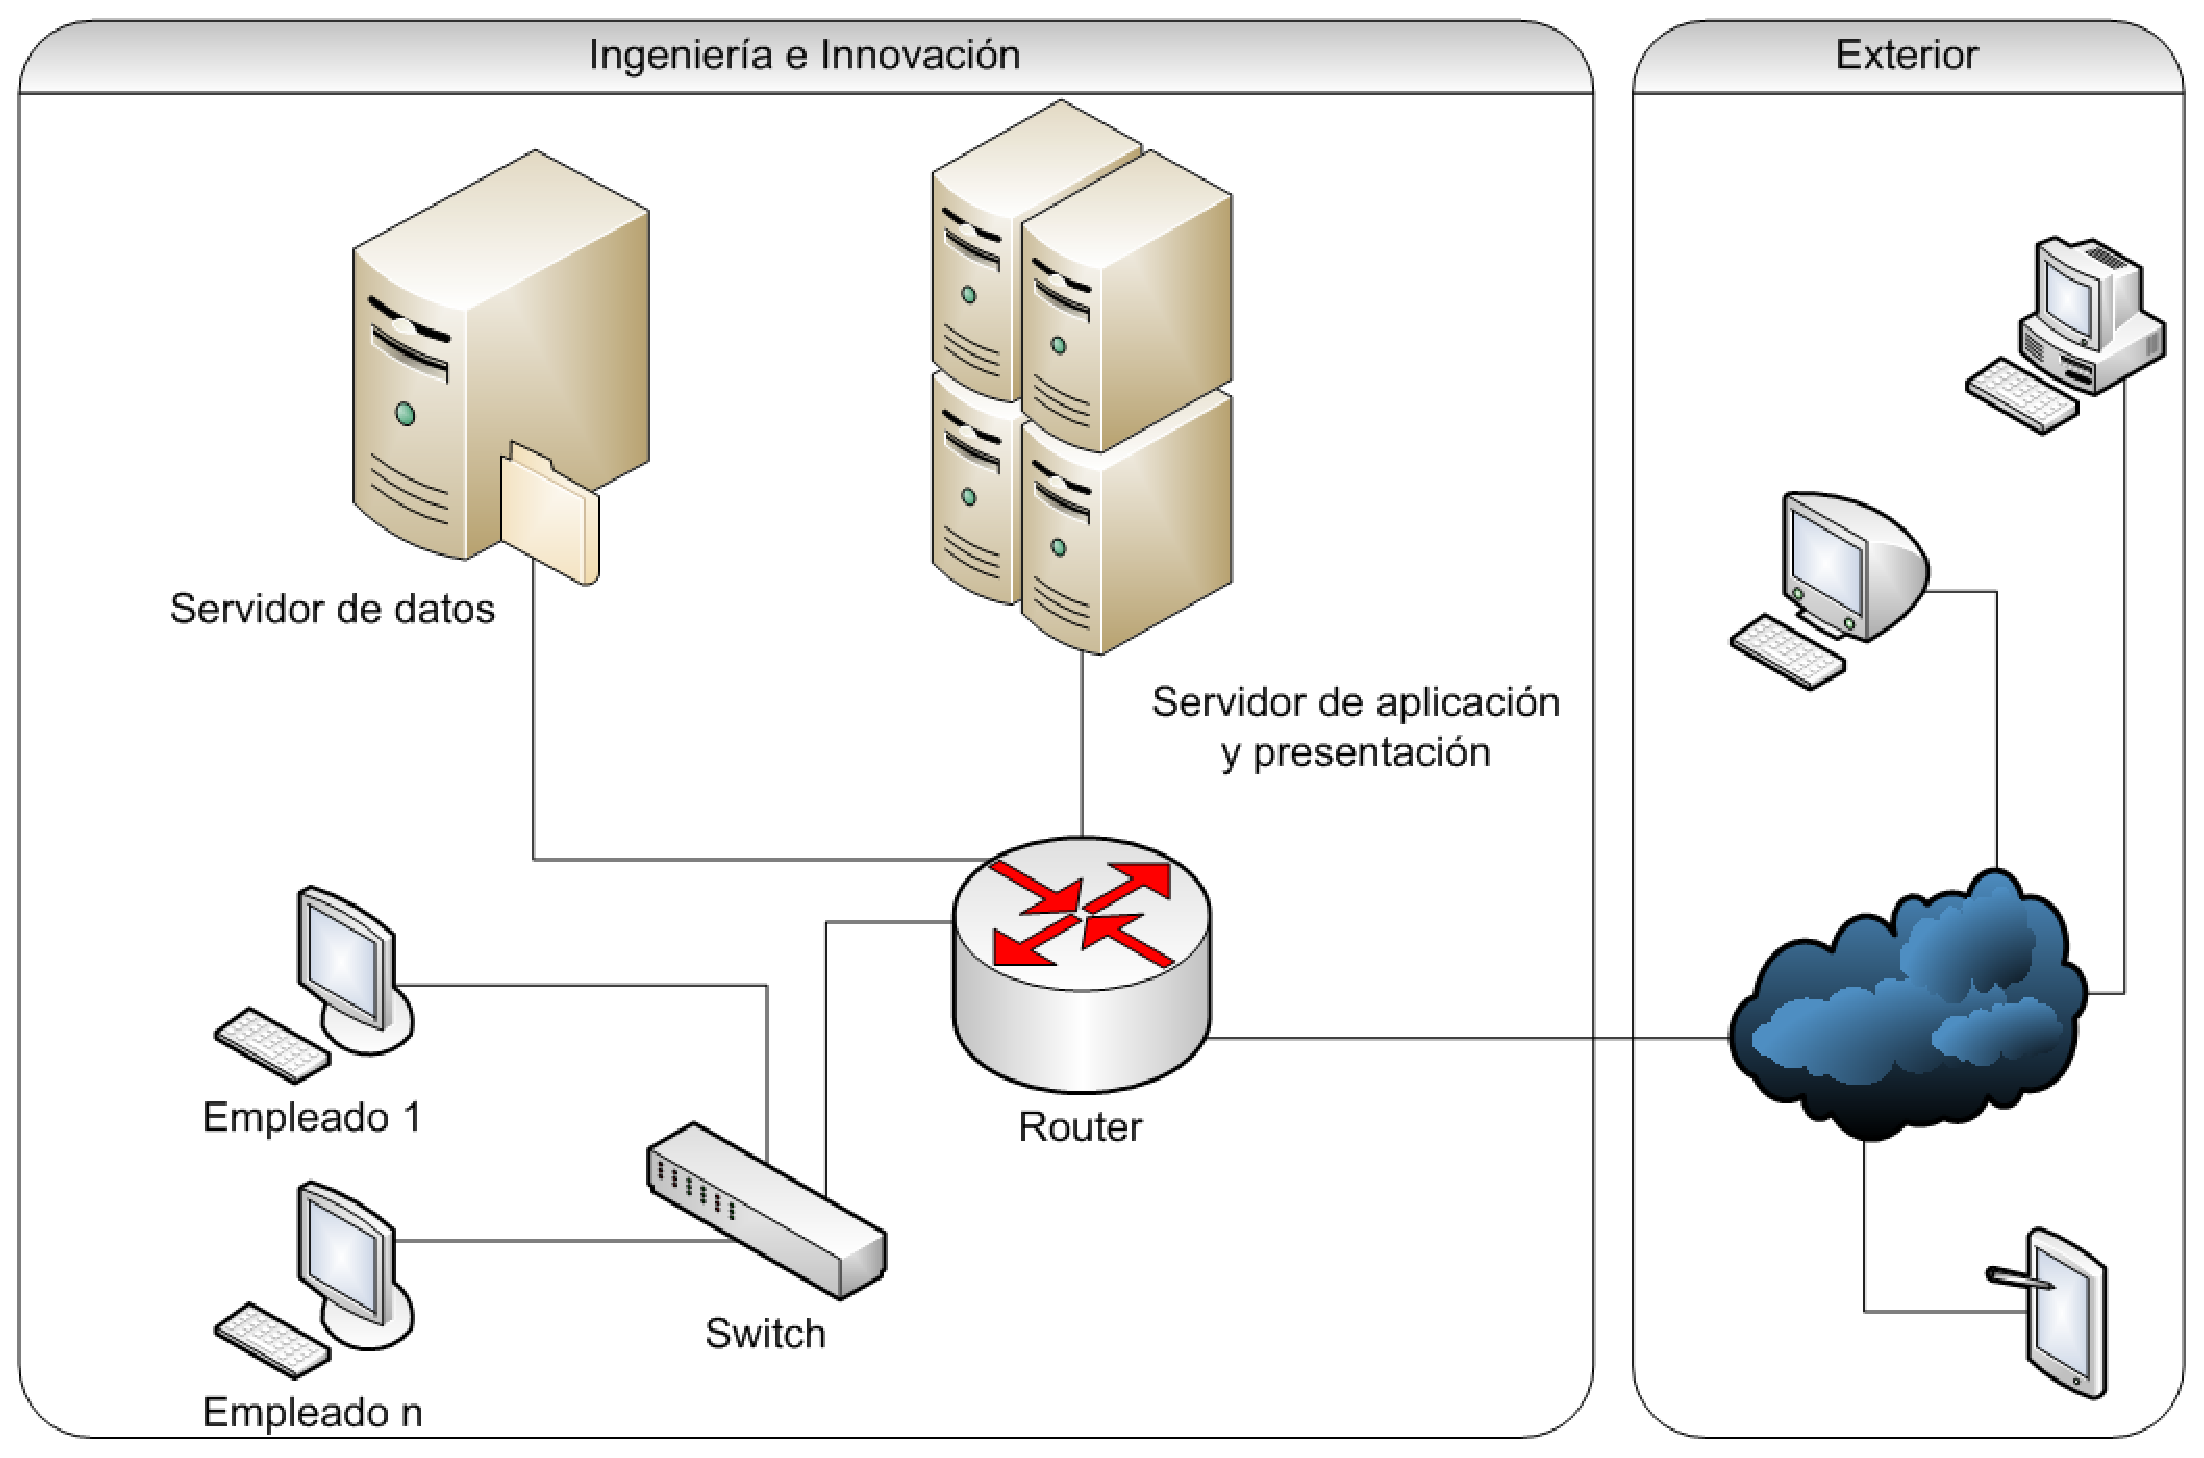
\epsfig{file=imagenes/arquitectura_iandi.eps,width=5.28in}
\caption{Arquitectura hardware de la empresa.}
\label{fig:arquitectura_iandi}
\end{figure}

En el plano de la programación, y a pesar de que PHP ofrece el paradigma de
orientación a objetos desde su versión 3 (Junio de 1998), se ha optado por
seguir con el paradigma imperativo presente en el resto de la aplicación.

\subsection{Alternativas de implementación}

Las alternativas a la implementación son numerosas, pero ninguna de ellas
resultaba razonable dadas las características descritas en los párrafos
anteriores:

\begin{itemize}
\item Podrían haberse empleado otros lenguajes de programación del lado del
servidor, desde Perl, Python, Ruby... e incluso la tecnología ASP, aunque
en este último caso debería haberse pasado a usar IIS como servidor web;

\item Comprendiendo las ventajas que ofrece la programación orientada a objetos,
el proyectante se planteó realizar los nuevos módulos usando este paradigma,
pero la posibilidad se descartó debido a la fuerte dependencia del sistema con
conceptos previamente tratados de forma imperativa. Un cambio en este sentido
habría supuesto la convivencia de dos modelos diferenciados o la definición de
clases para el tratamiento de unos objetos que si bien interactúan con la nueva
funcionalidad, no forman parte del marco de desarrollo de este proyecto.
\end{itemize}

Además, una vez que el proyectante finalizase su labor en la empresa, el sistema
sería mantenido por ingenieros industriales con conocimientos de PHP pero sin
la formación básica de orientación a objetos.

\section{Hechos relevantes y asunciones}

\subsection{Hechos}

\begin{itemize}
 \item La interfaz será desarrollada siguiendo las especificaciones HTML 4.01 y
CSS2, ya que es la manera en que está desarrollado el resto de la aplicación,
sin perjuicio de incluir puntualmente funcionalidades de HTML5 y CSS3.
\item La aplicación estará instalada en un servidor de Ingeniería e Innovación
\item Debe estar disponible 24 horas al día, 7 días a la semana.
\end{itemize}

Un hecho que merece mención aparte es que el proyecto no es independiente, es
decir, forma parte de un sistema mayor en uso. De esta manera, es necesario que
se adapte de la forma más \textit{suave} posible a aquel sistema. Para ello, se
estudió en profundidad su funcionamiento y se adoptaron todas las convenciones
que fue posible, desde la forma que el sistema existente tenía de almacenar
fechas en la base de datos, hasta los métodos para comprobar en cada página que
un usuario está autenticado.

\subsection{Asunciones}

\begin{itemize}
\item El usuario usa un ordenador de escritorio con un navegador web. Otros
dispositivos (p. ej.:móviles) no están soportados.
\item El usuario no tiene problemas graves de accesibilidad. El desarrollo no
se centrará en la accesibilidad del producto más allá de seguir las
recomendaciones de las especificaciones HTML 4.01 y CSS2.
\item En general, la herramienta se utilizará de manera local en las
instalaciones del cliente, pero el portal web permite acceso a la intranet
desde el exterior (extranet), por lo que el rendimiento de la herramienta debe
estar adaptado a esta característica.
\end{itemize}

\section{Aspectos relativos a los usuarios dentro del sistema}
\label{sec:usuarios_del_sistema}

La aplicación, tal y como se encontraba al inicio de este proyecto, contaba con
dos tipos de usuarios: usuario básico y Administrador.

\subsection{Usuario básico}
\label{sec:usuario_basico}

Todos los miembros de la empresa tienen un usuario creado en la base de datos
que les permite gestionar temas relativos a proyectos, expedientes,
facturación... La información es común a todos los miembros de la organización,
y el único control que se lleva a cabo es el registro de cuándo y quién realizó
la última actualización de los datos. La organización es los suficientemente
pequeña para que este sistema haya permitido durante al menos dos años de
existencia de la aplicación, una gestión más ágil sin provocar errores o
inconsistencias notables.

\subsection{Administrador}
\label{sec:administrador}

El Administrador puede dar de alta/baja usuarios y realizar operaciones
delicadas relativas a la modificación de datos considerados estáticos (no
deberían cambiar a lo largo del tiempo, pero pueden haberse introducido
erróneamente), y al borrado de datos de la base de datos, que siempre ha de
meditarse y valorarse detenidamente.

En los nuevos módulos desarrollados por el proyectante se ha mantenido la
misma metodología. Si bien se planteó la posibilidad de que el acceso a
determinados datos (facturas, proyectos, etc.), solamente estuviera autorizado
según qué usuario intentase acceder, esta posibilidad se desestimó, de nuevo,
debido al pequeño tamaño de la organización y al buen resultado que ha tenido un
sistema más abierto.

También se planteó la posibilidad de abrir la aplicación a los clientes
externos, de manera que ellos mismos pudieran introducir los datos de horas
trabajadas por sus empleados en lugar de tener que proporcionar esa información
a Ingeniería e Innovación y que fuera un empleado de ésta última quien
finalmente grabase los datos. Este sistema ahorraría un paso en el proceso y
los errores que se pudieran derivar de ello; sin embargo, y por motivos de
seguridad, se decidió que la apertura de la aplicación se aplazaría hasta
futuros ciclos de desarrollo.

\chapter{Calendario}
\label{chp:calendario}
\thispagestyle{empty}
\noindent \textit{Este capítulo supone un repaso al calendario de ejecución
real del proyecto desde los primeros contactos con el cliente hasta la
preparación y entrega de esta memoria, con una breve explicación de cada fase
de desarrollo.}
Como se indicó en la introducción de esta memoria, el proyectante comenzó las
labores de ejecución del proyecto durante unas prácticas de empresa, antes de
decidir que se convertiría en su Proyecto Fin de Carrera. Es por ello que no se
hizo un \textit{Documento de Objetivos del Proyecto} ni un \textit{Plan de
Trabajo}.

En cambio, sí ha sido posible documentar con detalle cuál fue la evolución del
desarrollo del proyecto ya que, siguiendo la metodología de la empresa en la
que se realizó el desarrollo, se llevaba un registro diario de las actividades
realizadas.

El calendario se ha dividido en varias partes, siguiendo el proceso de trabajo
dividiéndolo en varias fases. Puede apreciarse que hay un periodo de
inactividad entre enero y febrero de 2011, entre la clasifcación de
\textit{bugs}, sugerencias... y la última recodificación. Este periodo
pertenece a una indisponibilidad por motivos familiares que, por suerte, no ha
resultado en retrasos con consecuencias mayores.

A continuación se describen de forma básica las acciones realizadas
por el proyectante en cada fase de desarrollo desde de que este comenzase allá
por junio de 2010 hasta que se depositó finalmente en junio de 2011. 

\section{Dirección del proyecto}

Se han incluido en esta sección todas las
actividades relacionadas con la comunicación con el cliente y el tutor del
proyecto.

\subsection{Comunicación con el cliente}

La primera reunión con el cliente para tratar específicamente el desarrollo de
este proyecto se llevó a cabo el 18 de junio de 2010, cuando el proyectante
llevaba realizando prácticas en la empresa un mes exactamente. Se trató la
necesidad del cliente, detallada en la sección \ref{sec:necesidad} (página
\pageref{sec:necesidad}), pero no la posibilidad de que esas labores se
convirtieran en su PFC.
La comunicación con el cliente ha sido constante a lo largo de todo el
proyecto, una característica que ha hecho posible que tanto desde el punto de
vista del proyectante como del cliente, el proyecto haya sido un éxito. Si
bien, al contrario de como se debía, no se elaboraron documentos específicos
acerca de la planificación, análisis... de cada parte, estos fueron sustituidos
por una comunicación constante, prácticamente diaria, con el cliente, que ha
supervisado la evolución del proyecto cada vez que su avance permitía ver
nuevos resultados o realizar nuevas pruebas. Cualquier no conformidad se
resolvía, con esta metodología, de manera casi inmediata, de manera que las
replanificaciones han sido, con alguna excepción no trivial, mínimas.

\subsection{Comunicación con el tutor}

Los primeros contactos con Ángel Luis Rubio, tutor de este proyecto, se
llevaron a cabo en septiembre de 2010 vía correo electrónico, y culminaron con
una primera reunión el 25 de octubre en la que se revisó lo hecho hasta el
momento y se concluyó que el reto que planteaba el desarrollo del proyecto
era adecuado como PFC, ni demasiado simple ni demasiado complejo.

Posteriormente, el contacto continuó a través de correo electrónico, con otra
reunión presencial el 11 de abril para resolver algunas dudas del proyectante
acerca de la organización y elaboración de la presente memoria.

\section{Módulo de personal}

Sin ánimo de adelantar detalles que corresponden a los próximos capítulos,
el módulo de personal fue la primera parte que se desarrolló. Se completó antes
de iniciar cualquier tipo de análisis de los módulos subsiguientes. La razón,
en un primer momento, era que el cliente pudiera confirmar la habilidad del
proyectante para completar un proyecto del alcance que ha llegado a tener. Así,
se llevó a cabo un gestor de personal cuyo funcionamiento interno se integra
apropiadamente con la base de datos existente y que es capaz de realizar todas
las funciones que necesitaba el cliente.

Este desarrollo se extendió desde la primera reunión con el cliente, en junio
de 2010, hasta mediados de agosto, en ratos libres dentro de las horas de
prácticas de empresa. La secuencia de actividades puede verse en el diagrama de
Gantt al final de este capítulo.

En resumen, las especificaciones principales
se definieron en una primera reunión con el cliente, a la que siguió un
esfuerzo por parte del proyectante de detección de entidades y diseño de la
base de datos que serviría de soporte lógico de almacenamiento de los datos.
Posteriormente, otra vez de acuerdo con el cliente, se realizaron una serie de
bocetos para la interfaz de usuario que se concretarían con el marcado HTML y
CSS, para continuar con la codificación de las funciones relativas a la gestión
del personal.

Una vez completado el desarrollo, el cliente revisaría el módulo para confirmar
que cumplía las especificaciones, y todo el \textit{feedback} sirvió para
mejorar la experiencia del usuario en una última fase de recodificación que,
por que el lector se haga una idea, añadió pequeños detalles como la posibilidad
de que al añadir datos anuales a un empleado, se tomasen por defecto los datos
del año anterior.

\section{Módulo de actividades}

Con un concepto similar al módulo de personal, se completó el
gestor de actividades antes de plantear la última fase de desarrollo
propiamente dicho. Así, siguiendo el mismo esquema de actividades que en la
sección anterior, las labores se extendieron desde mediados de agosto de
2010 hasta finales de septiembre.

Debe aclararse que la adición de la gestión de horas exige algunas pequeñas
modificaciones en la forma en que se presentan los datos relacionados con el
personal y las actividades, pero esas labores se han incluido en la siguiente
fase, no como recodificaciones de las mismas.

\section{Módulo de gestión de horas e integración}

Esta última parte del desarrollo fue la más complicada, pero gracias a la
experiencia adquirida en las fases anteriores, fue posible completarla con un
esquema de tiempos similar. Incluye la integración de todas las partes, ya que
a pesar de haber realizado desarrollos separados, las tres están íntimamente
relacionadas.

\section{Buscador global}

El buscador se desarrolló de forma más independiente, ya que fue una propuesta
del proyectante. Su desarrollo se llevó a cabo en ratos libres durante un
periodo de tres semanas, una vez se hubo implementado el módulo de personal.
Lo único que se añadió a posteriori fue un enlace de interés a las actividades
de los clientes y los proyectos, que son las dos entidades que se pueden
buscar, junto con los recursos. De cualquier modo, los detalles acerca del
buscador se pueden consultar en las secciones correspondientes de la presente
memoria.

\section{Última recodificación}

Apenas un mes después de que la herramienta comenzase a utilizarse en casos
reales y actuales y se hubieran reunido algunas sugerencias de modificación,
el proyectante sufrió una indisponibilidad familiar entre enero y febrero de
2011, periodo durante el cual cesó cualquier actividad del proyectante en
relación con la herramienta. Sin embargo, Ingeniería e Innovación siguió
utilizando el sistema sin mayores problemas y las mejoras que surgieron, todas
menores --más acerca de la usabilidad que de la funcionalidad--, fueron
implementadas en esta última etapa de codificación, que incluyó,
principalmente, hacer visible más resúmenes de los datos que ya estaban en la
base de datos y corregir algunos detalles relativos a la colaboración de
clientes en proyectos.

\section{Memoria y defensa}

Esta memoria comenzó a escribirse a mediados de abril del 2010, con la fecha de
finalización que aparece en la portada (el límite para su depósito fue el 17 de
junio). Como se ha indicado anteriormente, la forma en que se ha llevado a cabo
una vez finalizada la parte técnica del proyecto.

Por su parte, la fecha prevista para el inicio de la preparación para la
presentación y defensa del proyecto es mediados de junio, una vez finalizada
esta memoria completamente.

\begin{figure}[h]
\centering
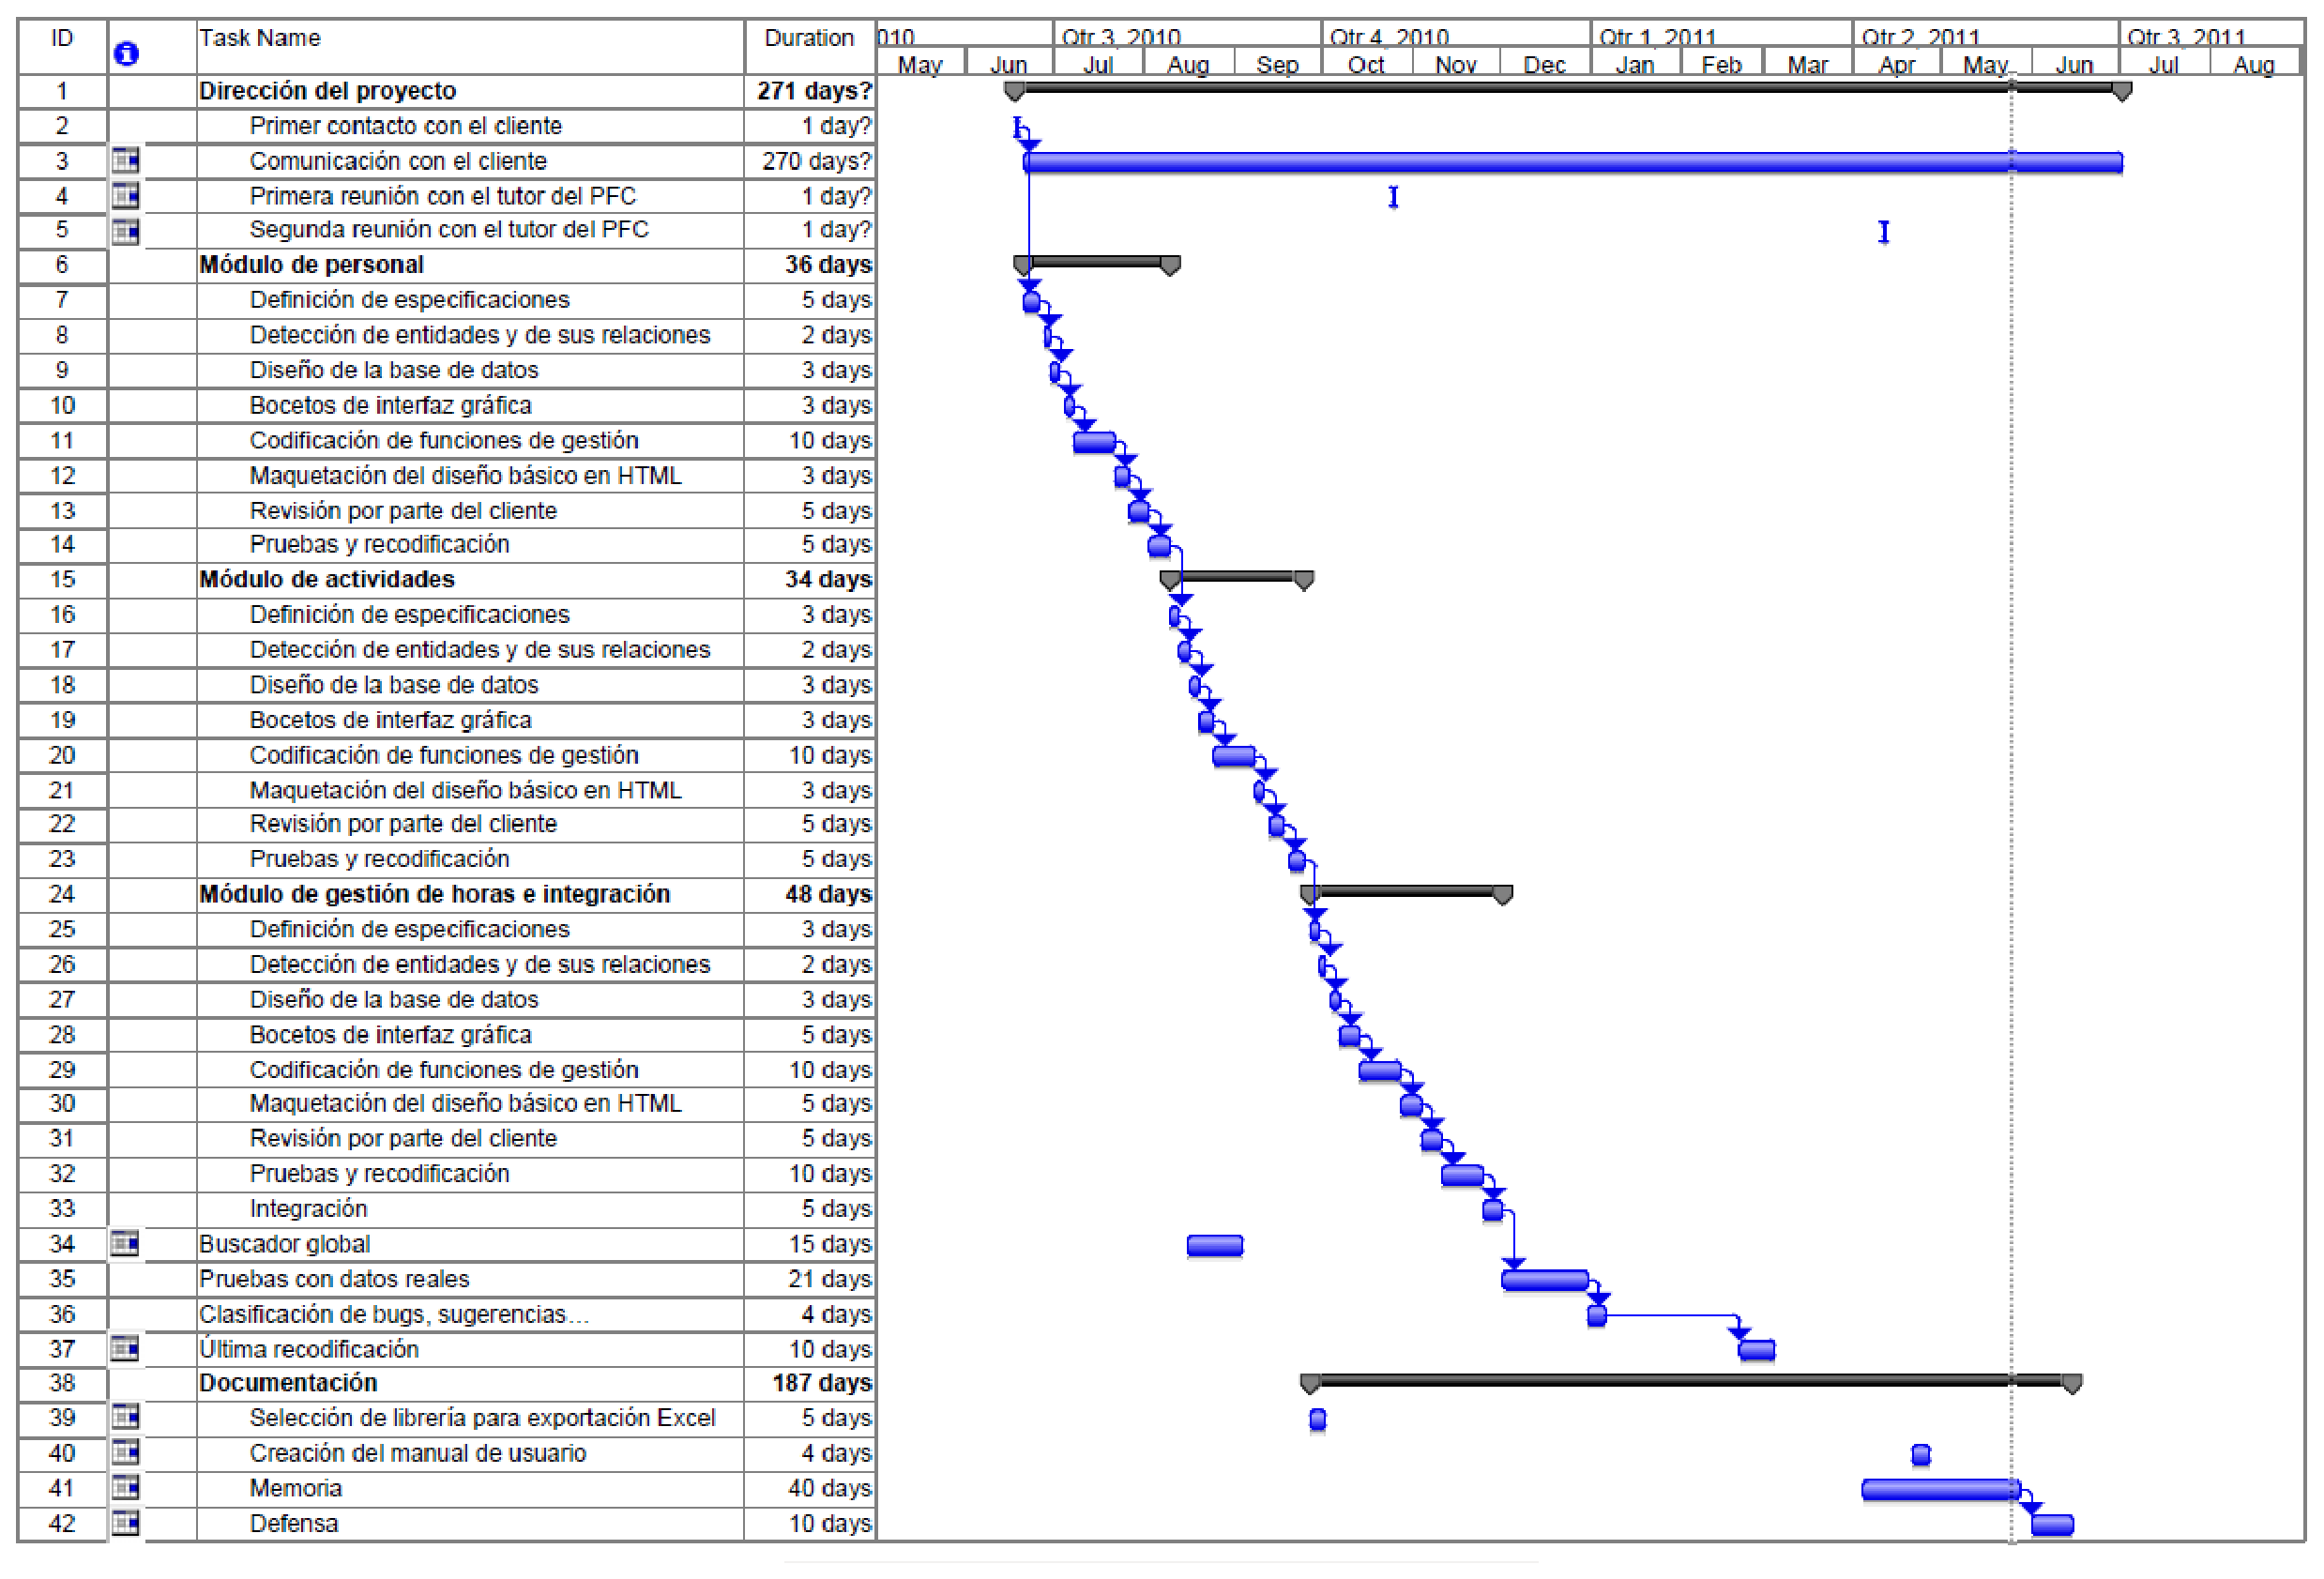
\epsfig{file=imagenes/gantt.eps,width=5.28in}
\caption{Diagrama de Gantt.}
\label{fig:gantt}
\end{figure}

%%%%GANTT
% {\linespread{1} \vfill\newpage
% \newsavebox{\myboxa}
% \sbox{\myboxa}{
% \begin{minipage}[t]{\textheight}
% \quad \vspace*{10pt}
% 
% 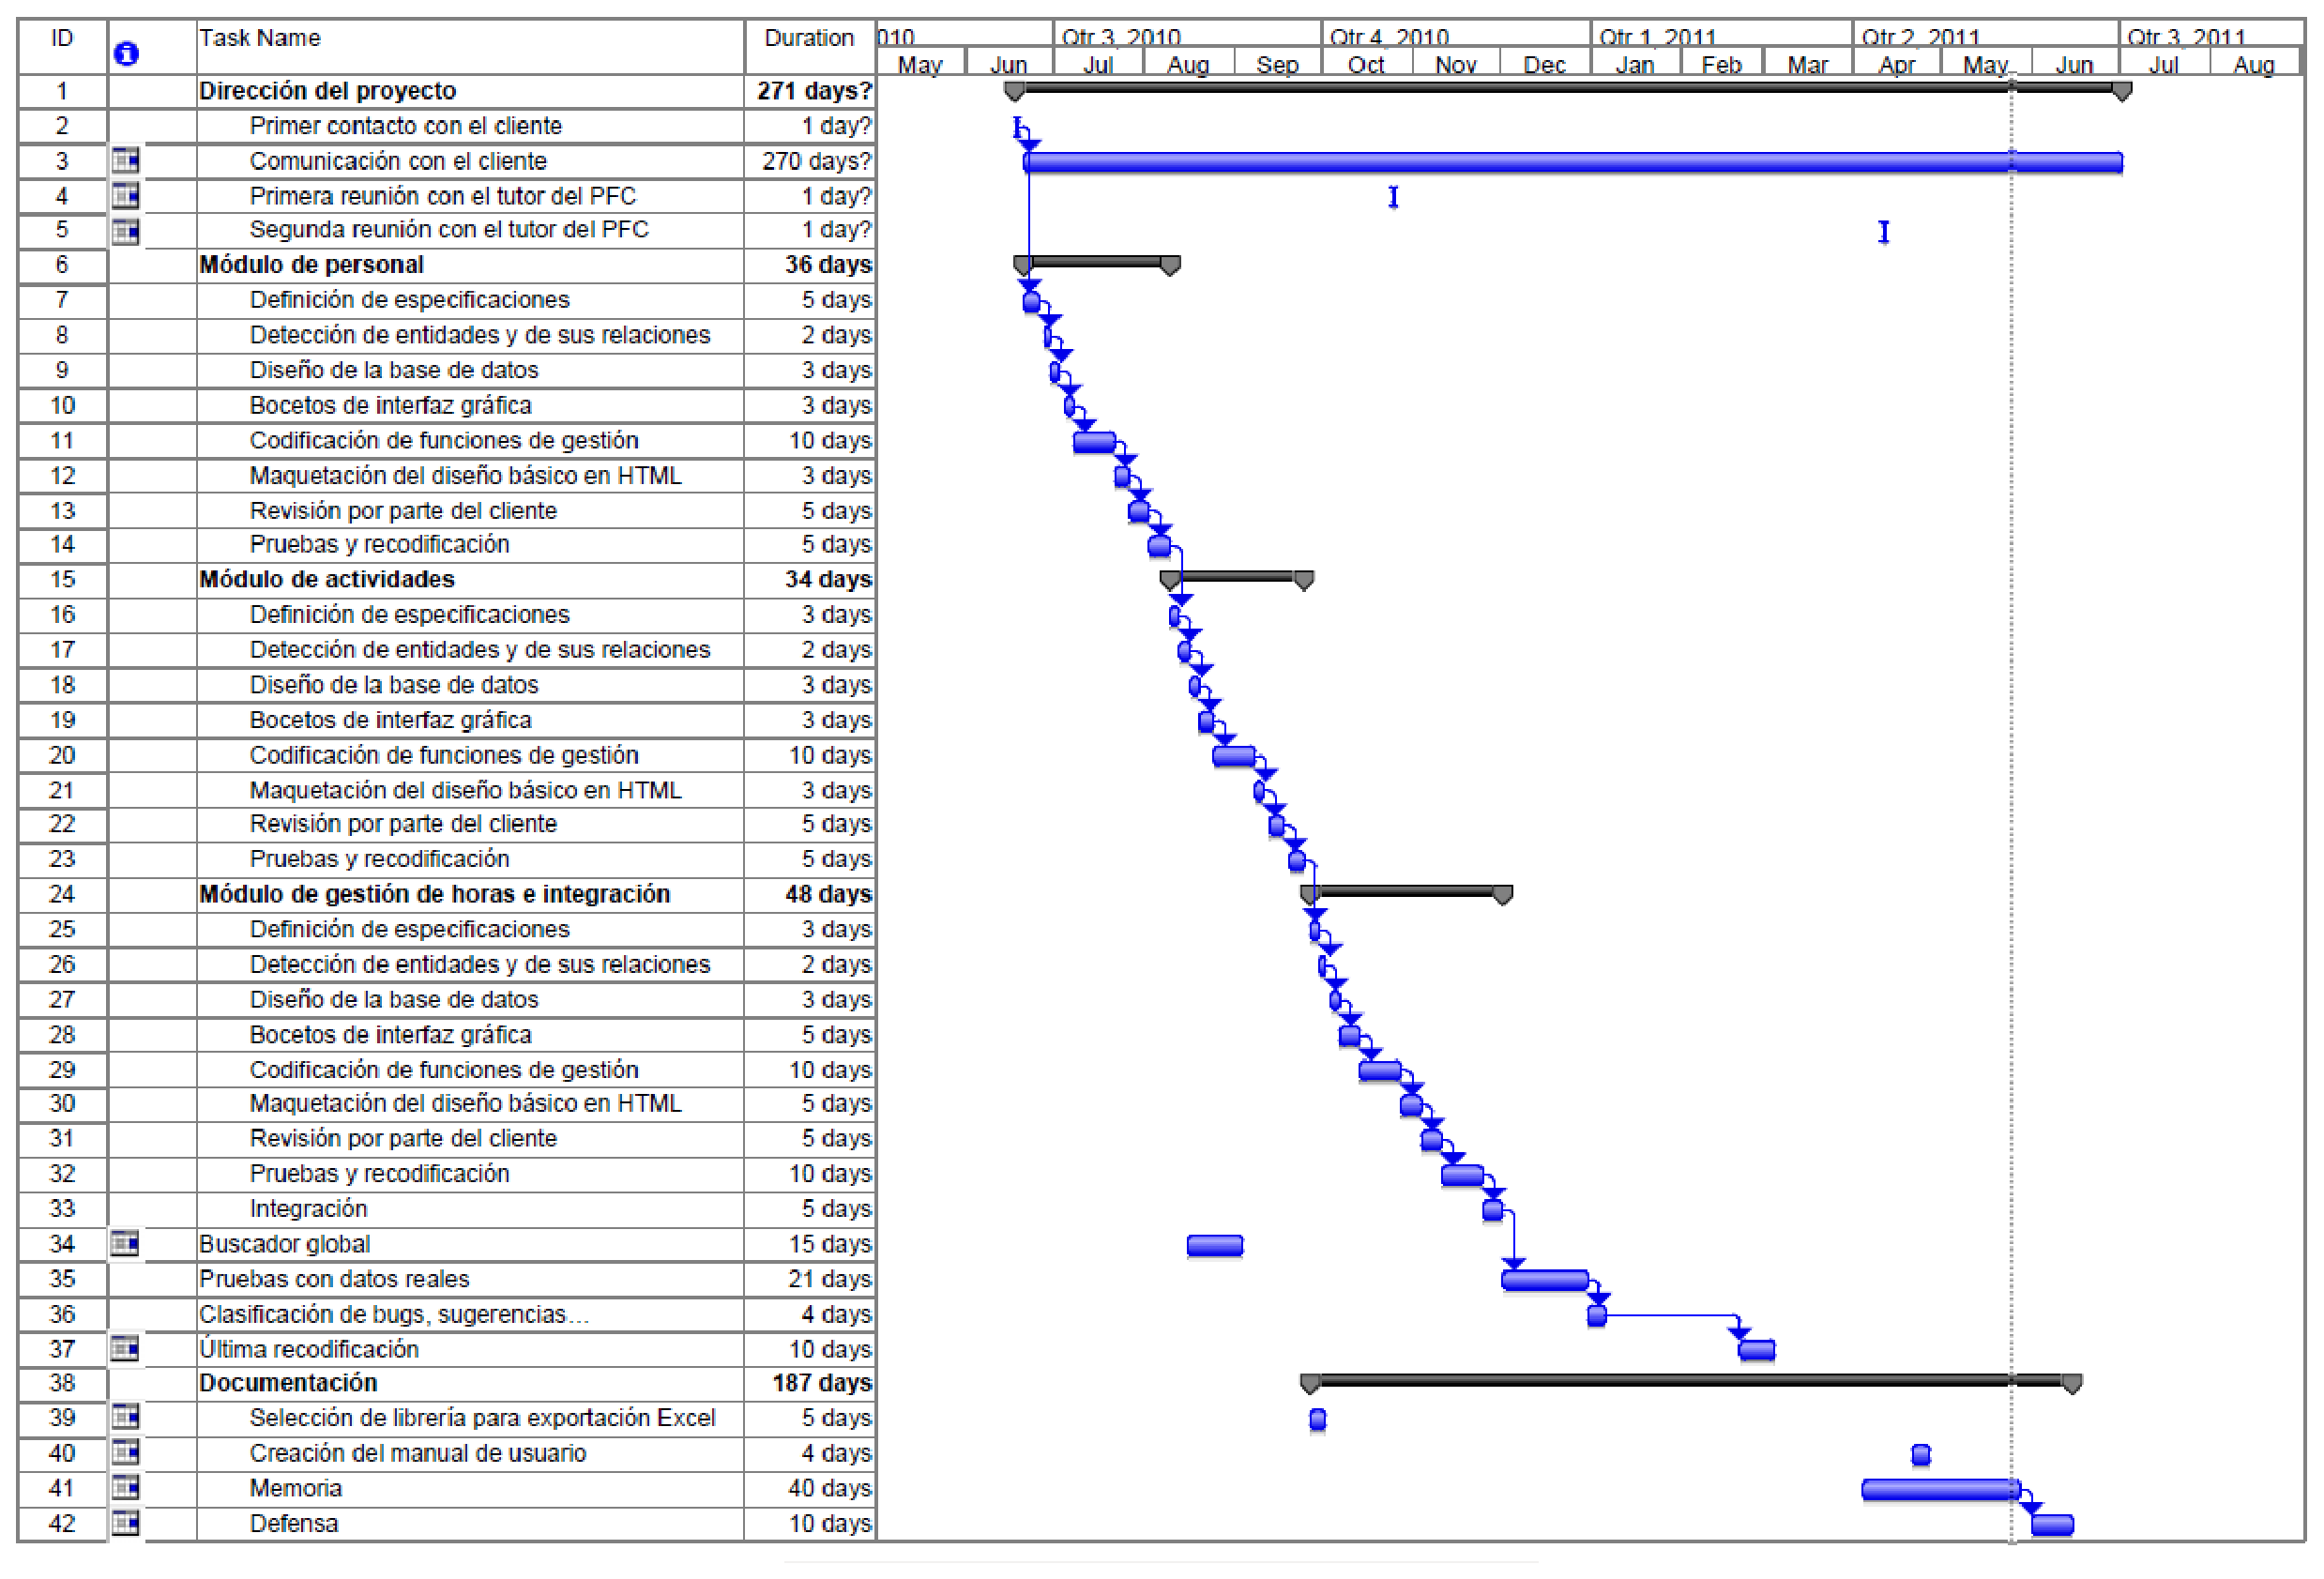
\epsfig{file=imagenes/gantt.eps,height=5in}
% 
% \end{minipage}
% } \quad\vfill \turnbox{90}{\usebox\myboxa}}
%%%%%%%%%%%%%%%%%%%%


 

\chapter{Análisis}
\label{chp:analisis}
\thispagestyle{empty}
\noindent \textit{En este capítulo se repasarán los requisitos y las
especificaciones tanto no funcionales como funcionales de cada parte de la
herramienta, y se definirán los casos de uso más representativos.}
\section{Especificación de los requisitos del sistema}

\subsection{Requisitos de interfaces de usuario}
\label{sec:requisitos_interfaz}

La interfaz de usuario está parcialmente definida por el sistema en el que se
integrará la nueva herramienta, pero dado el volumen de datos que va a
manejar, este va a ser un aspecto muy importante. Así, en esta sección se hará
un repaso al papel de las 5 'es' de la usabilidad definidas por Whitney
Quesenbery a partir de las propuestas de Jakob Nielsen:

\begin{description}
\item [Efectividad (Effective)] Si un usuario no puede completar la tarea que
quería realizar, lo demás no importa. En el caso del proyecto en cuestión, esta
va a ser la dimensión que va a tener un mayor peso.

\item [Eficiencia (Efficient)] Se refiere a la capacidad de la interfaz de
permitir realizar una tarea de forma correcta en el menor tiempo posible. Los
usuarios del sistema va a ser, en general, personal de administración, cuando no
ingenieros cualificados, por lo que esta es otra dimensión muy importante.

\item [Inspirador / Atractivo (Engaging)] Se refiere a cómo de satisfactorio
es el uso de la interfaz, a la calidad de la interacción. Esta es una de las
características fundamentales en proyectos abiertos al público, en el que se
pretende una participación masiva; sin embargo, el proyectante no considera que
deba tener mucho peso en este caso: la experiencia debe ser buena, pero no va a
ser un foco de atención.

\item [Tolerancia a errores (Error Tolerant)] Es muy importante que la interfaz
nos ayude en el proceso de consulta, adición y modificación de elementos, con el
objetivo de minimizar los errores en primer lugar, y de corregirlos una vez que
se han cometido.

\item [Fácil de aprender (Easy to Learn)] De nuevo, el hecho de que el sistema
vaya a ser usado por muy pocas personas, permite que no sea especialmente
importante invertir tiempo en diseñar una interfaz especialmente simple, lo
cual no es trivial cuando el sistema subyacente debe ser capaz de realizar
muchas tareas distintas.
\end{description}

\begin{figure}
\centering
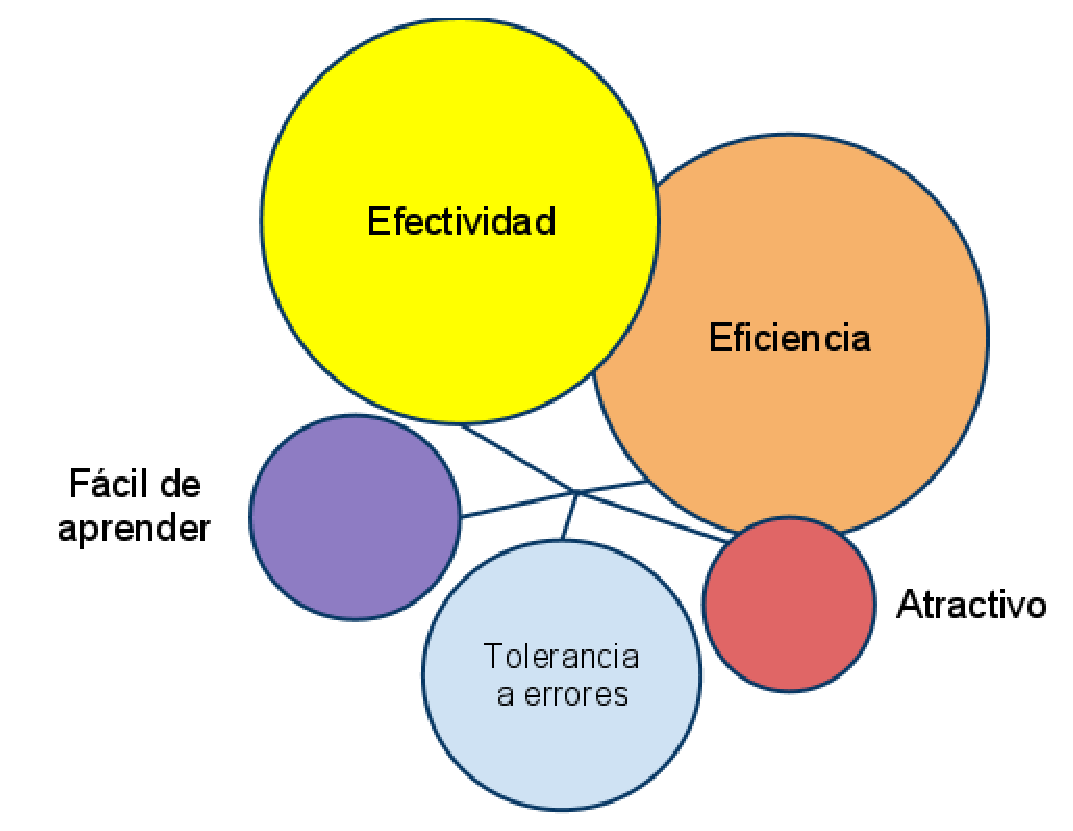
\epsfig{file=imagenes/usabilidad.eps,width=3.5in}
\caption{Importancia de las dimensiones de usabilidad.}
\label{fig:usabilidad}
\end{figure}

\subsection{Requisitos funcionales}
\label{sec:requisitos_funcionales}

En esta sección se listan los requisitos funcionales de la aplicación agrupados
por categorías:

\subsubsection{Requisitos funcionales de la gestión de personal}
\label{sec:requisitos_personal}

\begin{itemize}
\item El usuario puede buscar y visualizar los recursos humanos y sus
registros anuales presentes en el sistema, agrupados por cliente o
individualmente, donde se puedan consultar los siguientes datos:
  \begin{itemize}
  \item Año.
  \item Salario bruto.
  \item Seguridad Social a cargo de la empresa.
  \item Horas convenio.
  \item Horas asignadas / libres.
  \item Coste / hora.
  \item Notas
  \item Fecha y autoría de la última actualización
  \end{itemize}

\item Se podrá crear un nuevo empleado mediante el registro de
sus datos. Cada
empleado tiene un número indefinido de registros anuales, donde se almacenarán
datos como salario o número de horas del convenio. Para evitar confusiones, no
puede haber dos empleados con el mismo nombre y apellidos en el sistema: en
caso de que sea necesario, se añadirá algún tipo de marca manualmente
(ejemplos: bis, padre...). Cada empleado y cada registro anual se crea con un
identificador único. Será posible, a la hora de crear registros anuales,
renovar la información del empleado: con un solo clic, se creará un registro
anual nuevo inmediatamente posterior al más reciente con los mismos datos de
salario, etc.

\item Será posible modificar los datos de cada empleado y de sus registros
anuales. Por motivos de consistencia del sistema, no será posible cambiar el
cliente al que pertenece un empleado. En caso de que se haya asignado a un
cliente que no le corresponde por error, el empleado deberá ser borrado; si el
empleado cambia de una empresa cliente a otra, será necesario crear un nuevo
empleado. Sin embargo, el sistema no sabrá que son la misma persona: consultado
el cliente de la aplicación y tutor de empresa de este proyecto, no se ha
considerado imprescindible incluir tal característica por la poca probabilidad
de que suceda. Asimismo, tampoco podrá modificarse el año de un registro anual:
de resultar sus datos incorrectos para el año actual, deberán modificarse los
datos y añadirlos en el año que les correspondiera inicialmente; si el año ha
sido introducido por error, deberá borrarse.

\item Debe ser posible eliminar empleados y registros anuales. En caso de
eliminarse un empleado, todos sus registros anuales serán borrados en
cascada, y en caso de borrar un registro anual, las horas de asignadas a ese
año también serán borradas. Debe considerarse la poca o nula utilidad de borrar
un empleado que tiene horas asignadas en el sistema, esas horas se borrarían
igualmente: aunque un empleado no formase parte finalmente en la ejecución de un
proyecto y por tanto no deban justificarse su trabajo, es interesante para
realizar estudios estadísticos ver las horas que se presentaron para ese
empleado. La peligrosidad de borrar datos de este tipo por error ha llevado al
proyectante a decidir que esta acción solamente pueda ser llevada a cabo por el
usuario administrador del sistema (ver sección \ref{sec:usuarios_del_sistema}
para obtener más información acerca de los usuarios).
\end{itemize}

\subsubsection{Requisitos funcionales de la gestión de actividades}
\label{sec:gestion_actividades}

\begin{itemize}
\item El usuario puede buscar y visualizar las actividades registradas en
el sistema, agrupadas por cliente y proyectos, donde se puedan consultar los
siguientes datos:
  \begin{itemize}
  \item Nombre de la actividad.
  \item Descripción.
  \item Fecha de inicio.
  \item Fecha de fin.
  \item Horas presentadas.
  \item Horas aprobadas.
  \item Horas justificadas.
  \end{itemize}
 
\item Se podrán crear nuevas actividades empleado mediante el registro de
sus datos. Para evitar confusiones, y ya que, en general, no va a tener sentido,
no puede haber dos actividades con el mismo nombre en el sistema. Cada actividad
se crea con un identificador único.

\item Será posible modificar los datos de cada actividad. Por motivos de
consistencia del sistema, no será posible cambiar el proyecto al que pertenece
una actividad. En caso de que se haya asignado a un proyecto que no le
corresponde por error, la actividad deberá ser borrada.

\item Debe ser posible eliminar actividades, excepto en el caso de que el
proyecto esté concluido. En caso de
eliminarse una actividad, todos los datos de horas asociados a ella se borrarán
en cascada. Debe considerarse la poca o nula utilidad de borrar una actividad
que tiene horas asignadas en el sistema, esas horas se borrarían igualmente:
aunque una actividad no llegase a ejecutarse finalmente en el
desarrollo de un proyecto y por tanto no deban justificarse, es
interesante para realizar estudios estadísticos ver las horas que se presentaron
para ese actividad. La peligrosidad de borrar datos de este tipo por error ha
llevado al proyectante a decidir que esta acción solamente pueda ser llevada a
cabo por el usuario administrador del sistema (ver sección
\ref{sec:usuarios_del_sistema} para obtener más información acerca de los
usuarios).
\end{itemize}

\subsubsection{Requisitos funcionales de la consulta de datos e informes}
\label{sec:requisitos_informes}

\begin{itemize}
\item Debe ser posible visualizar cuántas horas tiene asignadas un recurso en
cada uno de sus registros anuales, así como el total de horas libres (sin
asignar hasta el total de su convenio). El concepto de total de horas asignadas
no es trivial y se define como la suma de los siguientes valores:
 
\begin{enumerate}
  \item En los proyectos en fase de presentación, las horas presentadas aunque
sean cero, siempre que no se hayan imputado horas aprobadas o justificadas. En
el último caso, se tomarán las de la fase más avanzada.
  \item En los proyectos en fase de aprobación, las horas aprobadas aunque sean
cero, siempre que no se hayan comenzado a imputar horas justificadas.
  \item En proyectos justificados o concluidos, las horas justificadas aunque
sean cero.
\end{enumerate}

Así, el número de horas libres se define como el total menos las asignadas,
calculadas como se acaba de describir.

\item Cualquier valor de horas visible en la vista del primer punto de esta
lista debe ser un enlace a un desglose mensual por actividades que muestre los
siguientes datos:
 \begin{itemize}
  \item Nombre del empleado.
  \item Año.
  \item Mes.
  \item Proyecto.
  \item Actividad.
  \item Horas presentadas.
  \item Horas aprobadas.
  \item Horas justificadas.
  \item Horas libres.
 \end{itemize}
Ese desglose debe tener además una serie de filtros por cliente, empleado, año,
mes, proyecto y actividad para adaptarse rápidamente a las necesidades del
usuario.

\item En la vista de los proyectos y sus actividades (sección
\ref{sec:gestion_actividades}) debe haber un resumen de horas agrupadas por año
para cada empleado en la tres fases de la gestión de proyectos: presentación,
aprobación y justificación.

\item También debe haber un informe de horas agrupadas por actividad para cada
empleado en la tres fases de la gestión de proyectos: presentación,
aprobación y justificación.

\item Adicionalmente, debe existir la posibilidad de descargar una hoja de
cálculo con la información de cada empleado acerca de su participación en el
proyecto para su etapa de presentación, aprobación y justificación. La hoja de
cálculo deberá tener tantas hojas como empleados participen en el proyecto.

\item Debe existir un informe resumen global de actividades y proyectos que sea
del mismo estilo a como se venían gestionando las horas hasta ahora. Así, debe
ser del mismo estilo que la figura \ref{fig:hoja_calculo} (pág.
\pageref{fig:hoja_calculo}) y también debe ser posible descargarla como hoja de
cálculo, de modo que se conserve totalmente la funcionalidad del viejo método.
Este informe debe tener las siguientes características:
 \begin{itemize}
  \item identificar cuándo un empleado no está dado de alta en la empresa.

  \item tener en cuenta el convenio de horas del recurso para informar acerca
  de las horas que le quedan libres en un año;

  \item cuando existe un conflicto, por ejemplo, se hayan imputado más horas
  de las que deberían, el valor aparece marcado en rojo;

  \item las columnas de proyectos siguen un código de colores para indicar el
  estado en que se encuentra el proyecto: sin comenzar y presentados, azul;
aprobados, verde; justificado o concluido, naranja; denegado, rojo.

  \item cada uno de los valores, incluidos los nombres de los recursos en
  cuestión, son un enlace a otra vista donde se darán detalles acerca
  del elemento.  En esta vista, también debe mostrarse el coste/hora de
  cada empleado para calcular el coste de la selección.
 \end{itemize}

\end{itemize}


\subsubsection{Requisitos funcionales de la gestión de horas}
\label{sec:requisitos_gestion_horas}

\begin{itemize}
 \item Debe ser posible asignar horas asociadas a la vez a personal y a
actividades. Dada la división de los proyectos subvencionados en fases de
presentación, aprobación y justificación, debe poderse asignar horas de cada
uno de esos tipos. Este hecho genera algunas restricciones:
 \begin{itemize}
  \item No se pueden asignar horas presentadas a proyectos en fase de
aprobación o superior.
  \item No se pueden asignar horas aprobadas a proyectos en fase de
justificación o terminados.
  \item No se pueden asignar horas justificadas a proyectos ya terminados.
 \end{itemize}
 \item Debe ser posible asignar horas a los empleados del cliente al que
pertenece la actividad a la que se están asignando horas, y a los empleados de
clientes que figuran como cooperantes en ese proyecto. La figura de cooperante
de proyecto es previa al inicio de este proyecto.
 \item A la hora de asignar horas a una actividad, debe ser posible ver
rápidamente qué empleados tienen ya horas imputadas.
 \item Cuando una actividad se extiende durante dos o más años distintos, debe
ser inmediato elegir, si procede, a que año pertenecen las horas. Esto es muy
útil, ya que es común realizar planificaciones de forma anual,
independientemente de la duración del proyecto.
 \item En caso de que la asignación no esté \textit{preplanificada} (aunque,
en general, lo estará), debe ser posible calcular el número de horas que se
puede trabajar en un periodo basándonos en el número de horas que se dedicarán
al día y teniendo en cuenta fines de semana y otros festivos.
 \item Ya que las asignaciones se realizan, en general, por lotes, es decir,
todas las de una actividad concreta de manera consecutiva, el sistema debe
facilitar una opción del tipo \textit{asignar y seguir}, que conservaría los
datos de actividad, tipo de horas... para que se reduzca el tiempo de gestión.
 \item Dado que muchas veces se aprueban exactamente las mismas horas que se
presentaron, o se justifican las mismas que se aprobaron, debe haber una
función capaz de trasladar idénticamente las horas de un estado a otro. El
ahorro de tiempo de gestión que se produciría en estos casos es irrenunciable,
y puede llegar a ser útil incluso cuando, sin ser idénticas, las horas de un
tipo son similares a las del tipo anterior: en ese caso, solo habría que
modificar las pequeñas variaciones.
 \item La asignación de horas a un periodo se repartirá internamente por
meses (no días), de manera que las horas asignadas a un periodo que comprenda
dos meses o más se repartirán porcentualmente teniendo en cuenta el número de
días laborables de cada mes, y cuando sea posible, en múltiplos de 5. Debido a
la excesiva complejidad que se añadiría, no se tienen en cuenta las horas del
empleado en otros proyectos en el momento de la asignación.
 \item El sistema debe detectar las inconsistencias derivadas de un exceso de
horas asignadas a un empleado en un mes dado o al global del año de acuerdo a
su convenio.
 \item Debe ser posible modificar una asignación, atendiendo a las mismas
restricciones del primer punto de esta lista.
 \item Para simplificar, el concepto de borrar horas se satisface con el de
modificar asignando cero horas. De esta manera, el \textit{borrado} de horas
sigue las mismas restricciones que cualquier otra modificación.
 \item La detección de inconsistencias no debe requerir de ninguna acción del
usuario. Cualquier inconsistencia será marcada en rojo automáticamente, a la
espera de las acciones correctoras de los técnicos. Al asignar horas, el
sistema debe advertir instantáneamente de las inconsistencias producidas por
esa asignación.
\end{itemize}

\subsubsection{Requisitos funcionales de la búsqueda}

Hemos visto que el primer requisito de la gestión de recursos y de actividades
es la capacidad de buscar y visualizar la información. Para ello, cada parte
dispone de su propio filtro con funcionalidades avanzadas, por ejemplo: al
buscar personal, lo podremos hacer por nombre, cliente, año de inicio, coste
hora, ubicación o una combinación de todos; al buscar actividades, lo podremos
hacer mediante su nombre, proyecto, cliente o una combinación de todos.

Además, de acuerdo con el cliente pero a propuesta del proyectante, se
determinó que sería muy útil implementar un buscador global, característica de
la que la aplicación carecía, de manera que se pudieran encontrar clientes,
proyectos y recursos y desde allí tener acceso
a cada parte del sistema relacionada, entre ellas, los nuevos módulos de
personal y actividades.

Para dar más sentido a este buscador, este debe ser simple, accesible desde el
inicio de la sesión y a lo largo de toda ella, instantáneo, versátil,
y debe priorizar datos y dar acceso a todas las funcionalidades. Para
explicar como se logrará todo lo anterior, se presenta a continuación cada
funcionalidad brevemente detallada:

\begin{description}
\item [Simple] El buscador consistirá en una única caja de búsqueda que
devolverá los resultados (clientes, proyectos y recursos humanos) coincidentes
con la consulta del usuario. Para búsqueda avanzada, deberán emplearse los
filtros específicos de cada módulo.

\item [Accesible] El buscador se convertirá en la página de inicio de la
aplicación, y estará disponible a lo largo de toda la sesión en la barra de
menú superior.

\item [Instantáneo] Gracias al uso de AJAX, el buscador será instantáneo, de
manera que cada vez que el usuario haga clic en una letra, el resultado se
actualizará automáticamente. En combinación con la siguiente característica,
los resultados deberían ser los esperados cuando solamente se hayan tecleado
unas pocas letras del elemento buscado.

\item [Priorizar datos] En lugar de ordenar los resultados por el número de
concurrencias o por identificador, el buscador ordenará los recursos humanos
por orden alfabético. En el caso de los clientes y de los proyectos, se irá un
paso más allá para tener en cuenta el número de proyectos que tiene un cliente
y el número de expedientes que tiene un proyecto. Así, los clientes con más
proyectos y los proyectos con más expedientes se mostrarán antes. Por último,
cuando una consulta devuelva los tres tipos de datos, el orden será clientes,
recursos, proyectos.

\item [Versátil] El buscador tendrá en cuenta las características más
importantes de cada elemento. Así, no solamente buscará clientes por su nombre,
sino también por su acrónimo, teléfono, dirección, descripción... Algo similar
ocurrirá con los proyectos y los recursos, de manera que si buscamos el nombre
de un cliente, se mostrará en primer lugar ese cliente, gracias a la prioridad
de datos global descrita en el apartado anterior, y también se mostrarán sus
recursos humanos y proyectos. Se implementarán, asimismo, funciones de
paginación y la posibilidad de mostrar únicamente clientes, proyectos o
recursos.

Otra característica que se implementará de cara a la versatilidad del
buscador es la capacidad para devolver resultados incluso cuando el usuario
cometa algún error. Aunque se realizará simplemente truncando la consulta cuando
no se encuentren resultados, se espera que sea suficientemente útil.

\item [Dar acceso] La idea de esta parte es la de imitar los accesos directos
que ofrecen las principales buscadores (ver figura \ref{fig:enlaces_buscador}).
Desde un cliente, podrá accederse a proyectos, facturas, contratos, archivos y
por supuesto, personal y actividades. Desde un proyecto, podrá accederse a sus
expedientes, a sus facturas y a sus actividades.

\end{description}

\begin{figure}
\centering

\epsfig{file=imagenes/enlaces_buscador.eps,width=5.28in}
\caption{Enlaces de interés desde el buscador de Google.}
\label{fig:enlaces_buscador}
\end{figure}


\section{Requisitos lógicos de la base de datos}

La base de datos es uno de los componentes fundamentales de la aplicación. Se
va a hacer uso de una base de datos existente llamada \textit{ingenieria}, en la
que se integrarán las tablas necesarias para guardar todas la información
necesaria para cumplir los requisitos especificados en la sección
\ref{sec:requisitos_funcionales}. Las tablas que se añadirán son las siguientes:

\begin{description}
\item [actividad] Almacenará los datos de las actividades de cada
proyecto.

\item [coste\_personal] Contendrá la información de cada registro anual
de los empleados.

\item [personal] Guardará la información acerca de cada empleado.

\item [personal\_actividad] Guarda información básica acerca de cada asignación
realizada.

\item [personal\_horas] Almacenará los datos de horas mensuales para cada
empleado en cada actividad.
\end{description}

Los detalles sobre el diseño de la base de datos pueden consultarse en el
capítulo \ref{chp:diseno}.

\section{Casos de uso}
\label{sec:casos_de_uso}

En esta sección se especificarán los casos de uso más relevantes para cada
parte del sistema. Aunque la división física de los sistemas no es evidente, a
la hora de organizar los casos de uso se ha elegido una división lógica con
tres sistemas básicos: gestor de personal, gestor de actividades, y gestor de
horas e informes. El buscador global es tan simple que no se ha considerado
necesario elaborar un caso de uso específico.

\subsection{Gestor de personal}

\begin{figure}
\centering
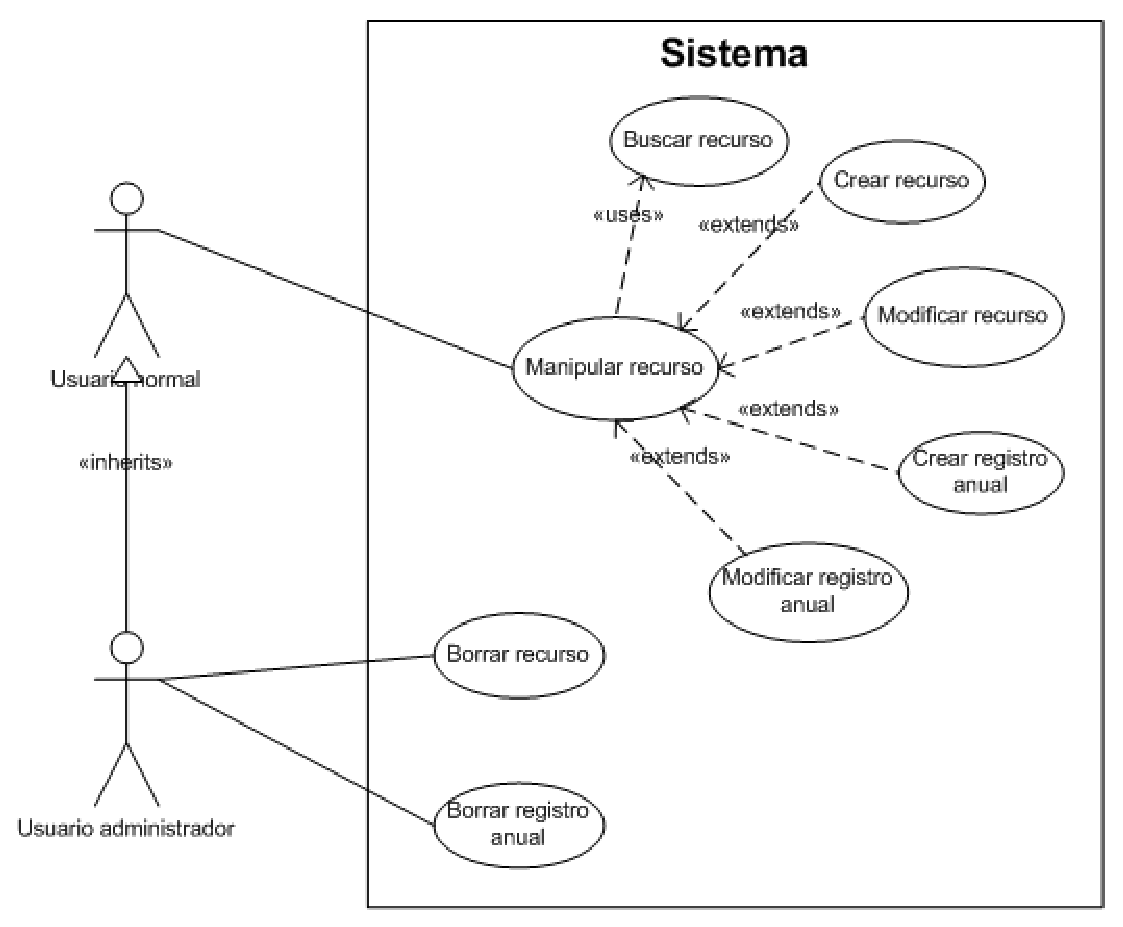
\epsfig{file=imagenes/CU_recursos.eps,width=5.28in}
\caption{Diagrama de casos de uso para los recursos.}
\label{fig:CU_recursos}
\end{figure}

Las especificaciones que hacen referencia al gestor de personal están
descritas en la sección \ref{sec:requisitos_personal}. Todos los casos de uso
relacionados con la gestión de personal que se detallarán en este capítulo, así
como las relaciones entre los mismos, están representados en el diagrama de la
figura \ref{fig:CU_recursos}. Los usuarios del sistema y sus funciones generales
están descritos en profundidad en la sección \ref{sec:usuarios_del_sistema}.

\begin{tabular}{|p{1.25in}|p{3.65in}|}\hline
\textbf{Caso de uso} & \textbf{Buscar recurso}\\\hline\hline
\textbf{Descripción} & Búsqueda de un recurso atendiendo a diversos
parámetros\\\hline
\textbf{Actores} & Usuario normal \newline Usuario administrador\\\hline
\textbf{Precondiciones} & El usuario está autenticado en el sistema y
tiene permisos para ver el módulo de recursos\\\hline
\textbf{Pasos} & 
  \begin{enumerate}
   \item El usuario introduce los datos en los campos de búsqueda.
   \item El usuario comprueba si la búsqueda es satisfactoria, y si no lo es,
vuelve al primer paso.
  \end{enumerate}
\\\hline
\textbf{Variaciones} & \\\hline
\textbf{Cuestiones} & \\\hline
\end{tabular}

\begin{tabular}{|p{1.25in}|p{3.65in}|}\hline
\textbf{Caso de uso} & \textbf{Crear recurso}\\\hline\hline
\textbf{Descripción} & Crear un nuevo recurso en el sistema. Los
atributos propios de un recurso están descritos en la sección
\ref{sec:requisitos_personal}\\\hline
\textbf{Actores} & Usuario normal \newline Usuario administrador\\\hline
\textbf{Precondiciones} & El usuario está autenticado en el sistema y
tiene permisos para ver el módulo de recursos\\\hline
\textbf{Pasos} & 
  \begin{enumerate}
   \item El usuario introduce los atributos del nuevo recurso.
   \item El usuario comprueba que el recurso se ha añadido correctamente; si
no, el sistema dará un mensaje de error y el usuario debería volver al primer
paso e introducir los datos correctamente.
  \end{enumerate}
\\\hline
\textbf{Variaciones} & En cualquier momento, el usuario puede cancelar
la operación.\\\hline
\textbf{Cuestiones} & Hay una serie de campos obligatorios (nombre,
cliente...) y según los requisitos, no puede haber dos recursos
con el mismo nombre en la misma empresa.\\\hline
\end{tabular}

\begin{tabular}{|p{1.25in}|p{3.65in}|}\hline
\textbf{Caso de uso} & \textbf{Modificar recurso}\\\hline\hline
\textbf{Descripción} & Modificar los datos de un recurso en el sistema. Los
atributos propios de un recurso están descritos en la sección
\ref{sec:requisitos_personal}\\\hline
\textbf{Actores} & Usuario normal \newline Usuario administrador\\\hline
\textbf{Precondiciones} & El usuario está autenticado en el sistema y
tiene permisos para ver el módulo de recursos\newline El usuario ha
buscado el recurso usando el caso de uso «Buscar recurso»\\\hline
\textbf{Pasos} & 
  \begin{enumerate}
   \item El usuario introduce los atributos actualizados del recurso.
   \item El usuario comprueba que el recurso se ha modificado correctamente; si
no, el sistema dará un mensaje de error y el usuario debería volver al primer
paso e introducir los datos correctamente.
  \end{enumerate}
\\\hline
\textbf{Variaciones} & En cualquier momento, el usuario puede cancelar
la operación.\\\hline
\textbf{Cuestiones} & Hay una serie de campos obligatorios (nombre,
cliente...) y según los requisitos, no puede haber dos recursos
con el mismo nombre en la misma empresa.\\\hline
\end{tabular}

\begin{tabular}{|p{1.25in}|p{3.65in}|}\hline
\textbf{Caso de uso} & \textbf{Crear registro anual}\\\hline\hline
\textbf{Descripción} & Crear un nuevo registro anual para un recurso del
sistema. Los atributos propios de un recurso están descritos en la sección
\ref{sec:requisitos_personal}\\\hline
\textbf{Actores} & Usuario normal \newline Usuario administrador\\\hline
\textbf{Precondiciones} & El usuario está autenticado en el sistema y
tiene permisos para ver el módulo de recursos \newline El usuario ha
buscado un recurso existente usando el caso de uso «Buscar recurso».\\\hline
\textbf{Pasos} & 
  \begin{enumerate}
   \item El usuario introduce los atributos del nuevo registro anual.
   \item El usuario comprueba que el registro se ha añadido correctamente; si
no, el sistema dará un mensaje de error y el usuario debería volver al primer
paso e introducir los datos correctamente.
  \end{enumerate}
\\\hline
\textbf{Variaciones} & En cualquier momento, el usuario puede cancelar
la operación.\\\hline
\textbf{Cuestiones} & Hay una serie de campos obligatorios (año,
coste/hora...) y según los requisitos, no puede haber dos registros
anuales que hagan referencia a un mismo año.\\\hline
\end{tabular}

\begin{tabular}{|p{1.25in}|p{3.65in}|}\hline
\textbf{Caso de uso} & \textbf{Modificar registro anual}\\\hline\hline
\textbf{Descripción} & Modificar los datos de un registro anual de un recurso
del sistema. Los atributos propios de un recurso están descritos en la sección
\ref{sec:requisitos_personal}\\\hline
\textbf{Actores} & Usuario normal \newline Usuario administrador\\\hline
\textbf{Precondiciones} & El usuario está autenticado en el sistema y
tiene permisos para ver el módulo de recursos\newline El usuario ha
buscado el recurso que tiene registros anuales usando el caso de uso «Buscar
recurso»\\\hline
\textbf{Pasos} & 
  \begin{enumerate}
   \item El usuario introduce los atributos actualizados del registro anual.
   \item El usuario comprueba que el recurso se ha modificado correctamente; si
no, el sistema dará un mensaje de error y el usuario debería volver al primer
paso e introducir los datos correctamente.
  \end{enumerate}
\\\hline
\textbf{Variaciones} & En cualquier momento, el usuario puede cancelar
la operación.\\\hline
\textbf{Cuestiones} & Hay una serie de campos obligatorios (año,
coste/hora...) y según los requisitos, no puede haber dos registros
anuales que hagan referencia a un mismo año.\\\hline
\end{tabular}

\begin{tabular}{|p{1.25in}|p{3.65in}|}\hline
\textbf{Caso de uso} & \textbf{Borrar recurso}\\\hline\hline
\textbf{Descripción} & Borrar los datos de un recurso en el sistema, junto con
sus registros anuales. \\\hline
\textbf{Actores} & Usuario administrador\\\hline
\textbf{Precondiciones} & El administrador ha
buscado el recurso usando el caso de uso «Buscar recurso»\\\hline
\textbf{Pasos} & 
  \begin{enumerate}
   \item El administrador elige la opción de borrar recurso.
   \item El administrador confirma que desea borrar el recurso seleccionado.
   \item El administrador comprueba que el recurso se ha borrado
correctamente; si no, el sistema dará un mensaje de error.
  \end{enumerate}
\\\hline
\textbf{Variaciones} & El administrador puede cancelar la operación en lugar
de confirmarla.\\\hline
\textbf{Cuestiones} & Al borrar un recurso, se borran todas sus horas asignadas
y sus registros anuales.\\\hline
\end{tabular}

\begin{tabular}{|p{1.25in}|p{3.65in}|}\hline
\textbf{Caso de uso} & \textbf{Borrar registro anual}\\\hline\hline
\textbf{Descripción} & Borrar un registro anual de un recurso
del sistema.
\ref{sec:requisitos_personal}\\\hline
\textbf{Actores} & Usuario administrador\\\hline
\textbf{Precondiciones} & El administrador ha buscado el recurso que tiene
registros anuales usando el caso de uso «Buscar recurso»\\\hline
\textbf{Pasos} & 
  \begin{enumerate}
   \item El administrador elige la opción de borrar registro anual.
   \item El administrador confirma que desea borrar el registro anual.
   \item El administrador comprueba que el registro anual se ha borrado
correctamente; sino, el sistema dará un mensaje de error.
  \end{enumerate}
\\\hline
\textbf{Variaciones} & El administrador puede cancelar la operación en lugar
de confirmarla.\\\hline
\textbf{Cuestiones} & Al borrar un registro anual, se borrarán todas las
horas asignadas a ese año.\\\hline
\end{tabular}


\subsection{Gestor de actividades}

\begin{figure}
\centering
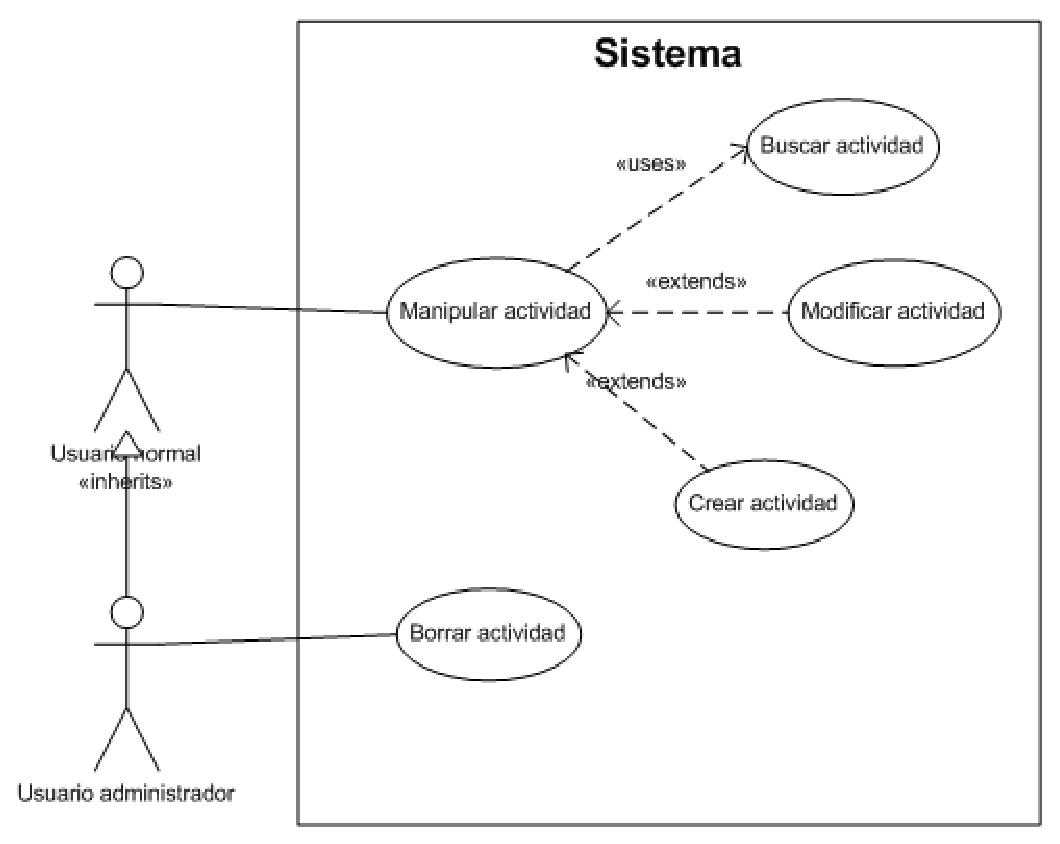
\epsfig{file=imagenes/CU_actividades.eps,width=5in}
\caption{Diagrama de casos de uso para las actividades.}
\label{fig:CU_actividades}
\end{figure}

Las especificaciones que hacen referencia al gestor de actividades están
descritas en la sección \ref{sec:gestion_actividades}. Todos los casos de uso
relacionados con la gestión de actividades que se detallarán en este capítulo,
así como las relaciones entre los mismos, están representados en el diagrama de
la figura \ref{fig:CU_actividades}. Los usuarios del sistema y sus funciones
generales están descritos en profundidad en la sección
\ref{sec:usuarios_del_sistema}.

\begin{tabular}{|p{1.25in}|p{3.65in}|}\hline
\textbf{Caso de uso} & \textbf{Buscar actividad}\\\hline\hline
\textbf{Descripción} & Búsqueda de una actividad atendiendo a diversos
parámetros\\\hline
\textbf{Actores} & Usuario normal \newline Usuario administrador\\\hline
\textbf{Precondiciones} & El usuario está autenticado en el sistema y
tiene permisos para ver el módulo de actividades. \\\hline
\textbf{Pasos} & 
  \begin{enumerate}
   \item El usuario introduce los datos en los campos de búsqueda.
   \item El usuario comprueba si la búsqueda es satisfactoria, y si no lo es,
vuelve al primer paso.
  \end{enumerate}
\\\hline
\textbf{Variaciones} & \\\hline
\textbf{Cuestiones} & \\\hline
\end{tabular}

\begin{tabular}{|p{1.25in}|p{3.65in}|}\hline
\textbf{Caso de uso} & \textbf{Crear actividad}\\\hline\hline
\textbf{Descripción} & Crear una nueva actividad en el sistema. Los
atributos propios de una actividad están descritos en la sección
\ref{sec:gestion_actividades}\\\hline
\textbf{Actores} & Usuario normal \newline Usuario administrador\\\hline
\textbf{Precondiciones} & El usuario está autenticado en el sistema y
tiene permisos para ver el módulo de actividades. El proyecto al que desea
añadir la actividad no está concluido. \\\hline
\textbf{Pasos} & 
  \begin{enumerate}
   \item El usuario introduce los atributos de la nueva actividad.
   \item El usuario comprueba que la actividad se ha añadido correctamente; si
no, el sistema dará un mensaje de error y el usuario debería volver al primer
paso e introducir los datos correctamente.
  \end{enumerate}
\\\hline
\textbf{Variaciones} & En cualquier momento, el usuario puede cancelar
la operación.\\\hline
\textbf{Cuestiones} & Hay una serie de campos obligatorios (nombre,
proyecto, fechas...) y según los requisitos, no puede haber dos actividades
con el mismo nombre en un mismo proyecto.\\\hline
\end{tabular}

\begin{tabular}{|p{1.25in}|p{3.65in}|}\hline
\textbf{Caso de uso} & \textbf{Modificar actividad}\\\hline\hline
\textbf{Descripción} & Modificar los datos de una actividad en el sistema. Los
atributos propios de una actividad están descritos en la sección
\ref{sec:gestion_actividades}. \\\hline
\textbf{Actores} & Usuario normal \newline Usuario administrador\\\hline
\textbf{Precondiciones} & El usuario está autenticado en el sistema y
tiene permisos para ver el módulo de actividades. \newline El usuario ha
buscado la actividad usando el caso de uso «Buscar recurso». \newline La
actividad pertenece a un proyecto que no está concluido.\\\hline
\textbf{Pasos} & 
  \begin{enumerate}
   \item El usuario introduce los atributos actualizados de la actividad.
   \item El usuario comprueba que la actividad se ha modificado correctamente;
si no, el sistema dará un mensaje de error y el usuario debería volver al primer
paso e introducir los datos correctamente.
  \end{enumerate}
\\\hline
\textbf{Variaciones} & En cualquier momento, el usuario puede cancelar
la operación.\\\hline
\textbf{Cuestiones} & Hay una serie de campos obligatorios (nombre,
proyecto, fechas...) y según los requisitos, no puede haber dos actividades
con el mismo nombre en el mismo proyecto.\\\hline
\end{tabular}

\begin{tabular}{|p{1.25in}|p{3.65in}|}\hline
\textbf{Caso de uso} & \textbf{Borrar actividad}\\\hline\hline
\textbf{Descripción} & Borrar los datos de una actividad en el sistema. \\\hline
\textbf{Actores} & Usuario administrador\\\hline
\textbf{Precondiciones} & El administrador ha
buscado la actividad usando el caso de uso «Buscar actividad».\\\hline
\textbf{Pasos} & 
  \begin{enumerate}
   \item El administrador elige la opción de borrar actividad.
   \item El administrador confirma que desea borrar la actividad seleccionada.
   \item El administrador comprueba que la actividad se ha borrado
correctamente; si no, el sistema dará un mensaje de error.
  \end{enumerate}
\\\hline
\textbf{Variaciones} & El administrador puede cancelar la operación en lugar
de confirmarla.\\\hline
\textbf{Cuestiones} & Al borrar una actividad, se borran todas sus horas
asignadas a cualquier recurso.\\\hline
\end{tabular}

\subsection{Gestor de horas e informes}

\begin{figure}
\centering
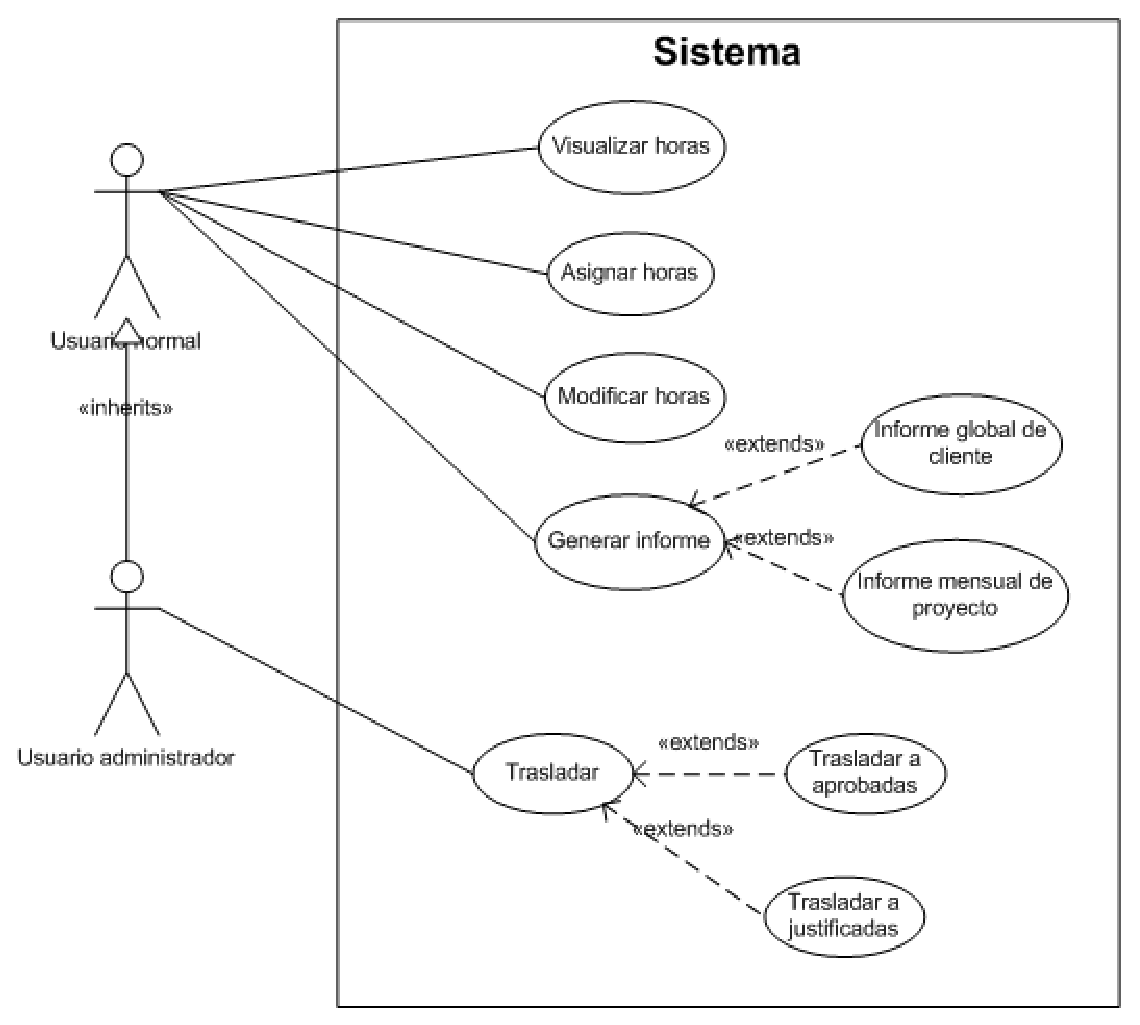
\epsfig{file=imagenes/CU_horas.eps,width=5.28in}
\caption{Diagrama de casos de uso para las gestión de horas.}
\label{fig:CU_horas}
\end{figure}

Las especificaciones que hacen referencia a la gestión de horas están
descritas en la sección \ref{sec:requisitos_gestion_horas}. Todos los casos de
uso relacionados con la gestión de horas que se detallarán en este
capítulo, así como las relaciones entre los mismos, están representados en el
diagrama de la figura \ref{fig:CU_horas}. Los usuarios del sistema y sus
funciones generales están descritos en profundidad en la sección
\ref{sec:usuarios_del_sistema}.

\begin{tabular}{|p{1.25in}|p{3.65in}|}\hline
\textbf{Caso de uso} & \textbf{Visualizar detalle de horas}\\\hline\hline
\textbf{Descripción} & Visualizar las horas asociadas a actividades o recursos,
según una serie de parámetros. \\\hline
\textbf{Actores} & Usuario normal \newline Usuario administrador\\\hline
\textbf{Precondiciones} & El usuario está autenticado en el sistema y
tiene permisos para ver los módulos de actividades o recursos.\\\hline
\textbf{Pasos} & 
  \begin{enumerate}
   \item El usuario pincha sobre el valor de horas que desea visualizar en
cualquier sitio dentro de los módulos de recursos o actividades.
  \end{enumerate}
\\\hline
\textbf{Variaciones} & Si el usuario no quiere ver el detalle de horas,
basta con buscar los recursos o las actividades para obtener información
básica usando los casos de uso «Buscar recurso» y «Buscar actividad».\\\hline
\textbf{Cuestiones} & Este caso de uso dirige al usuario a una nueva
ventana de su navegador.\\\hline
\end{tabular}

\begin{tabular}{|p{1.25in}|p{3.65in}|}\hline
\textbf{Caso de uso} & \textbf{Asignar horas}\\\hline\hline
\textbf{Descripción} & Asignar un número determinado de horas a un recurso en
una actividad. \\\hline
\textbf{Actores} & Usuario normal | Usuario administrador\\\hline
\textbf{Precondiciones} & El usuario está autenticado en el sistema y
tiene permisos para ver los módulos de actividades o recursos. El
recurso tiene registros anuales para el periodo que dura la actividad,
que debe pertenecer a un proyecto no concluido.\\\hline
\textbf{Pasos} & 
  \begin{enumerate}
   \item El usuario selecciona la opción asignar horas en la actividad deseada.
   \item El usuario elige el recurso al que se van a asignar las horas, el
tipo de horas (con restricciones según el estado del proyecto) y el rango de
fechas en el que se distribuirán las horas.
   \item El usuario confirma que las horas se han asignado correctamente; si
no, el sistema dará un mensaje de error y el usuario deberá volver al primer
punto de esta lista.
  \end{enumerate}
\\\hline
\textbf{Variaciones} & El usuario puede cancelar la operación en
cualquier momento. Si se genera alguna inconsistencia, el sistema advierte al
usuario y enlaza al detalle de horas de la asignación.\\\hline
\textbf{Cuestiones} & La asignación se realiza, cuando es posible, por
bloques de 5 horas. Una asignación puede sobrescribir otra asignación
anterior. \\\hline
\end{tabular}

\begin{tabular}{|p{1.25in}|p{3.65in}|}\hline
\textbf{Caso de uso} & \textbf{Modificar horas}\\\hline\hline
\textbf{Descripción} & Modificar una asignación de horas a nivel de mes.
\\\hline
\textbf{Actores} & Usuario normal \newline Usuario administrador\\\hline
\textbf{Precondiciones} & El usuario está autenticado en el sistema y
tiene permisos para ver los módulos de actividades o recursos. Las horas
asignadas son modificables según las restricciones por el estado del
proyecto. \\\hline
\textbf{Pasos} & 
  \begin{enumerate}
   \item El usuario pincha sobre las horas que desea modificar en el detalle
mensual de horas.
   \item El usuario introduce el nuevo valor y confirma la operación.
  \end{enumerate}
\\\hline
\textbf{Variaciones} & El usuario puede cancelar la operación en
cualquier momento.\\\hline
\textbf{Cuestiones} & Una modificación de este tipo modifica la suma
global de horas asignadas, es decir, la diferencia con las horas previas
no se sustrae o se añade en otro mes.\\\hline
\end{tabular}

\begin{tabular}{|p{1.25in}|p{3.65in}|}\hline
\textbf{Caso de uso} & \textbf{Generar informe global de cliente}\\\hline\hline
\textbf{Descripción} & Genera una hoja de cálculo con el estado actual de la
base de datos resumiendo la asignación de horas para todos los empleados del
cliente en todos los proyectos.
\\\hline
\textbf{Actores} & Usuario normal \newline Usuario administrador\\\hline
\textbf{Precondiciones} & El usuario está autenticado en el sistema y
tiene permisos para ver los módulos de actividades o recursos. \\\hline
\textbf{Pasos} & 
  \begin{enumerate}
   \item El usuario pincha sobre el enlace de generación de la hoja de cálculo.
   \item El usuario abre o guarda el archivo (el comportamiento varía según el
navegador empleado).
  \end{enumerate}
\\\hline
\textbf{Variaciones} & \\\hline
\textbf{Cuestiones} & La generación puede llevar varios segundos
dependiendo de la cantidad de datos a exportar.\\\hline
\end{tabular}

\begin{tabular}{|p{1.25in}|p{3.65in}|}\hline
\textbf{Caso de uso} & \textbf{Generar informe mensual de
proyecto}\\\hline\hline
\textbf{Descripción} & Genera una hoja de cálculo con el estado actual de la
base de datos resumiendo la asignación de horas por mes para todos los empleados
del cliente en todos los proyectos. Cada empleado tiene su propia hoja en el
archivo.
\\\hline
\textbf{Actores} & Usuario normal \newline Usuario administrador\\\hline
\textbf{Precondiciones} & El usuario está autenticado en el sistema y
tiene permisos para ver los módulos de actividades o recursos. \\\hline
\textbf{Pasos} & 
  \begin{enumerate}
   \item El usuario pincha sobre el enlace de generación de la hoja de cálculo
adecuado: presentación, aprobación o justificación.
   \item El usuario abre o guarda el archivo (el comportamiento varía según el
navegador empleado).
  \end{enumerate}
\\\hline
\textbf{Variaciones} & \\\hline
\textbf{Cuestiones} & La generación puede llevar varios segundos
dependiendo de la cantidad de datos a exportar.\\\hline
\end{tabular}

\begin{tabular}{|p{1.25in}|p{3.65in}|}\hline
\textbf{Caso de uso} & \textbf{Trasladar horas}\\\hline\hline
\textbf{Descripción} & Traslada todas las horas presentadas a aprobadas, o
todas las aprobadas a justificadas, para un proyecto concreto, y lo hace
actividad por actividad y empleado por empleado.
\\\hline
\textbf{Actores} & Usuario administrador\\\hline
\textbf{Precondiciones} & El administrador ha
buscado la actividad usando el caso de uso «Buscar actividad». \\\hline
\textbf{Pasos} & 
  \begin{enumerate}
   \item El administrador pincha sobre el enlace de traslación de horas
adecuado.
   \item El administrador confirma la operación y comprueba que las horas se han
trasladado correctamente.
  \end{enumerate}
\\\hline
\textbf{Variaciones} & El administrador puede cancelar la operación en
lugar de confirmarla. \\\hline
\textbf{Cuestiones} & La traslación conserva todas las horas, incluso
si generan inconsistencias.\\\hline
\end{tabular}

\newpage
\section{Protección de datos}

Ingeniería e Innovación necesita poseer datos sensibles de sus clientes y
de los empleados de estos para llevar a cabo su actividad. Por ello, en los
contratos que firma con sus clientes, se siguen escrupulosamente las pautas
marcadas por la Ley Orgánica 15/1999 de 13 de diciembre de Protección de Datos
de Carácter Personal (LOPD). Así, los clientes son previamente
informados de modo expreso, preciso e inequívoco:

\begin{itemize}
\item[1)] de la existencia de un fichero o tratamiento de datos de carácter
personal, de la finalidad de la recogida de éstos y de los destinatarios de la
información;

\item[2)] del carácter obligatorio o facultativo de su respuesta a las preguntas
que les sean planteadas;

\item[3)] de las consecuencias de la obtención de los datos o de la negativa a
suministrarlos;

\item[4)] de la posibilidad de ejercitar los derechos de acceso, rectificación,
cancelación y oposición;

\item[5)] de la identidad y dirección del responsable del tratamiento o, en su
caso, de su representante.
\end{itemize}





\chapter{Diseño}
\label{chp:diseno}
\thispagestyle{empty}
\noindent \textit{En este capítulo se darán detalles acerca de las decisiones
tomadas sobre el diseño de la interfaz, de la base de datos y se detallará con
algo más de precisión el funcionamiento interno de la herramienta en relación
con los casos de uso del capítulo anterior.}
Como se puede apreciar en el calendario (capítulo \ref{chp:calendario}), el
diseño de cada módulo que se integra en la aplicación se realizó en el ciclo
de desarrollo del propio módulo, una vez que se habían acordado con el cliente
las especificaciones detalladas en la sección \ref{sec:requisitos_funcionales}
y antes de comenzar la implementación, que se verá en el siguiente capítulo.

Al tratarse de una aplicación web, trataremos aspectos relacionados con el
código HTML que se mostrará al usuario, el diseño de la base de datos que dará
soporte a la aplicación, así como la arquitectura subyacente para guardar y
recuperar esos datos a través de la interfaz de usuario.

\section{Diseño de la interfaz de usuario}

La interfaz de usuario es la única parte de la que el usuario final va a ser
plenamente consciente, por lo que debe tratarse con suficiente detalle de
manera que no resulte demasiado confusa y no dé lugar a errores.

En la sección \ref{sec:requisitos_interfaz}, se indicó que el diseño de la
interfaz no debía ser uno de los principales focos de atención a la hora de
diseñar la herramienta. Se argumentó que el grupo de usuarios finales estaría
formado por personas con cierta soltura en el manejo de sistemas de gestión en
el ámbito de la empresa. Un principio básico que el proyectante tiene muy claro
es que «los usuarios pasan la mayor parte de su tiempo visitando otras
páginas»\footnote{«Jakob's Law of the Web User Experience states that ``users
spend most of their time on other websites.''». Fuente:
\href{http://www.useit.com/alertbox/9605.html}{
http://www.useit.com/alertbox/9605.html}.}, por lo que es importante seguir las
convenciones establecidas.

En las próximas páginas, se mostrarán los ejemplos más representativos de las
decisiones tomadas en el contexto del diseño de la interfaz.

\subsection{Generalidades}

La interfaz está parcialmente definida por la herramienta de objetivo general en
la que se integraría este desarrollo. Es por ello que se realizó un esfuerzo
para mantener la homogeneidad visual de modo que el usuario no sintiese que se
estaba enfrentando a una herramienta totalmente desligada del resto. Para ello,
el proyectante solo debía conocer someramente el código de las pantallas
existentes y familiarizarse con la hoja de estilos CSS que se había usado. Esto
fue muy sencillo, ya que entre las labores que el proyectante realizó durante su
periodo de prácticas antes de centrarse este proyecto en cuestión, estaba
precisamente la de reformar su apariencia visual, como se hizo constar en la
introducción de esta memoria (sección \ref{sec:antecedentes}).

Debe destacarse que no se realizaron diseños previos más allá de bocetos
manuscritos elaborados en colaboración con el cliente. Una vez reunidos los
bocetos, que ayudaban a revisar que las especificaciones serían capaces de
cumplir con lo que el cliente quería encontrarse finalmente en la pantalla, se
llevó a cabo la labor de programación para, finalmente, construir la interfaz
de usuario. La estrecha colaboración con el cliente hizo posible introducir,
sobre la marcha y de forma muy ágil, cualquier modificación sobre el producto
final.

\subsection{Formularios}

\begin{figure}
\centering
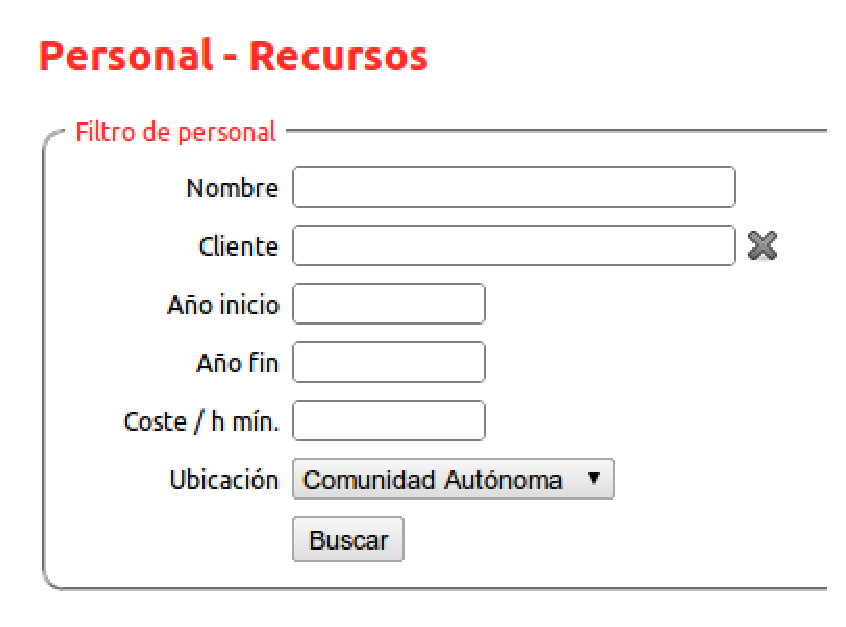
\epsfig{file=imagenes/filtro_personal,width=3.5in}
\caption{Detalle del filtro de personal.}
\label{fig:detalle_filtro_personal}
\end{figure}

En las especificaciones, se ha insistido en la necesidad de facilitar al máximo
la labor de búsqueda de información. La imagen \ref{fig:detalle_filtro_personal}
muestra un detalle del filtro de personal. Se aprecia el uso de cajas de texto
para casi todos los campos, exceptuando la caja de selección de Comunidad
Autónoma. Podría argumentarse que la selección de cliente también es susceptible
de implementarse por medio de una caja de selección, pero se tomó la decisión de
crear un sistema de sugerencias para la selección de clientes, implementado
haciendo uso de AJAX, como se verá en el capítulo \ref{chp:implementacion}. La
motivación para esta decisión no es otra que el elevado y creciente número de
clientes de Ingeniería e Innovación. A fecha de creación de esta memoria, el
número de clientes registrados es de 214, por lo que el uso de una caja de
selección típica resulta demasiado pesado para el usuario, que se vería forzado
a navegar por la lista cada vez que quisiera seleccionar un cliente. La barra de
desplazamiento de la imagen \ref{fig:seleccion_cliente_old} (difuminada
intencionadamente) puede dar una idea
de lo larga que es esa lista y la incomodidad que puede causar al usuario.

\begin{figure}
\centering
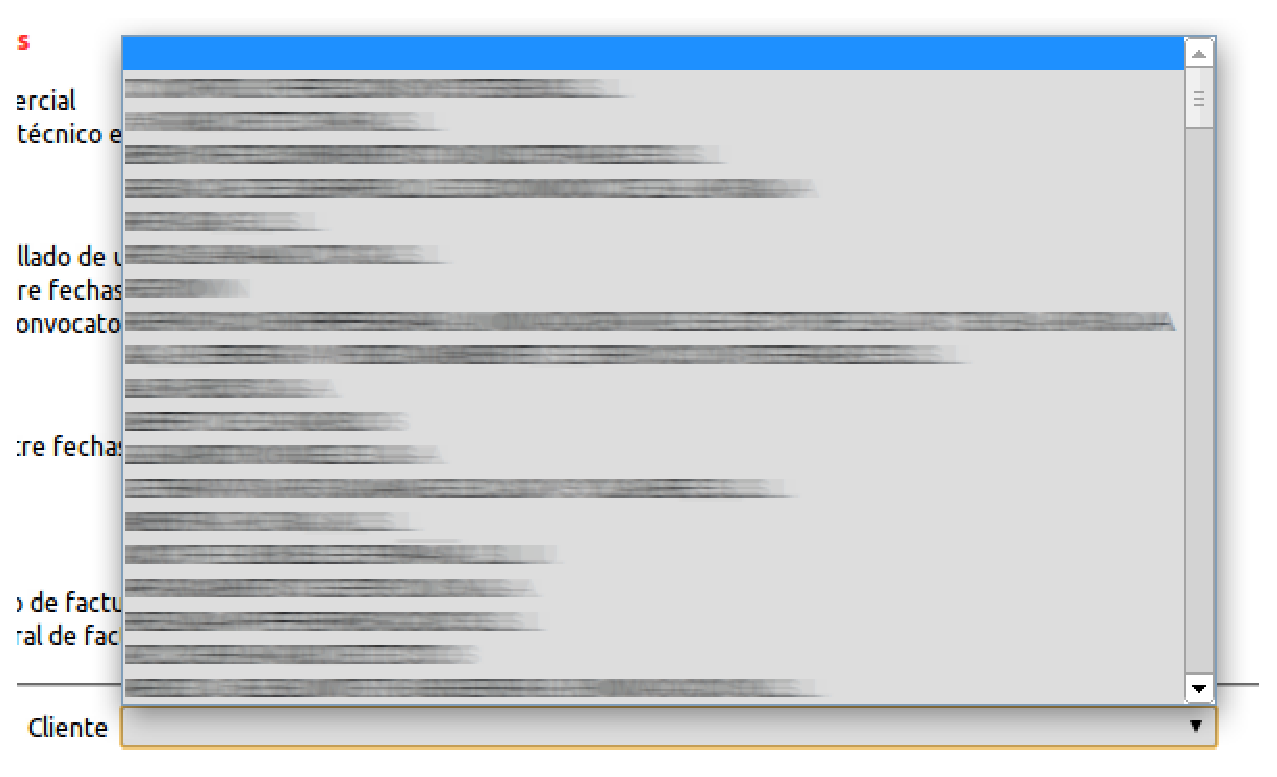
\epsfig{file=imagenes/seleccion_cliente_old,width=5in}
\caption{Selección de cliente mediante caja de selección.}
\label{fig:seleccion_cliente_old}
\end{figure}

El enfoque de las sugerencias, que se usará también en la selección de
proyectos (392 hasta el momento y creciendo), está cada vez más presente en muy
diversos ámbitos de la web (sirva como ejemplo la figura
\ref{fig:sugerencias_web}), ya que ofrece varias ventajas respecto al otro
sistema:

\begin{itemize}
 \item Elimina la necesidad de mostrar toda la lista, que es muy grande y
podría ralentizar la descarga de la página.
 \item Facilita y acelera la búsqueda: cuando el usuario ha introducido tres o
cuatro letras, ya obtiene los resultados esperados.
 \item Es muy versátil: en el caso de los proyectos,
el usuario puede buscarlos por nombre, acrónimo, cliente y acrónimo de cliente.
\end{itemize}


\begin{figure}
\centering
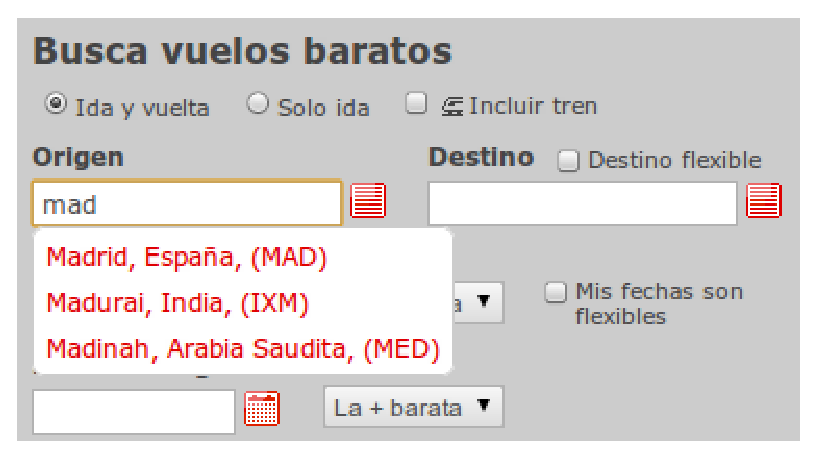
\epsfig{file=imagenes/sugerencias_web,width=3in}
\caption{Sugerencias de aeropuerto en un portal de vuelos.}
\label{fig:sugerencias_web}
\end{figure}

Los formularios están creados usando las mismas estructuras que los ya
existentes, de modo que la experiencia es siempre la misma. La figura
\ref{fig:comparacion_formularios} muestra una comparación entre un formulario
nuevo y uno ya existente.

\begin{figure}
\centering
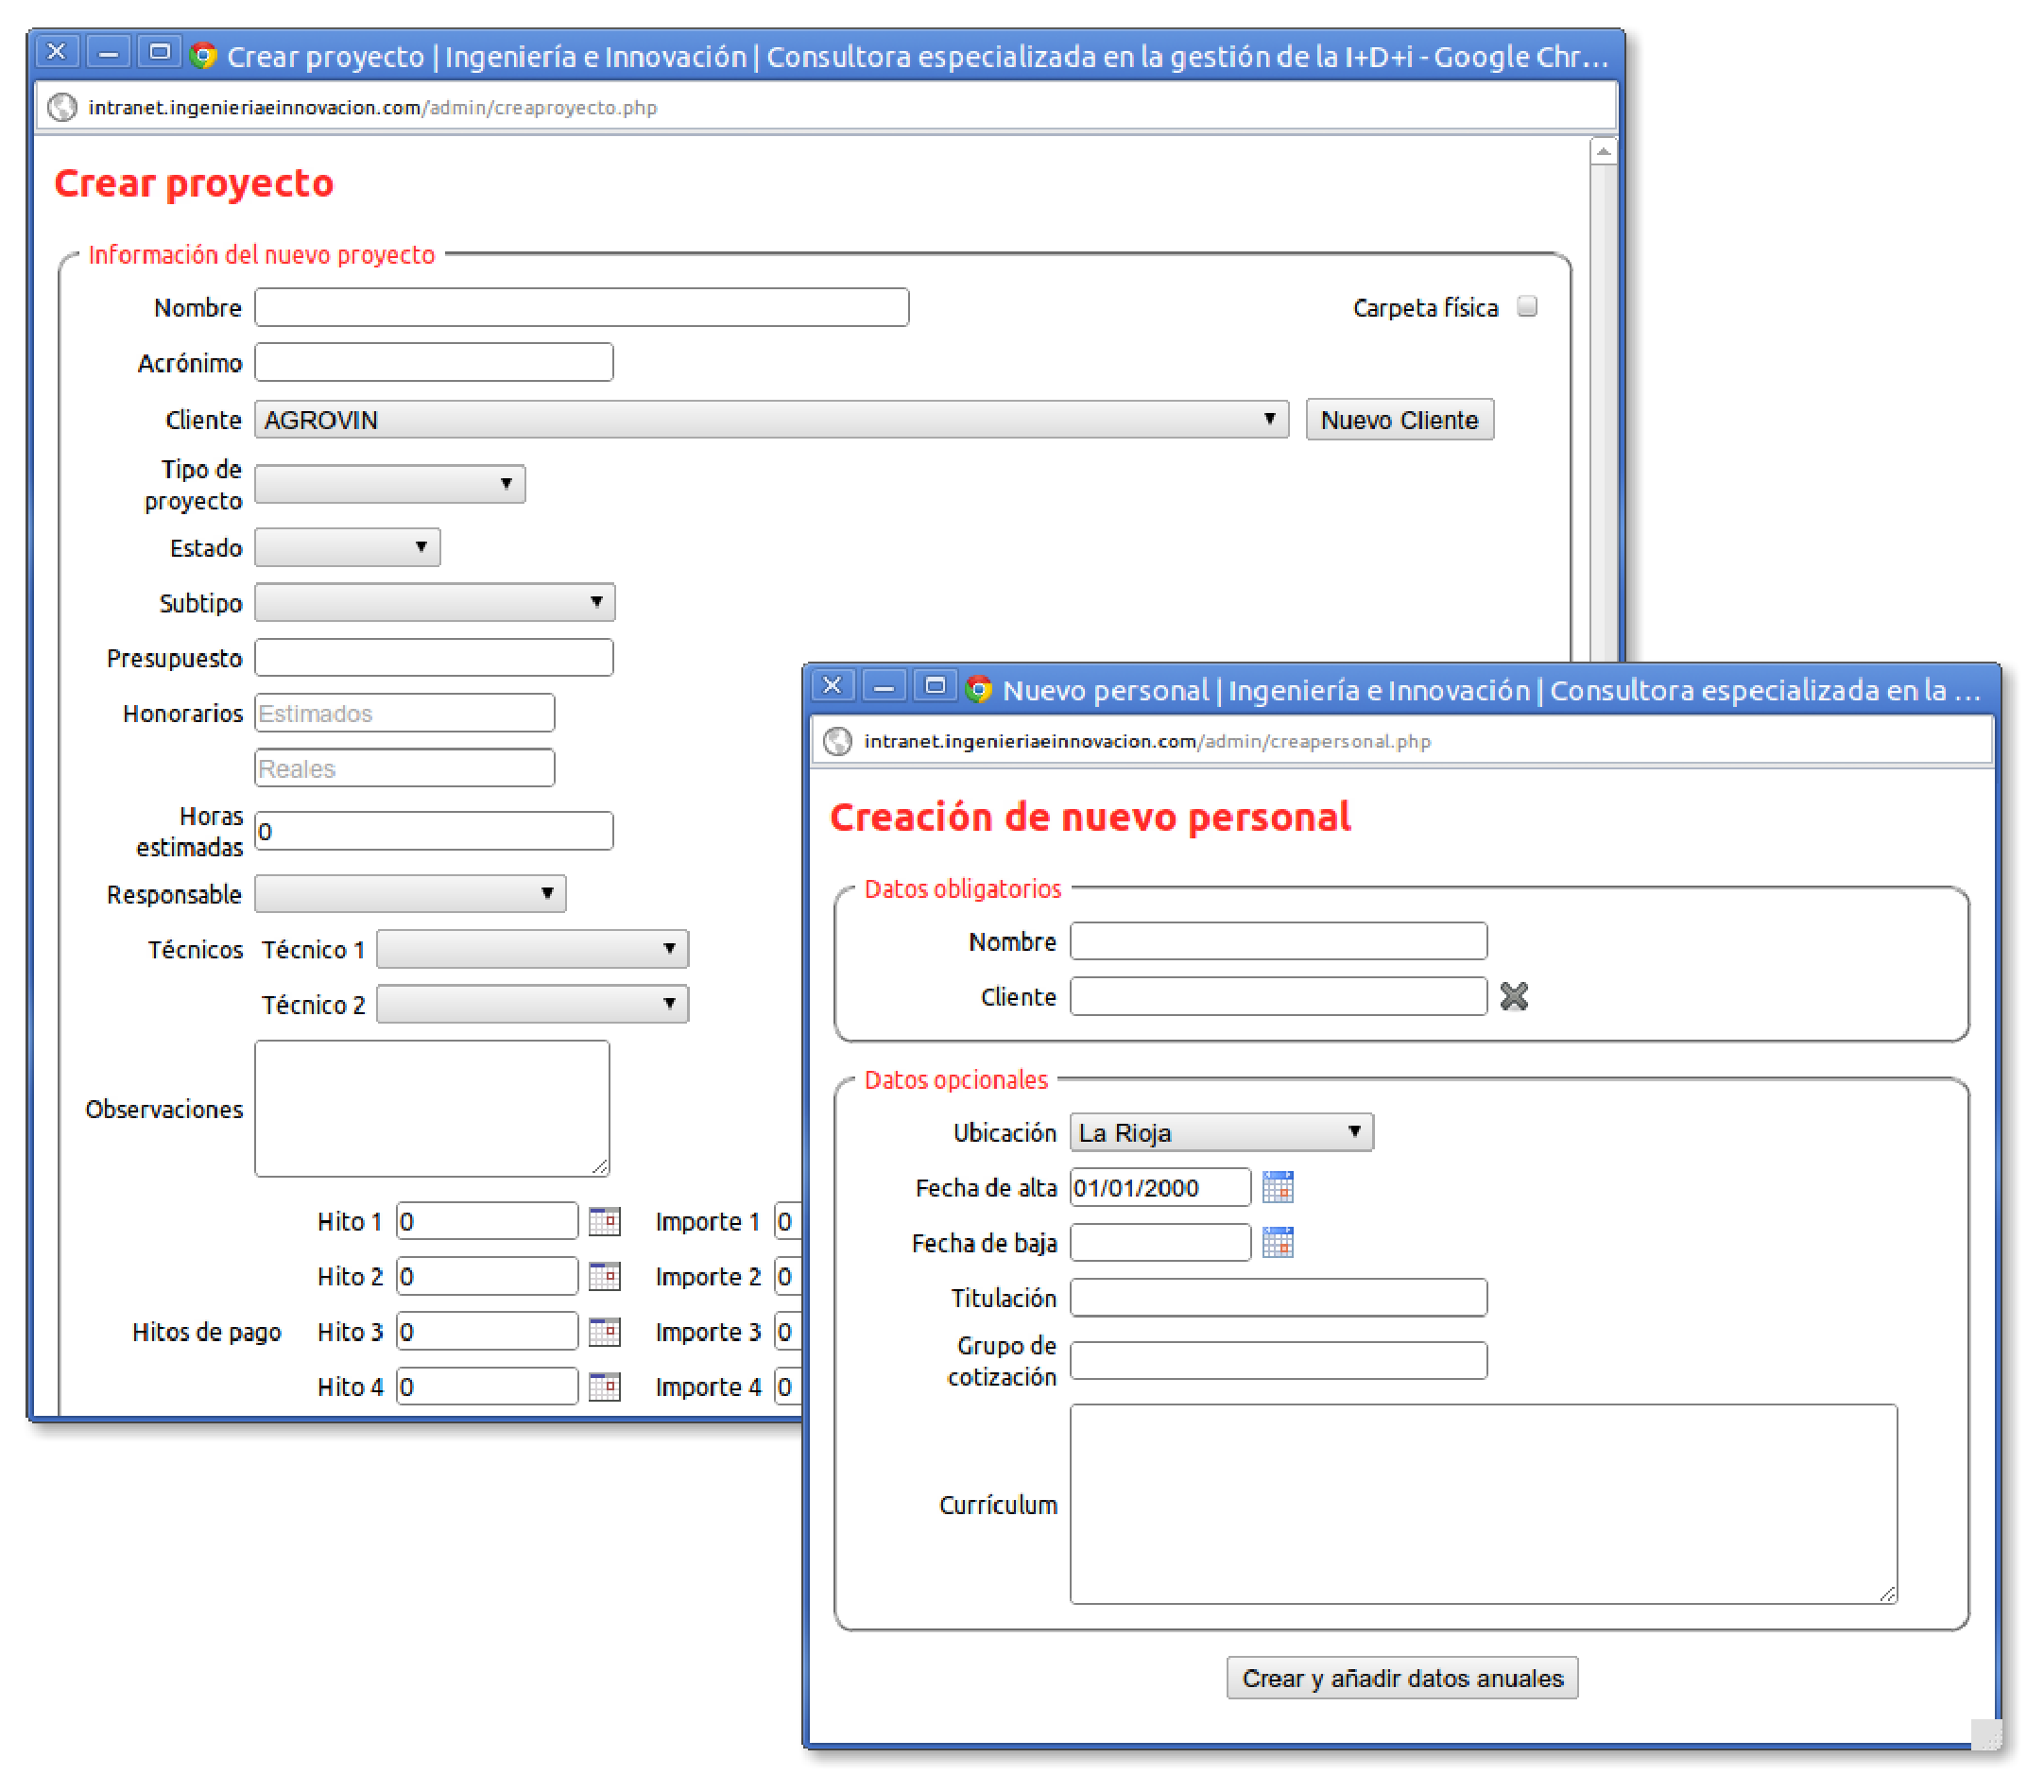
\epsfig{file=imagenes/comparacion_formularios,width=5.28in}
\caption{Formulario existente (izq.) frente a formulario nuevo (dcha.).}
\label{fig:comparacion_formularios}
\end{figure}

En la figura \ref{fig:comparacion_formularios} puede apreciarse otra decisión
tomada en favor de la usabilidad de la interfaz: en lugar de marcar los campos
obligatorios en negrita o con un asterisco, estos se encuentran
físicamente separados en su propio \textit{fieldset} con la etiqueta «Datos
obligatorios».

\subsection{Tablas}

La herramienta está plagada de tablas: se usan para mostrar los registros
anuales de los recursos humanos, para mostrar las actividades de cada proyecto,
en el detalle mensual de horas...

En la figura \ref{fig:tablas} se comprueba que se han intentado tratar de
la misma manera, para que la experiencia sea consistente.

\begin{figure}
\centering
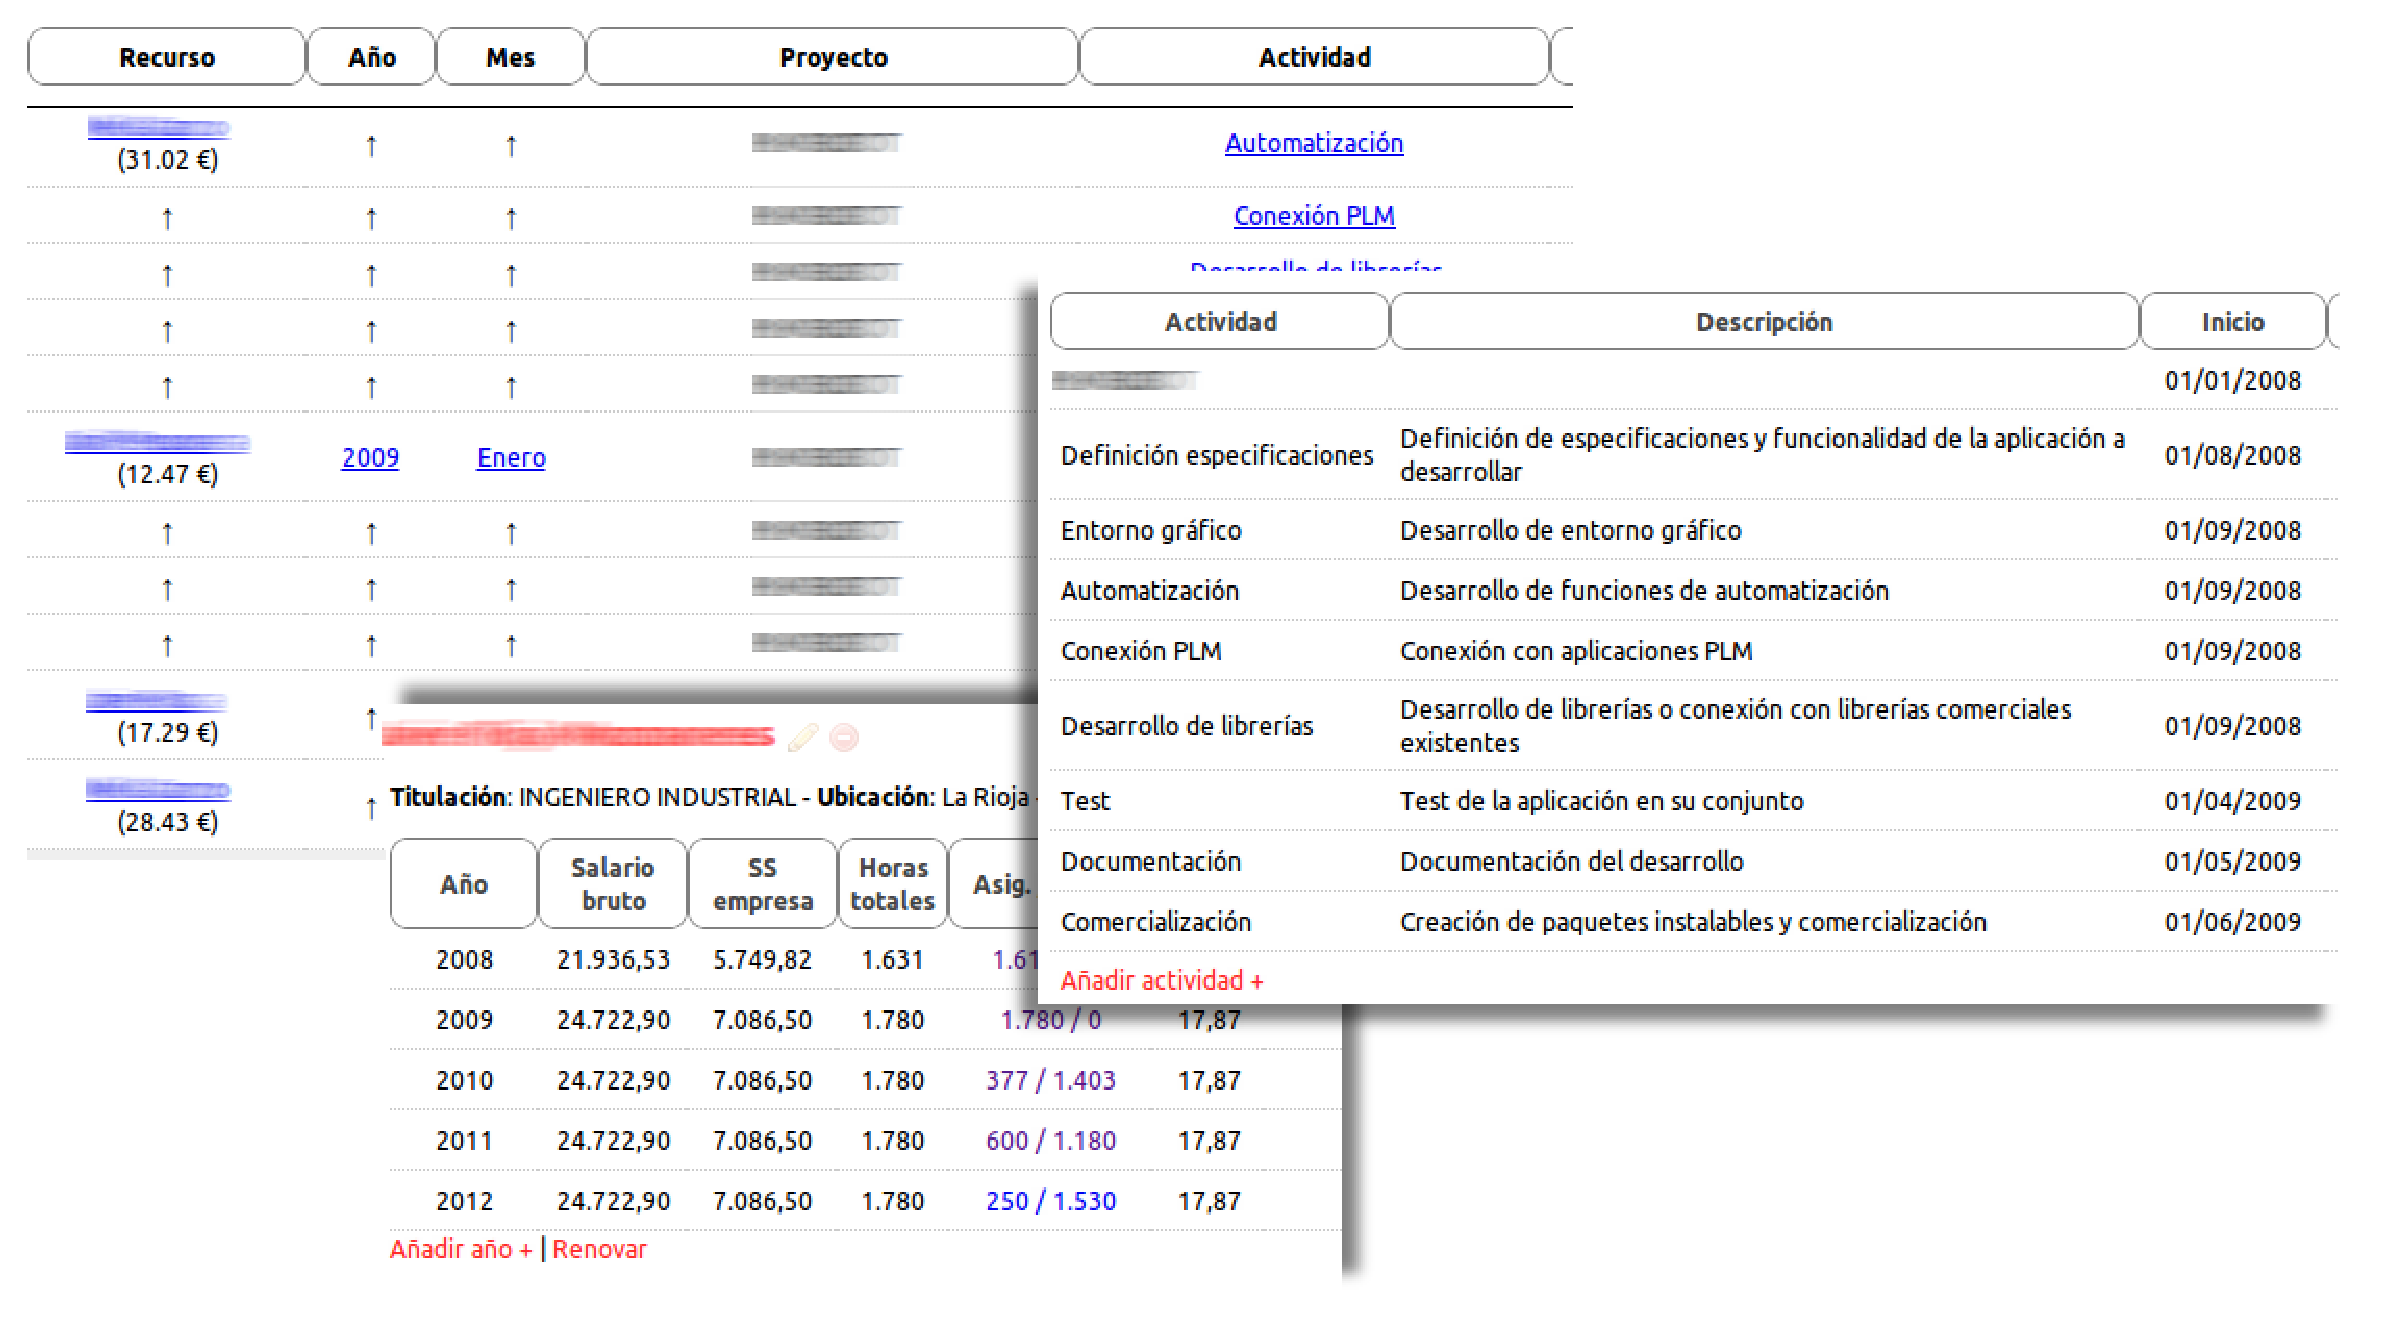
\epsfig{file=imagenes/tablas,width=5.28in}
\caption{Varias tablas de la herramienta.}
\label{fig:tablas}
\end{figure}

Una característica interesante es que se ha incluido en las tablas la capacidad
de ordenarlas pinchando en la cabecera de cada columna, al estilo de las
aplicaciones de escritorio. En el capítulo \ref{chp:implementacion} se hará
referencia a esta cualidad, lograda por medio de una librería externa.

\begin{figure}
\centering
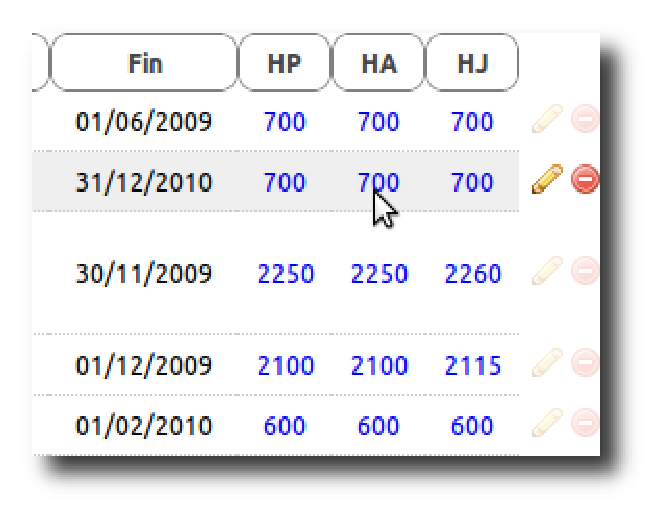
\epsfig{file=imagenes/detalle_tabla,width=3in}
\caption{Detalle de fila activa en una tabla.}
\label{fig:detalle_tabla}
\end{figure}

También, como segunda decisión de importancia tomada acerca de las tablas, la
fila sobre la que está el cursor se resalta con un fondo gris y las opciones de
modificación, eliminación..., que son semitransparentes, se hacen opacas, como
se puede apreciar en la figura \ref{fig:detalle_tabla}.

Como se puede ver en las imágenes mostradas, se ha intentado que
las tablas sean limpias y claras mostrando únicamente los bordes inferiores de
cada fila, evitando el uso de \textit{colspans} y, en general, evitando el uso
de tablas para datos que no sean tabulares, en contraposición a otras tablas
presentes en la aplicación global, que han demostrado ser confusas y difíciles
de mantener (ver figura \ref{fig:tabla_antigua}).

Finalmente, las tablas están llenas de enlaces: a detalles de horas,
información de recursos... En este sentido, se decidió no dar formato a los
enlaces, de modo que siguen la convención habitual, azules los no visitados,
morados los visitados. Los iconos, por su parte, están tomados de otras partes
de la aplicación global, para mantener la consistencia.

\begin{figure}
\centering
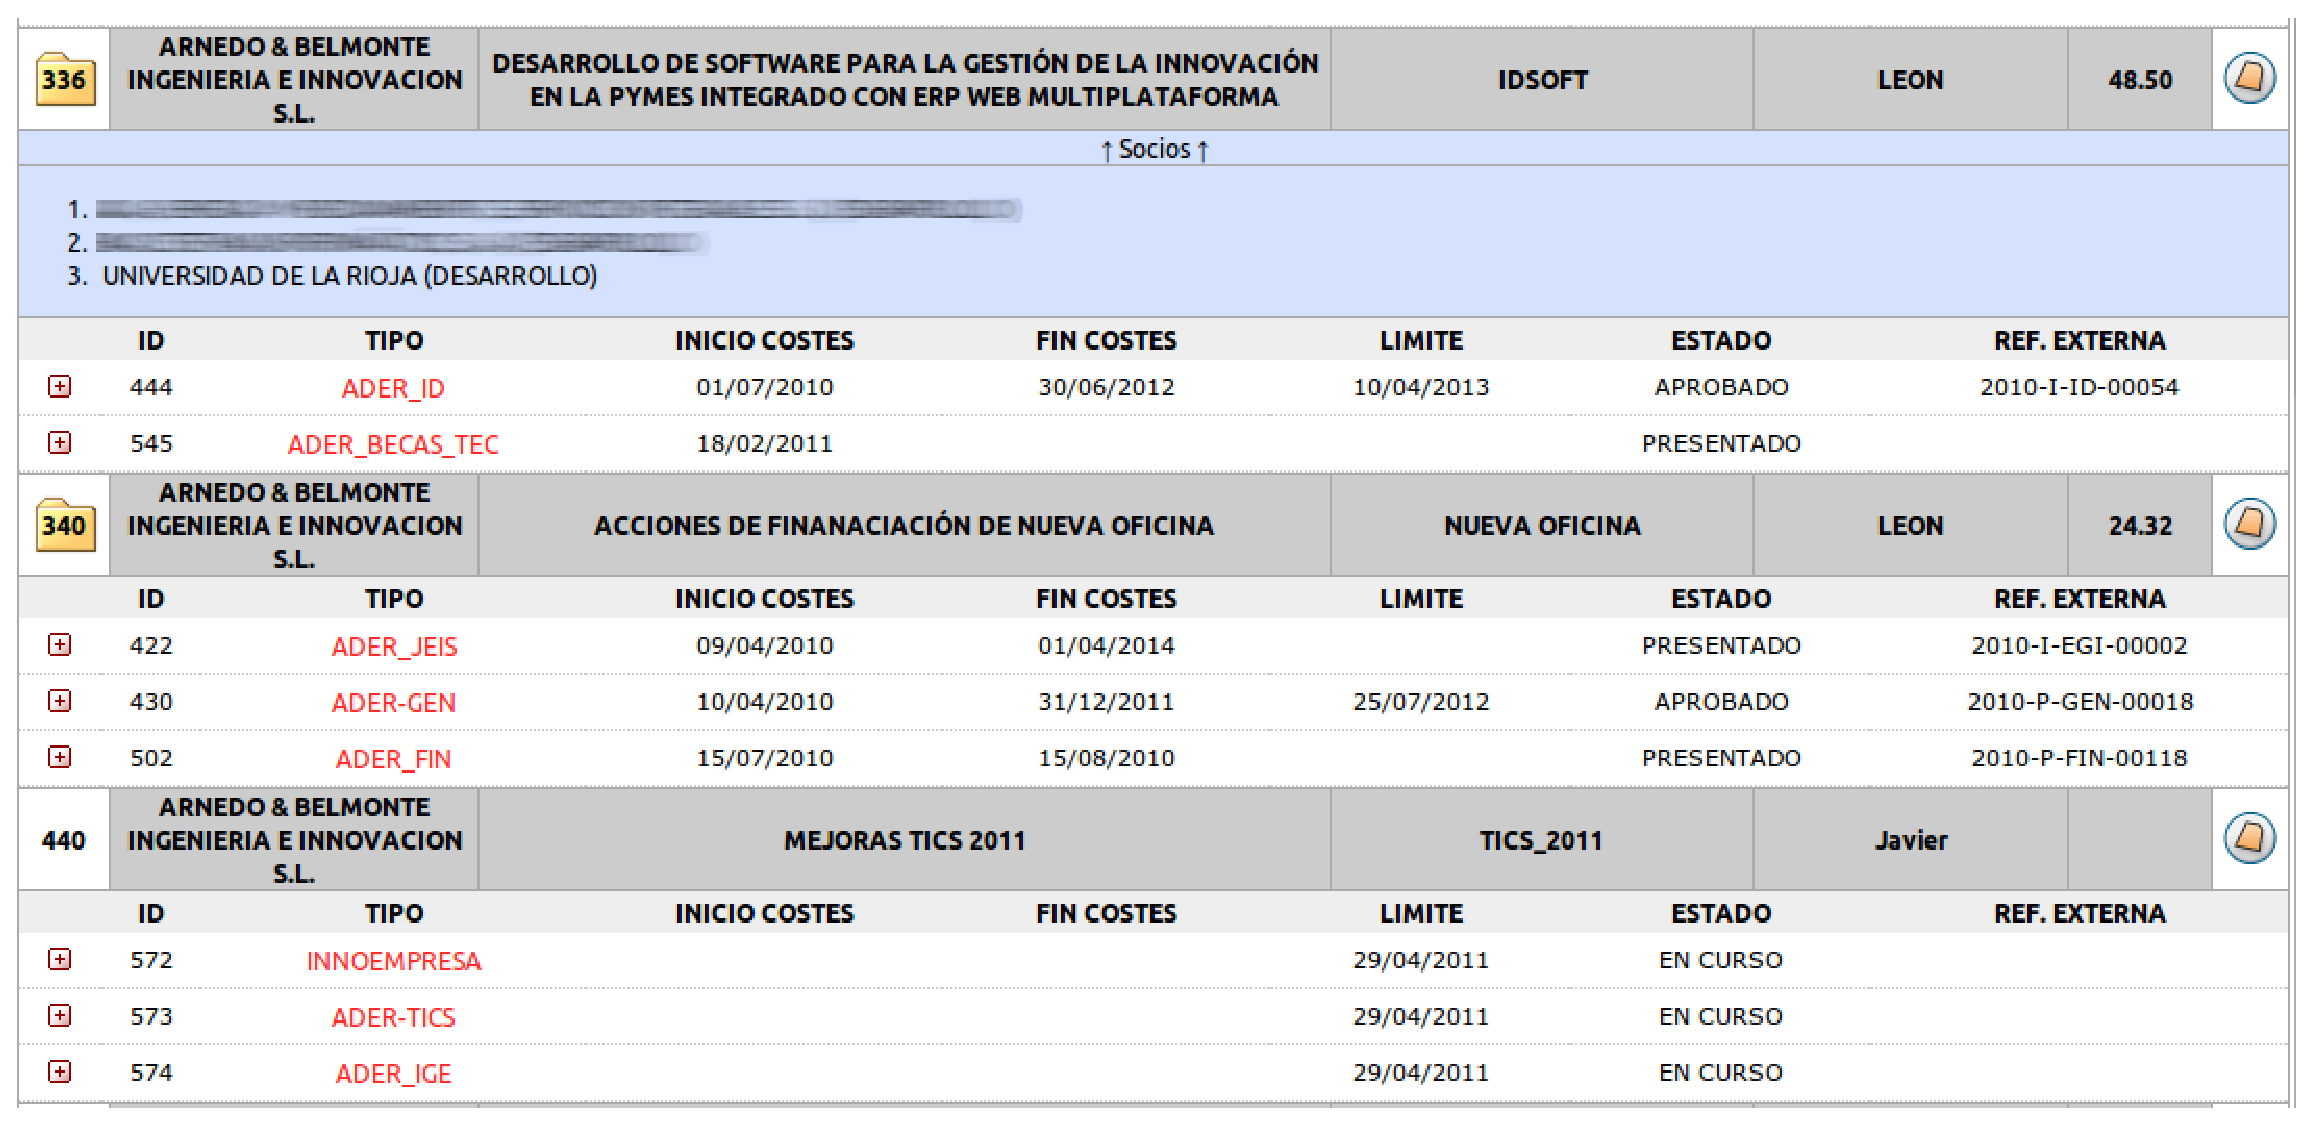
\epsfig{file=imagenes/tabla_antigua,width=5.28in}
\caption{Tabla antigua.}
\label{fig:tabla_antigua}
\end{figure}

\subsection{Ventanas emergentes}

La interacción con la herramienta incluye multitud de ventanas emergentes, en
consonancia con las partes preexistentes: se usan para crear personal y
actividades, asignar horas, modificar entidades...

El proyectante, conocedor de la tendencia a prescindir de este tipo de
interacción a la hora de diseñar interfaces, ha probado el uso de
\textit{lightboxes} en otras partes de la aplicación menos relevantes, pero
hasta que no se tome la decisión de abandonar el método de las ventanas
emergentes de forma completa, se ha decidido seguir de esta manera.

Una ventaja de las ventanas emergentes es que muchas veces se necesita
información de la ventana previa para rellenar el formulario de
creación/modificación oportuno, y estas ventanas lo consiguen independizándose
totalmente. Sin embargo, rompen la tónica habitual de lo que debería ser una
experiencia fluida y muchos usuarios acaban teniendo infinidad de ventanas
emergentes porque no se dan cuenta de que ya tenían una y siguen abriendo. Las
\textit{lightboxes} son una clase muy particular de elemento dentro de la propia
página que centra la atención del usuario sin romper la experiencia, y en muchos
casos, dejando la mayor parte de la vista original visible (aunque a veces
atenuada para captar la atención del usuario), como se aprecia en la figura
\ref{fig:ventana_modal}.

\begin{figure}
\centering
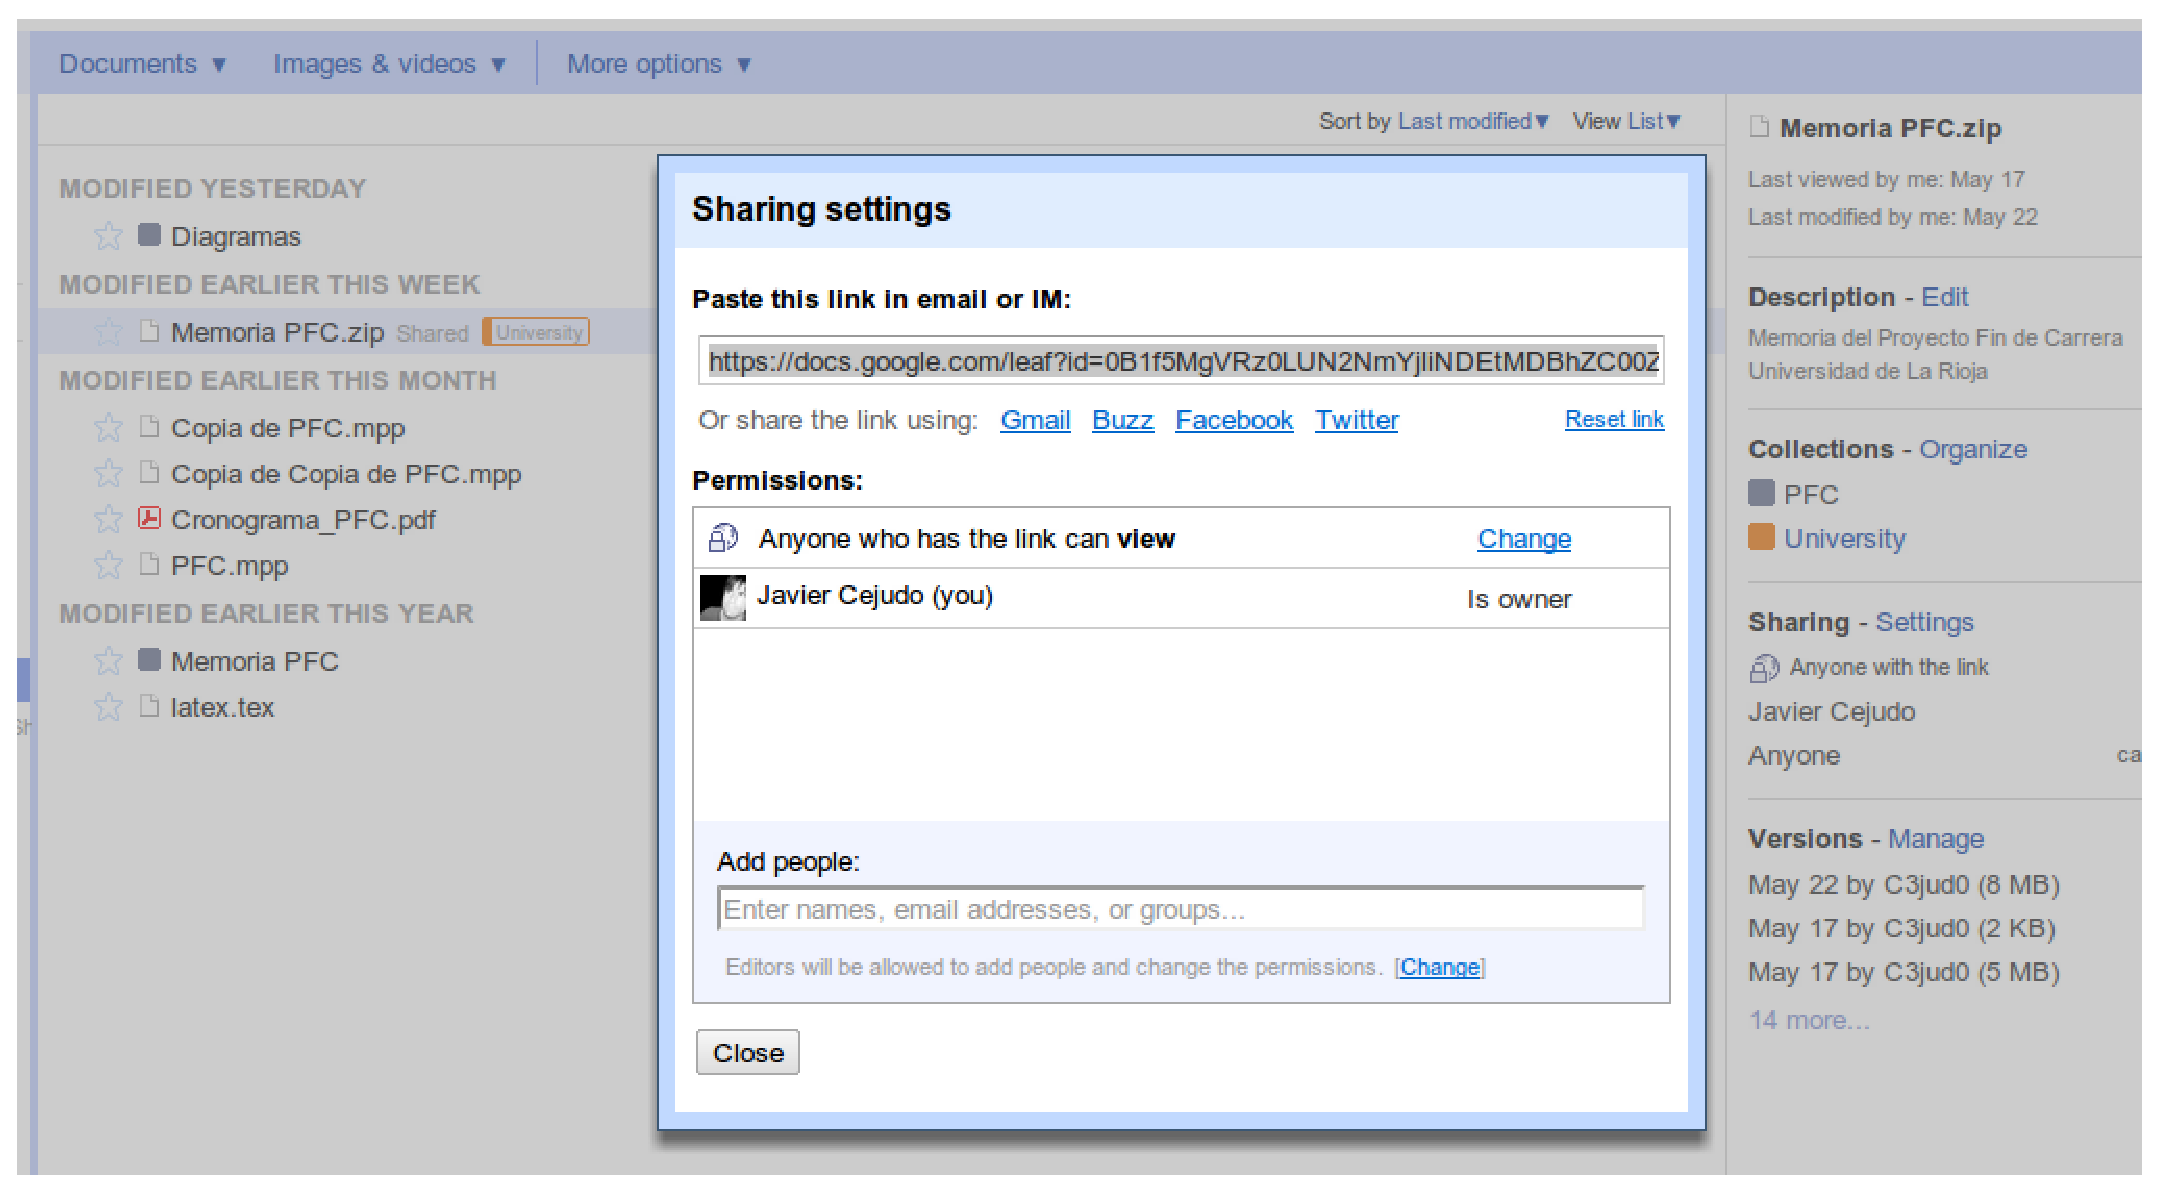
\epsfig{file=imagenes/ventana_modal,width=5.28in}
\caption{Ejemplo de lightbox en Google Docs.}
\label{fig:ventana_modal}
\end{figure}

\subsection{Buscador global}

\begin{figure}
\centering
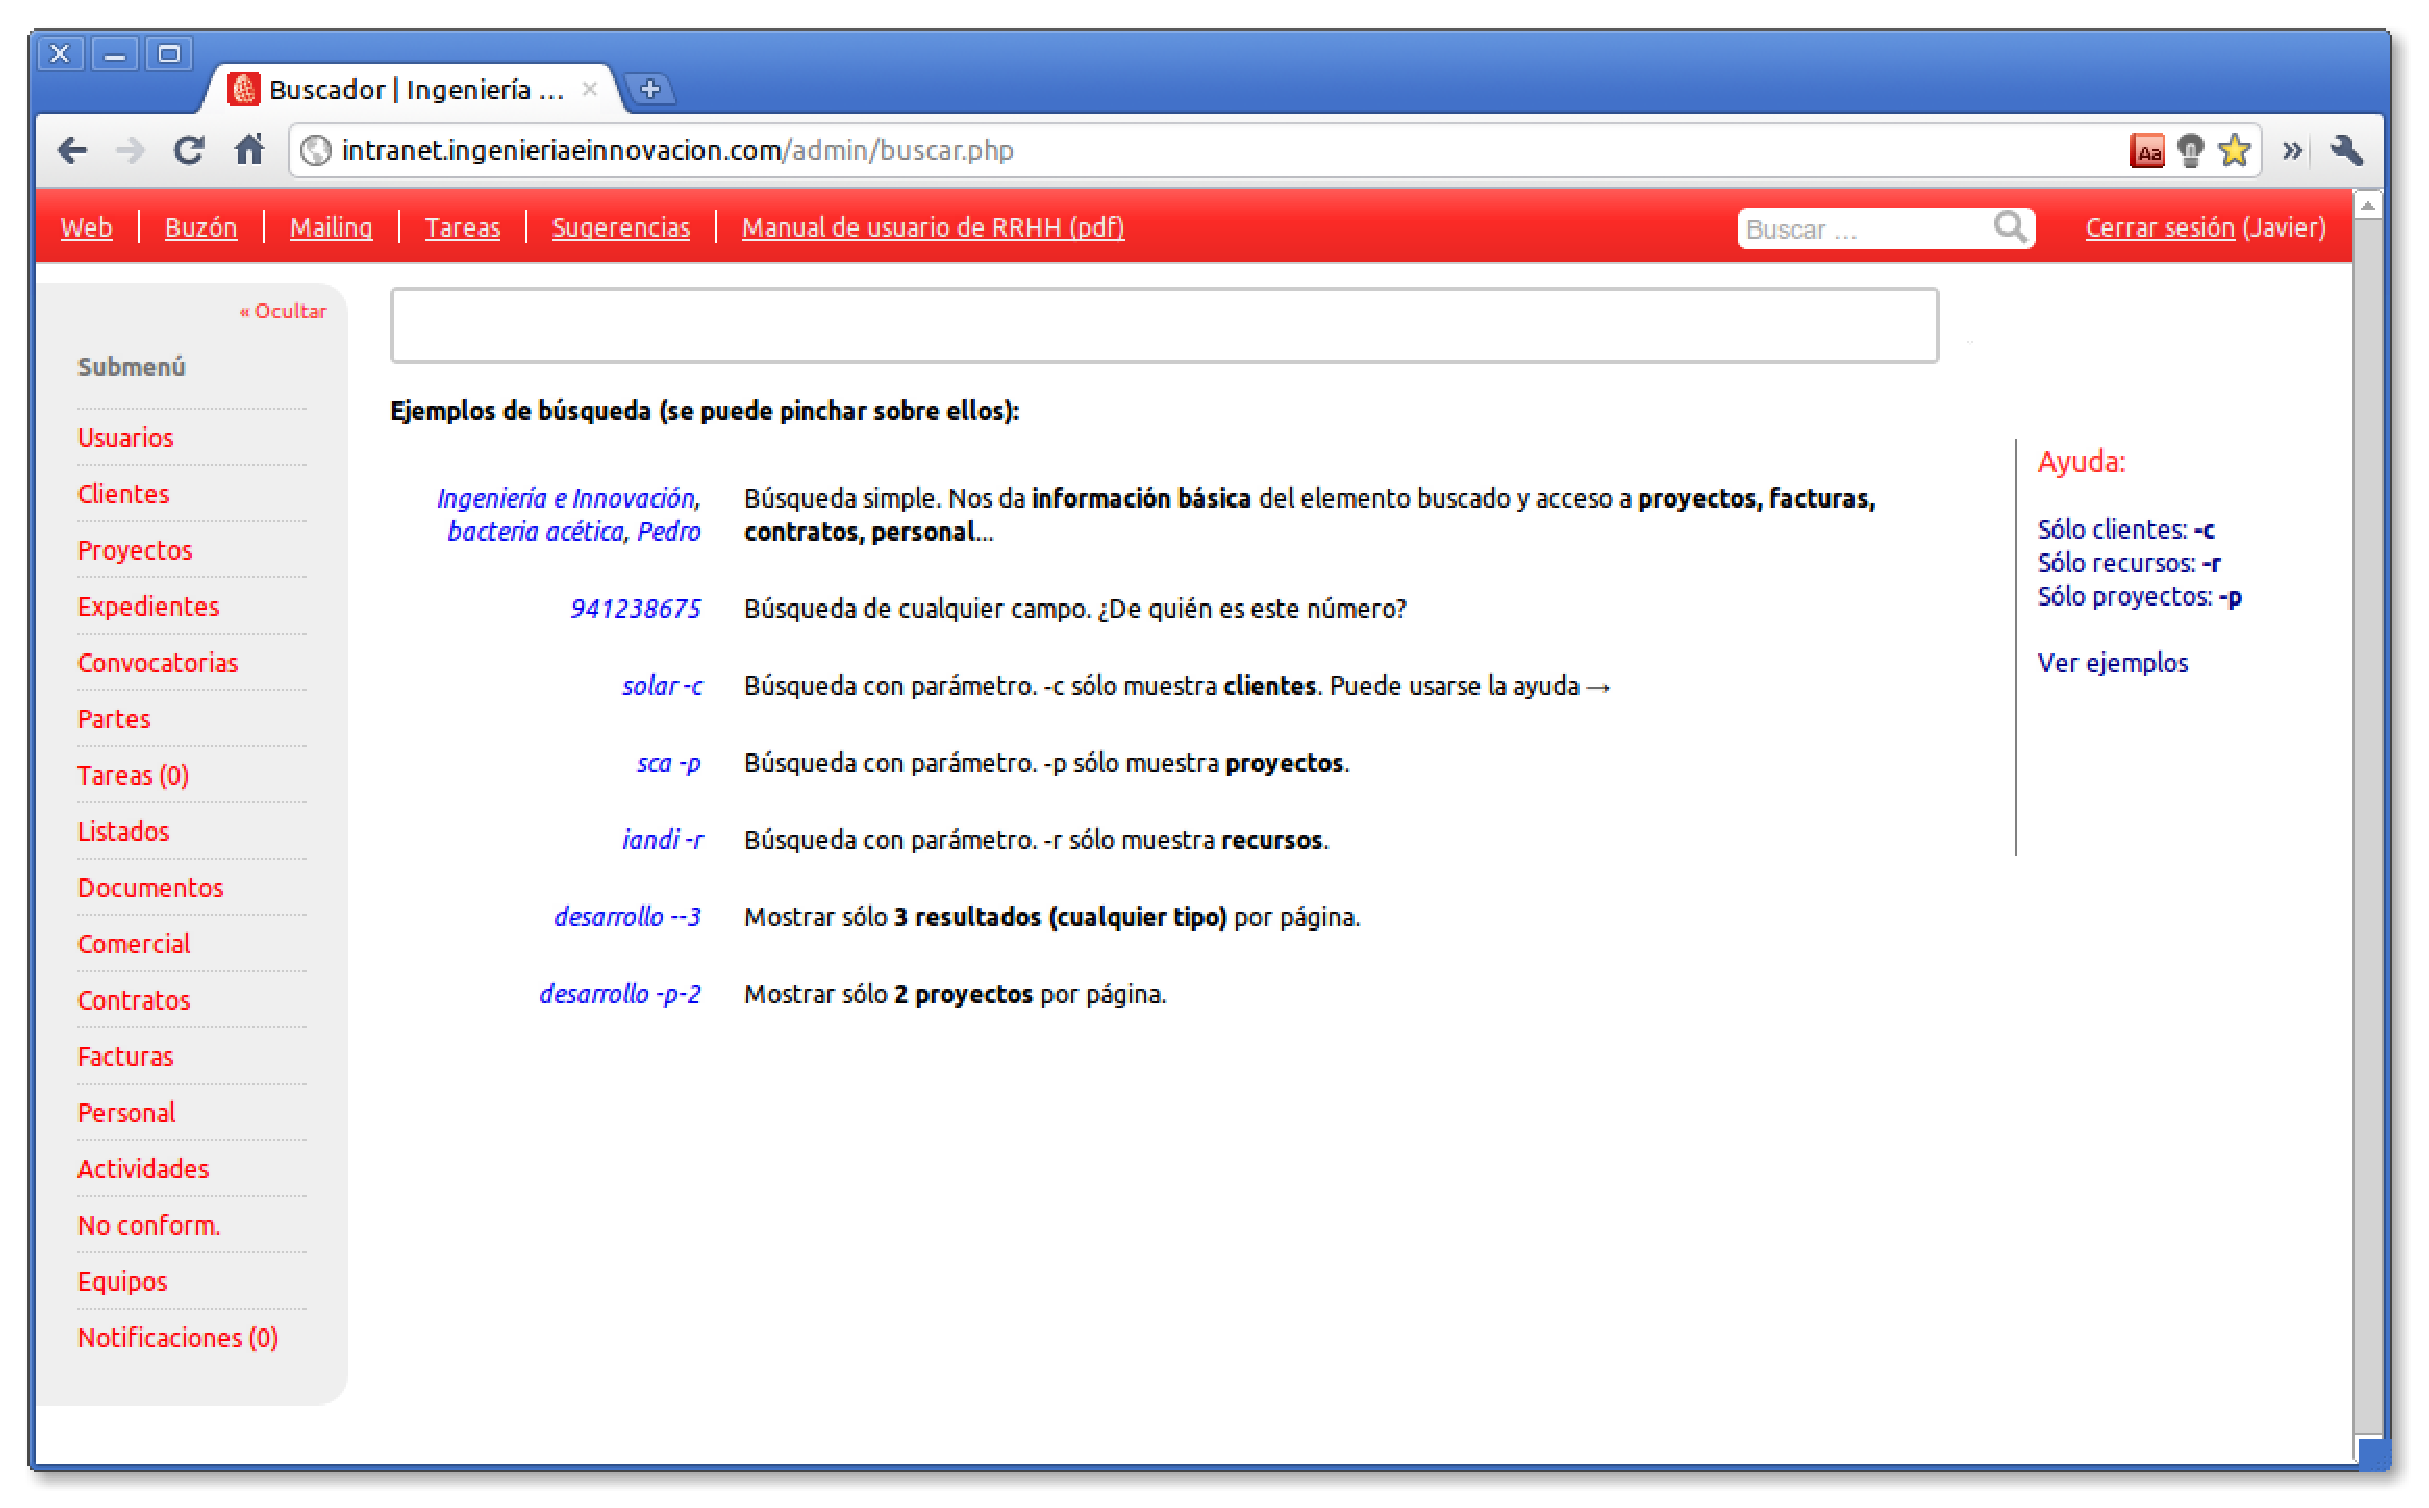
\epsfig{file=imagenes/buscador_inicio,width=5.28in}
\caption{Buscador global.}
\label{fig:buscador_inicio0}
\end{figure}

El buscador, al ser una herramienta nueva y diferenciada del resto de la
aplicación, ha requerido un mayor número de decisiones de cara a su diseño.

En primer lugar, muestra una serie de ejemplos, desde los más simples hasta
ejemplos más avanzados, de modo que estén a mano en cualquier momento y los
usuarios se familiaricen con ellos. Estos ejemplos están brevemente explicados y
son interactivos, de manera que pinchando en ellos veremos el tipo de resultados
que proporcionan.

Los colores empleados son los corporativos, pero la estructura de los resultados
es muy similar a la de los buscadores generalistas (véase la figura
\ref{fig:resultado_busqueda}): título, descripción, datos adicionales y otros
enlaces de interés.

\begin{figure}
\centering

\epsfig{file=imagenes/resultado_busqueda,width=5.28in}
\caption{Detalle de un resultado.}
\label{fig:resultado_busqueda}
\end{figure}

La paginación funciona, también, como en cualquier otro buscador: enlaces a las
páginas siguientes, a las anteriores, marcado de página actual, y enlace
siempre visible a la primera y última página, para dar contexto. Dada la
naturaleza instantánea del buscador, se han seguido las convenciones do Google
Instant: cada vez que el buscador está cargando, los resultados se vuelven
semitransparentes (figura \ref{fig:buscador_cargando}), y en el caso de cambio
de página, la barra de desplazamiento se posiciona al principio de los
resultados.

\begin{figure}
\centering
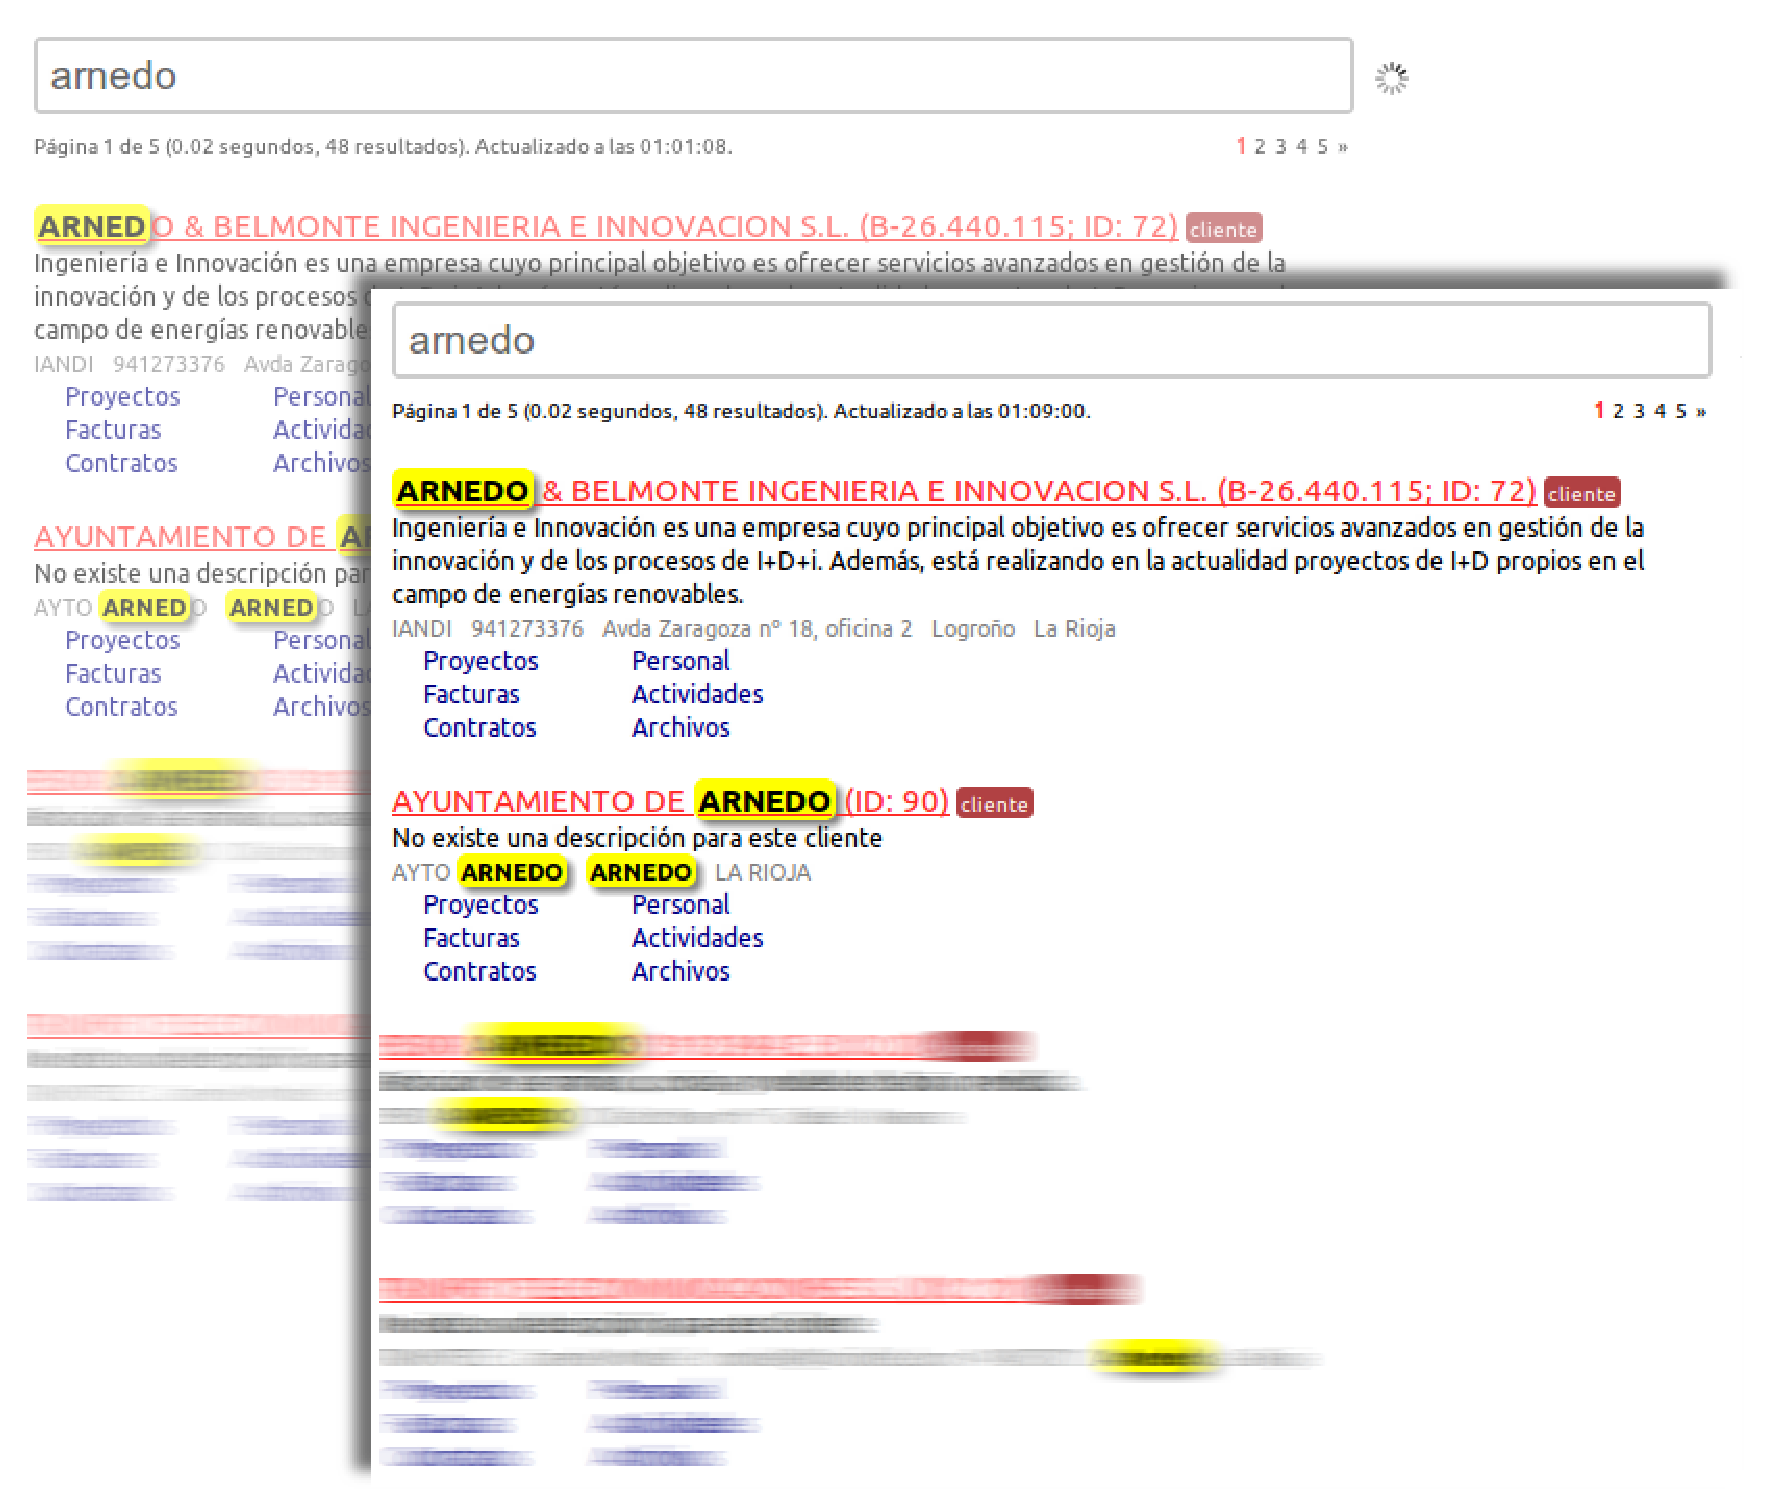
\epsfig{file=imagenes/buscador_cargando,width=5.28in}
\caption{Buscador cargando (izq.) y estado normal (dcha.)}
\label{fig:buscador_cargando}
\end{figure}

La última característica que requiere mención especial es que se permite la
navegación por teclado, de modo que la flecha derecha ($\rightarrow$) pasa a la
siguiente página y la flecha izquierda ($\leftarrow$), a la anterior.

\section{Diseño de la base de datos}

Como ya se ha mencionado anteriormente, se ha empleado una base de datos
relacional gestionada por MySQL. En esta sección, pueden encontrarse los
detalles acerca de las entidades, sus atributos, y las relaciones que se
establecen entre ellas.

Debe notarse que si bien se ha intentado hacer un diseño razonable que no
utilice recursos innecesarios, no se ha llevado a cabo un proceso de
normalización. En los siguientes párrafos se explicará brevemente
la motivación y las decisiones tomadas acerca de los aspectos más relevantes
relacionados con el diseño de la base de datos.

\subsection{Diagrama Entidad/Relación}

En el diagrama de Entidad/Relación (figura \ref{fig:ERD}) puede verse de forma
rápida las entidades involucradas y la forma en que se relacionan entre ellas.
Se han incluido las entidades preexistentes PROYECTO y CLIENTE, ya que
están relacionadas con las nuevas entidades que introduce la herramienta que nos
ocupa. Nótese que, por simplicidad, no se han incluido en este diagrama los
atributos que registran la creación y modificación de los datos.

\begin{figure}
\centering
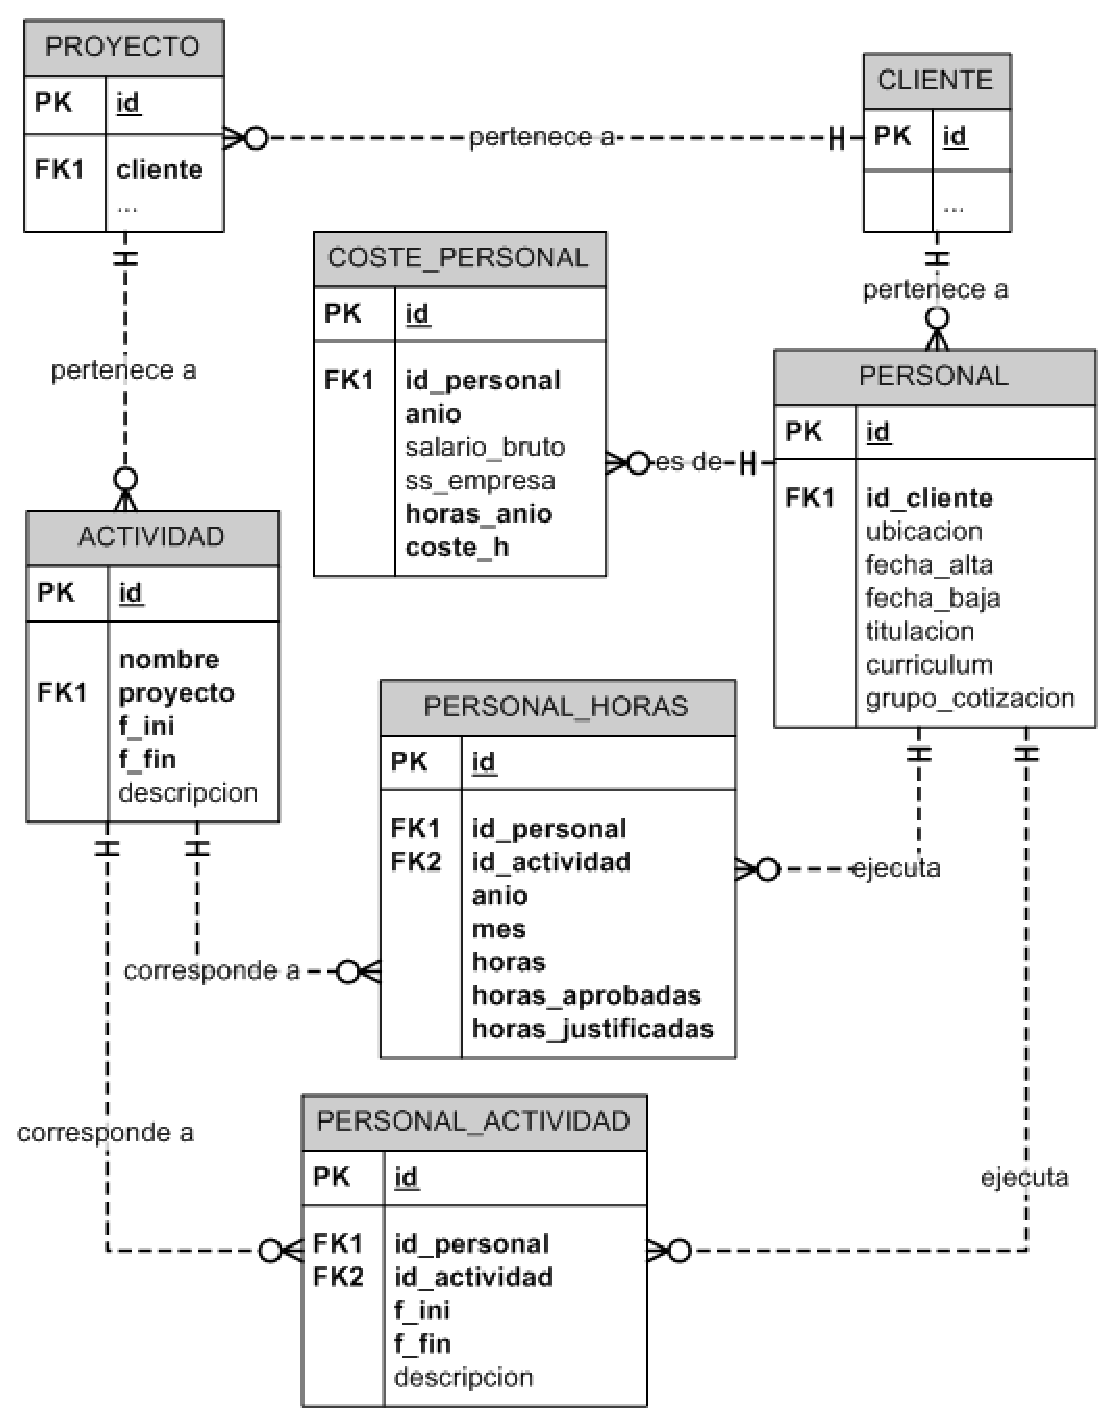
\epsfig{file=imagenes/ERD,width=5.28in}
\caption{Diagrama E--R}
\label{fig:ERD}
\end{figure}

\subsection{Entidades y atributos}

En el cuadro \ref{tab:tablas_atributos} se muestra un resumen de las nuevas
entidades creadas.

Nótese que algunos atributos hacen referencia a entidades preexistentes, como se
explicará en la sección \ref{sec:relaciones}.

\begin{table}
\small
\centering
\begin{tabular}{|l|p{3in}|}\hline
\textbf{Nombre} & \textbf{Atributos}\\\hline\hline
\textbf{ACTIVIDAD} & id, nombre,
    proyecto, f\_ini, f\_fin, descripcion, fecha\_creacion, usu\_creacion,
    fecha\_modificacion, usu\_modificacion\\\hline
\textbf{COSTE\_PERSONAL} & id, id\_personal, anio, salario\_bruto, ss\_empresa,
    coste\_h, horas\_anio, usuario\_creacion, fecha\_creacion, usuario\_act,
    fecha\_act\\\hline
\textbf{PERSONAL} & id, id\_cliente, ubicacion, nombre, fecha\_alta,
    fecha\_baja,    titulacion, curriculum, grupo\_cotizacion, fecha\_creacion,
    usu\_creacion,    fecha\_modificacion, usu\_modificacion \\\hline
\textbf{PERSONAL\_ACTIVIDAD} & id, id\_personal, id\_actividad, f\_ini, f\_fin,
    descripcion, fecha\_creacion, usu\_creacion, fecha\_modificacion,
    usu\_modificacion \\\hline
\textbf{PERSONAL\_HORAS} & id, id\_personal, id\_actividad, anio, mes, horas,
    horas\_aprobadas, horas\_justificadas, fecha\_creacion, usu\_creacion,
    fecha\_modificacion, usu\_modificacion \\\hline
\end{tabular}
\caption{Atributos de las entidades creadas}
\label{tab:tablas_atributos}
\end{table}

La tabla ACTIVIDAD (cuadro \ref{tab:tabla_actividad}) recogerá la información
relacionada con las actividades: su nombre, a qué proyecto pertenecen, fechas
de inicio y finalización y descripción. De manera automática, se recogerán
datos relativos a la creación y modificación de las actividades, de manera que,
en caso de errores o inconsistencias, se pueda recuperar cuándo se produjeron y
quién la introdujo para facilitar la corrección.

\begin{table}
\small
\centering
\begin{tabular}{|l|p{2in}|l|l|}\hline
\textbf{Atributo} & \textbf{Descripción} & \textbf{Tipo de dato} &
\textbf{Nulo} \\\hline\hline
id & identificador autoincremental & INT(11) & No\\\hline
nombre & nombre de la actividad & VARCHAR(255) & No\\\hline
proyecto & identificador del proyecto al que pertenece & INT(11) & No\\\hline
f\_ini & fecha de inicio aproximada & INT(11) & No\\\hline
f\_fin & fecha de fin aproximada & INT(11) & No\\\hline
descripcion & descripcion extensa & TEXT & Sí\\\hline
fecha\_creacion & registro automático de la fecha de creación & INT(11) &
No\\\hline
usuario\_creacion & registro automático del usuario creador & INT(11) &
No\\\hline
fecha\_modificacion & registro automático de la fecha de creación & INT(11) &
Sí\\\hline
usuario\_modificacion & registro automático del usuario modificador & INT(11) &
Sí\\\hline
\end{tabular}
\caption{Atributos de la tabla ACTIVIDAD}
\label{tab:tabla_actividad}
\end{table}

La tabla PERSONAL (cuadro \ref{tab:tabla_personal}) recogerá la información
relacionada con los empleados: su nombre, a qué cliente corresponden,
ubicación, fechas de alta y baja (si procede), titulación, currículum y grupo
de cotización. Las fechas de alta y baja no se han considerado obligatorias
debido a la falta de información al respecto que existe en muchos casos. Si se
conocen, la aplicación será capaz de detectar inconsistencias generadas de la
imputación de horas fuera de esas fechas. Idealmente, los clientes
proporcionarían toda la información relativa a los empleados, pero esto no es lo
común. Como en el caso anterior, se recogerán datos relativos a la creación y
modificación.

\begin{table}
\small
\centering
\begin{tabular}{|l|p{2in}|l|l|}\hline
\textbf{Atributo} & \textbf{Descripción} & \textbf{Tipo de dato} &
\textbf{Nulo} \\\hline\hline
id & identificador autoincremental & INT(11) & No\\\hline
id\_cliente & identificador del cliente al que hace referencia & INT(11) &
No\\\hline
ubicacion & CC.AA. en la que realiza su trabajo & INT(11) & Sí\\\hline
fecha\_alta & fecha de alta en la empresa & INT(11) & Sí\\\hline
fecha\_baja & fecha de baja en la empresa & INT(11) & Sí\\\hline
titulacion & titulación del empleado & VARCHAR(255) & Sí\\\hline
curriculum & currículum resumido del empleado & TEXT & Sí\\\hline
grupo\_cotizacion & grupo de cotización del empleado & VARCHAR(50) & Sí\\\hline
fecha\_creacion & registro automático de la fecha de creación & INT(11) &
No\\\hline
usuario\_creacion & registro automático del usuario creador & INT(11) &
No\\\hline
fecha\_modificacion & registro automático de la fecha de creación & INT(11) &
Sí\\\hline
usuario\_modificacion & registro automático del usuario modificador & INT(11) &
Sí\\\hline
\end{tabular}
\caption{Atributos de la tabla PERSONAL}
\label{tab:tabla_personal}
\end{table}

La tabla COSTE\_PERSONAL (cuadro \ref{tab:tabla_coste_personal}) recogerá la
información relacionada con los registros anuales. El nombre hace referencia al
coste hora del empleado porque este es uno de los datos fundamentales que van a
cambiar anualmente. Se guardan datos relativos al año al que se refiere el
registro, el salario bruto, el coste de Seguridad Social a cargo de la empresa
y el número de horas del convenio. Nótese que del salario bruto, el coste de
Seguridad Social a cargo de la empresa y las horas del convenio, se deduce el
coste hora del empleado, pero de nuevo, es muy común que en un principio no se
conozcan todos estos datos, o se proporcione solo alguno de ellos junto con el
coste hora final. En un caso ideal, podríamos prescindir del campo coste\_hora,
que sería deducido del resto. Como en los casos anteriores, se recogerán datos
relativos a la creación y modificación.

\begin{table}
\small
\centering
\begin{tabular}{|l|p{2in}|l|l|}\hline
\textbf{Atributo} & \textbf{Descripción} & \textbf{Tipo de dato} &
\textbf{Nulo} \\\hline\hline
id & identificador autoincremental & INT(11) & No\\\hline
id\_personal & identificador del empleado al que hace referencia & INT(11) &
No\\\hline
anio & año del registro anual & SMALLINT(4) & No\\\hline
salario\_bruto & salario bruto del empleado en el año & FLOAT(8,2) & Sí\\\hline
ss\_empresa & seguridad social a cargo de la empresa & FLOAT(8,2) & Sí\\\hline
horas\_anio & horas anuales según convenio & SMALLINT(4) & No\\\hline
coste\_h & coste por hora del empleado & FLOAT(4,2) & No\\\hline
fecha\_creacion & registro automático de la fecha de creación & INT(11) &
No\\\hline
usuario\_creacion & registro automático del usuario creador & INT(11) &
No\\\hline
fecha\_modificacion & registro automático de la fecha de creación & INT(11) &
Sí\\\hline
usuario\_modificacion & registro automático del usuario modificador & INT(11) &
Sí\\\hline
\end{tabular}
\caption{Atributos de la tabla COSTE\_PERSONAL}
\label{tab:tabla_coste_personal}
\end{table}

La tabla PERSONAL\_ACTIVIDAD (cuadro \ref{tab:tabla_personal_actividad})
recogerá la información relacionada con las asignaciones de horas realizadas.
Conviene subrayar que es información relacionada con la asignación, no la
asignación misma, ya que no guarda datos de horas. Se ha considerado
interesante conservar esta información, pero no sería estrictamente necesaria
tal y como se ha planteado la solución. En concreto, guarda las fechas exactas
de inicio y finalización del recurso en la actividad, que no tiene por qué
coincidir con las fechas de inicio y finalización de la actividad. Estas fechas
se usan en el reparto de horas, pero no se volverá a tener en cuenta más
adelante. También puede guardar la descripción de la labor del recurso en la
actividad. Se han incluido los datos de creación y modificación por si, en un
futuro, se implementase la capacidad de modificar asignaciones, posibilidad que
ahora es solventada mediante reasignaciones que se sobrescriben.

\begin{table}
\small
\centering
\begin{tabular}{|l|p{2in}|l|l|}\hline
\textbf{Atributo} & \textbf{Descripción} & \textbf{Tipo de dato} &
\textbf{Nulo} \\\hline\hline
id & identificador autoincremental & INT(11) & No\\\hline
id\_personal & identificador del empleado al que hace referencia & INT(11) &
No\\\hline
id\_actividad & identificador de la actividad a la que hace referencia & INT(11)
& No\\\hline
f\_ini & fecha de inicio del empleado en la actividad & INT(11) & No\\\hline
f\_fin & fecha de fin del empleado en la actividad & INT(11) & No\\\hline
descripcion & descripcion de su labor en la actividad & TEXT & Sí\\\hline
fecha\_creacion & registro automático de la fecha de creación & INT(11) &
No\\\hline
usuario\_creacion & registro automático del usuario creador & INT(11) &
No\\\hline
fecha\_modificacion & registro automático de la fecha de creación & INT(11) &
Sí\\\hline
usuario\_modificacion & registro automático del usuario modificador & INT(11) &
Sí\\\hline
\end{tabular}
\caption{Atributos de la tabla PERSONAL\_ACTIVIDAD}
\label{tab:tabla_personal_actividad}
\end{table}

La tabla PERSONAL\_HORAS (cuadro \ref{tab:tabla_personal_horas}) recogerá la
información relacionada con las horas asignadas. Dada la estructura de
concesión de ayudas a la I+D, se necesitan guardar horas presentadas, horas
aprobadas y horas justificadas. Una asignación genera tantos registros como
meses comprenda la duración de la labor del recurso en la actividad, de manera
que, en caso de haber considerado esencial la tabla PERSONAL\_ACTIVIDAD, habría
sido conveniente incluir un campo que hiciera referencia a la asignación a la
que originó cada registro; sin embargo, estos registros van a ser modificables
de manera individual, por lo que se ha decidido relacionar la tabla con el
personal y las actividades directamente. Evidentemente, los registros de esta
tabla están relacionados implícitamente con un solo registro de la tabla
PERSONAL\_ACTIVIDAD por medio de los campos id\_personal e id\_actividad. Como
en casos anteriores, se recogerán datos relativos a la creación y modificación.

\begin{table}
\small
\centering
\begin{tabular}{|l|p{2in}|l|l|}\hline
\textbf{Atributo} & \textbf{Descripción} & \textbf{Tipo de dato} &
\textbf{Nulo} \\\hline\hline
id & identificador autoincremental & INT(11) & No\\\hline
id\_personal & identificador del empleado al que hace referencia & INT(11) &
No\\\hline
id\_actividad & identificador de la actividad a la que hace referencia & INT(11)
& No\\\hline
anio & año al que pertenecen las horas & INT(11) & No\\\hline
mes & año al que pertenecen las horas & INT(11) & No\\\hline
horas & número de horas presentadas & INT(3) & No\\\hline
horas\_aprobadas & registro automático de la fecha de creación & INT(3) &
No\\\hline
horas\_justificadas & registro automático del usuario creador & INT(3) &
No\\\hline
fecha\_creacion & registro automático de la fecha de creación & INT(11) &
No\\\hline
usuario\_creacion & registro automático del usuario creador & INT(11) &
No\\\hline
fecha\_modificacion & registro automático de la fecha de creación & INT(11) &
Sí\\\hline
usuario\_modificacion & registro automático del usuario modificador & INT(11) &
Sí\\\hline
\end{tabular}
\caption{Atributos de la tabla PERSONAL\_HORAS}
\label{tab:tabla_personal_horas}
\end{table}


\subsection{Relaciones}
\label{sec:relaciones}

% \begin{table}
% \footnotesize
{\footnotesize
\noindent\begin{tabular}{|l|p{1.5in}|p{0.40in}|p{0.75in}|}\hline
\textbf{Relación} & \textbf{Descripción} &
\textbf{Ent.}\footnotemark[1] &
\textbf{Atributos} \\\hline\hline
personal\_pertenece\_a\_cliente & cada recurso pertenece únicamente a un cliente
    del sistema & PER \newline CLI & id\_cliente \newline id \\\hline
actividad\_pertenece\_a\_proyecto & cada actividad pertenece únicamente a un
    proyecto del sistema & ACT \newline PRO & proyecto \newline id
    \\\hline
anualidad\_es\_de\_personal & el personal contiene registros para cada año
    & C\_P \newline PER & id\_personal \newline id \\\hline
personal\_ejecuta\_trabajos & el personal realiza actividades durante un
    periodo de tiempo determinado & P\_A \newline PER & id\_personal \newline id
    \\\hline
personal\_ejecuta\_horas & el personal trabaja un número de horas al mes
    determinado & P\_H \newline PER & id\_personal \newline id
    \\\hline
trabajo\_corresponde\_a\_actividad & las actividades son llevadas a cabo
    por medio de las actuaciones de los empleados & P\_A \newline ACT &
    id\_actividad \newline id \\\hline
hora\_corresponde\_a\_actividad & cada conjunto de horas pertenece a una
actividad concreta & P\_H \newline ACT & id\_actividad \newline id
    \\\hline
\end{tabular}
\footnotetext[1]{Entidades |
PER: PERSONAL \quad CLI: CLIENTE \quad ACT: ACTIVIDAD \quad PRO: PROYECTO \quad
C\_P: COSTE\_PERSONAL \quad P\_A: PERSONAL\_ACTIVIDAD \quad P\_H:
PERSONAL\_HORAS}
}

\section{Diseño del sistema}
\label{sec:diseno_del_sistema}

Como se explicó en el capítulo \ref{chp:descripcion}, la arquitectura física del
sistema consiste en un servidor ejecutando sobre Microsoft Windows con una base
de datos MySQL interpretada en el lado del servidor mediante PHP, cuyo código
resultante es gestionado por el servidor web HTTP Apache.

Internamente, la arquitectura está basada en un paradigma imperativo. El
motivo, que también se ha discutido previamente en esta memoria, es la
integración con el resto de la aplicación, desarrollada y mantenida por
Ingenieros Industriales con conocimientos básicos de programación, y cuyo
principal responsable no sigue en la plantilla.

En la parte preexistente, ni siquiera se habían definido apenas funciones, por
lo que parte del código se repetía una y otra vez. Para esta parte de la
herramienta, sí se han definido multitud de funciones, que se han implementado
en el archivo de sesión que se incluye (mediante \textit{include()}) en todas
las páginas, agrupadas por su naturaleza y los módulos a los que se refieren.
Los futuros mantenedores de la herramienta han recibido, como consecuencia,
nociones básicas sobre este nuevo planteamiento.


\subsection{Diagramas de secuencia}

Los diagramas de secuencia tratan de mostrar visualmente la interacción entre
dos o más sistemas o entidades. En esta sección, se emplearán de forma básica
para dar una idea más detallada de lo que sucede de forma interna, aspecto que
no se puede apreciar en los casos de uso de la sección \ref{sec:casos_de_uso}.
Los detalles acerca de la implementación se verán en el capítulo
\ref{chp:implementacion}. Se ha creado un diagrama de secuencia para los casos
de uso más interesantes, alternando escenarios de éxito con otros con errores o
mensajes de advertencia.

\begin{figure}
\centering
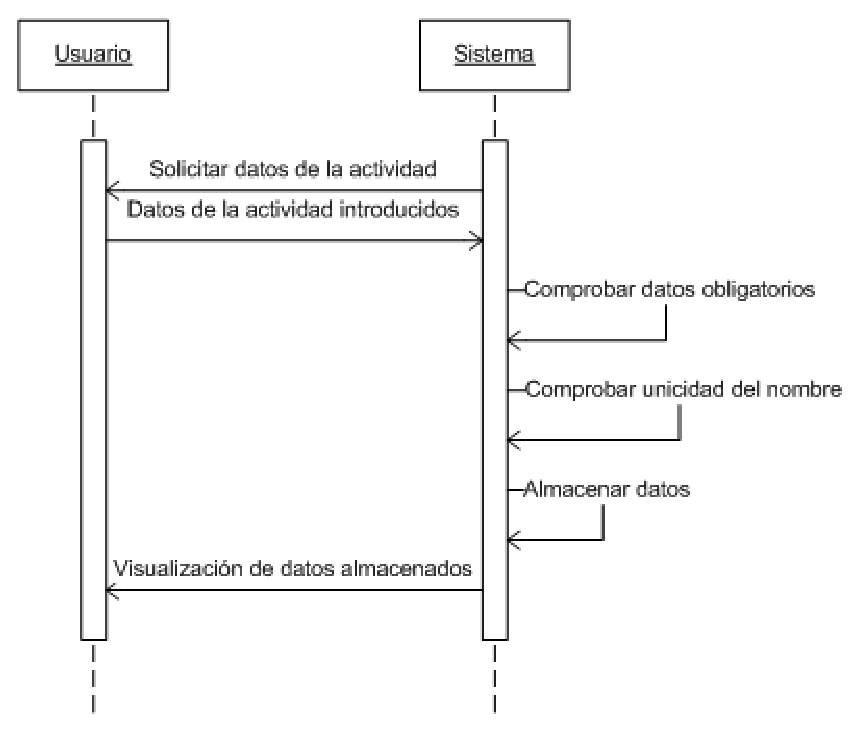
\epsfig{file=imagenes/secuencia/crear_actividad,width=4in}
\caption{Diagrama de secuencia: creación de actividad.}
\label{fig:crear_actividad}
\end{figure}

\begin{figure}
\centering
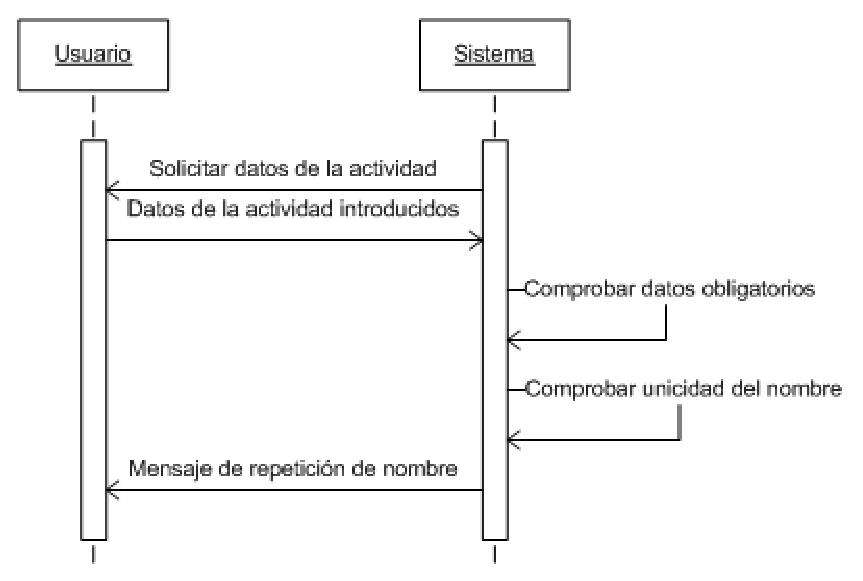
\epsfig{file=imagenes/secuencia/crear_actividad_repetida,width=4in}
\caption{Diagrama de secuencia: creación de actividad con repetición.}
\label{fig:crear_actividad_repetida}
\end{figure}

\begin{figure}
\centering
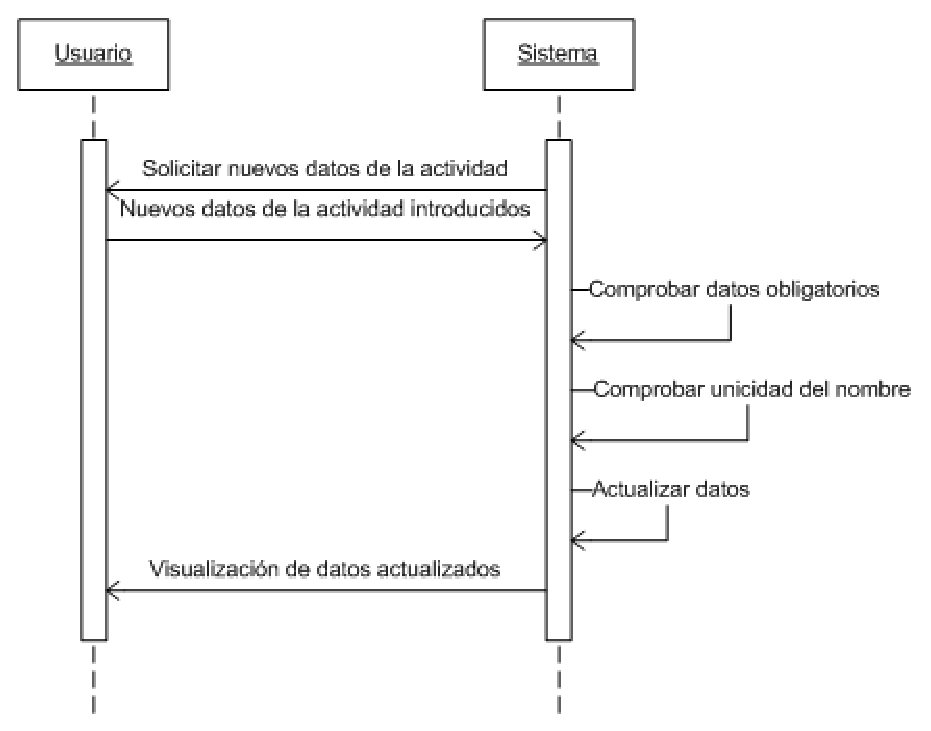
\epsfig{file=imagenes/secuencia/actualizar_actividad,width=4in}
\caption{Diagrama de secuencia: modificación de actividad.}
\label{fig:actualizar_actividad}
\end{figure}

\begin{figure}
\centering
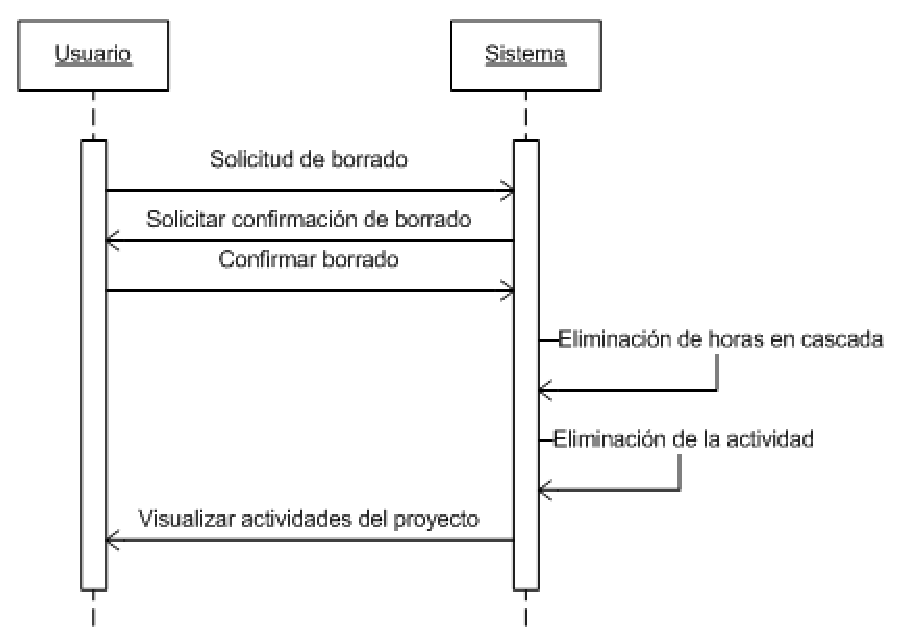
\epsfig{file=imagenes/secuencia/eliminacion_actividad,width=4in}
\caption{Diagrama de secuencia: eliminación de actividad.}
\label{fig:eliminacion_actividad}
\end{figure}

\begin{figure}
\centering
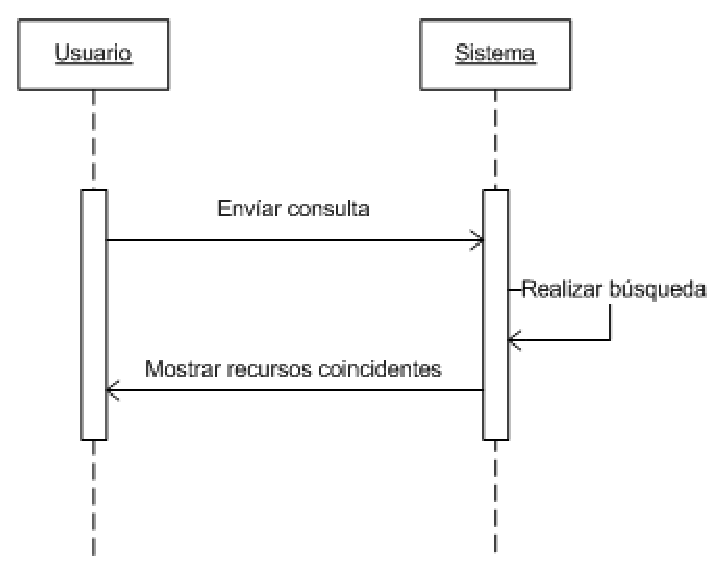
\epsfig{file=imagenes/secuencia/buscar_recurso,width=3.5in}
\caption{Diagrama de secuencia: búsqueda de recurso.}
\label{fig:buscar_recurso}
\end{figure}

\begin{figure}
\centering
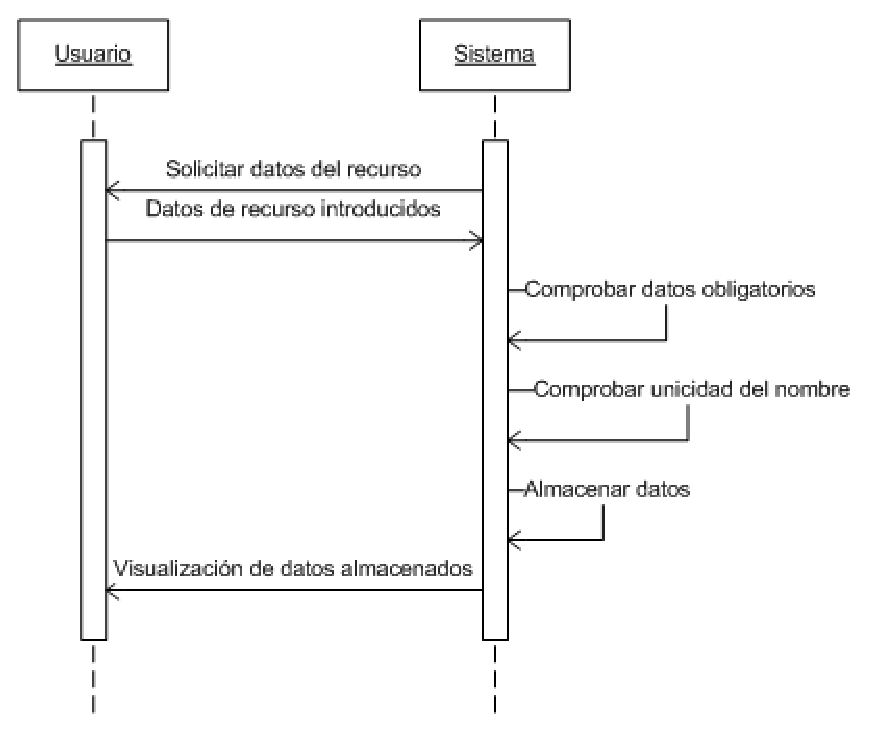
\epsfig{file=imagenes/secuencia/crear_recurso,width=4in}
\caption{Diagrama de secuencia: creación de recurso.}
\label{fig:crear_recurso}
\end{figure}

\begin{figure}
\centering
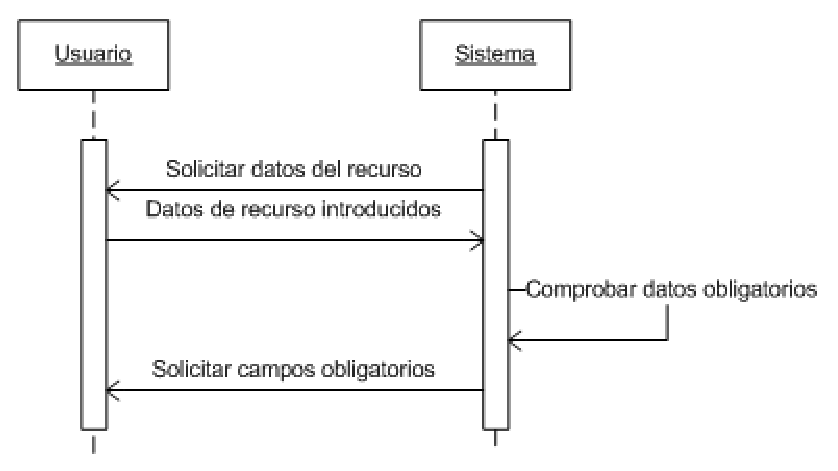
\epsfig{file=imagenes/secuencia/crear_recurso_campos,width=4in}
\caption{Diagrama de secuencia: creación de recurso incompleta.}
\label{fig:crear_recurso_campos}
\end{figure}

\begin{figure}
\centering
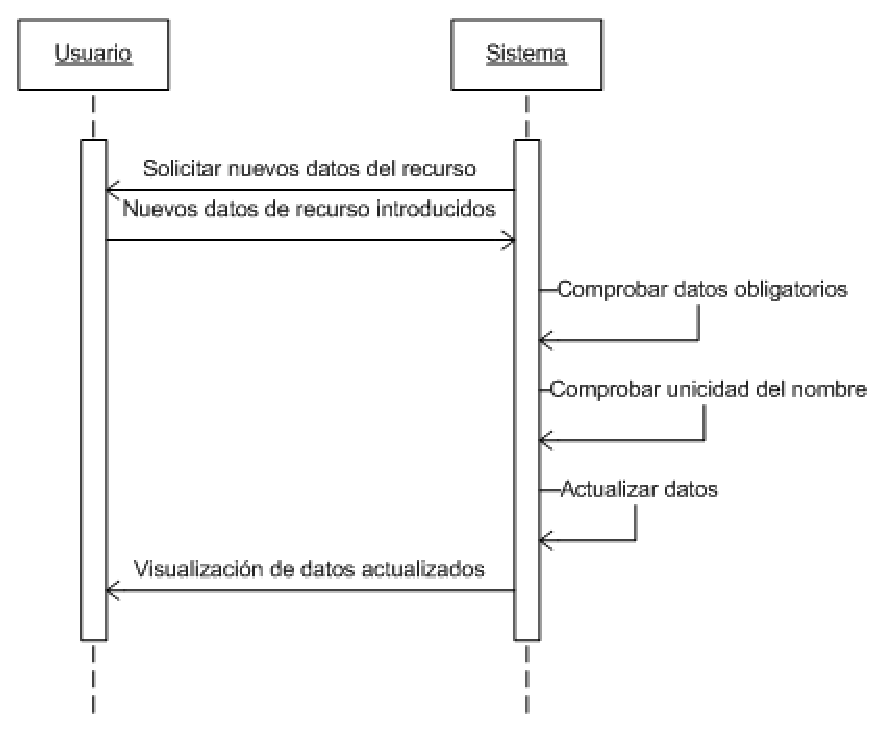
\epsfig{file=imagenes/secuencia/actualizar_recurso,width=4in}
\caption{Diagrama de secuencia: modificación de recurso.}
\label{fig:actualizar_recurso}
\end{figure}

\begin{figure}
\centering
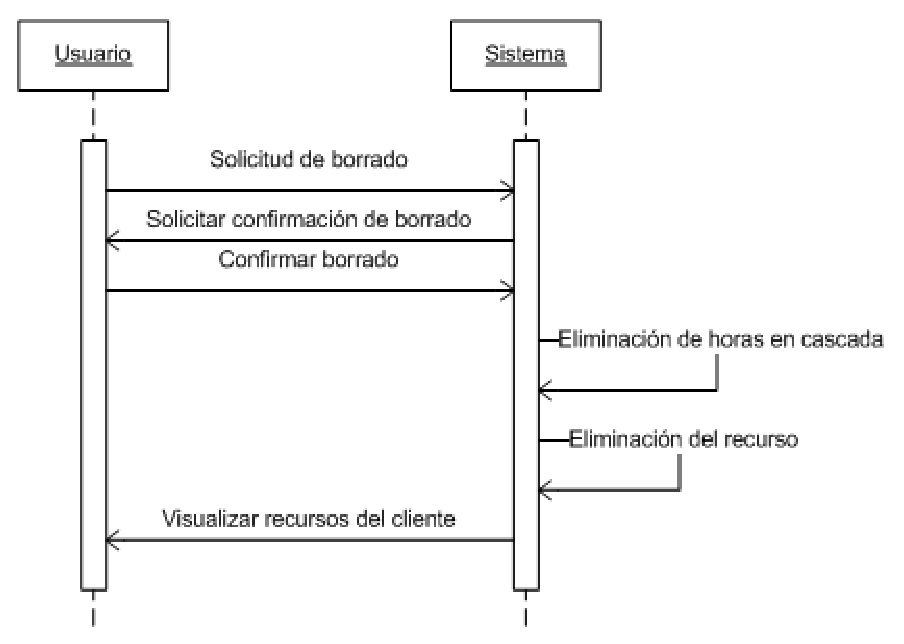
\epsfig{file=imagenes/secuencia/eliminacion_recurso,width=4in}
\caption{Diagrama de secuencia: eliminación de recurso.}
\label{fig:eliminacion_recurso}
\end{figure}

\begin{figure}
\centering
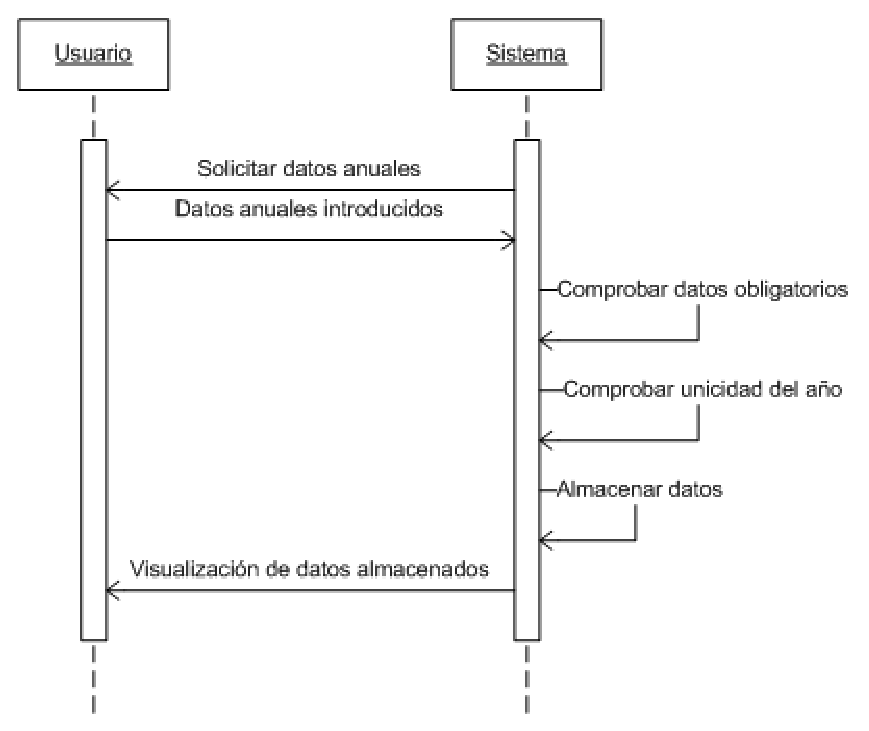
\epsfig{file=imagenes/secuencia/crear_registro_anual,width=4in}
\caption{Diagrama de secuencia: creación de registro anual.}
\label{fig:crear_registro_anual}
\end{figure}

\begin{figure}
\centering
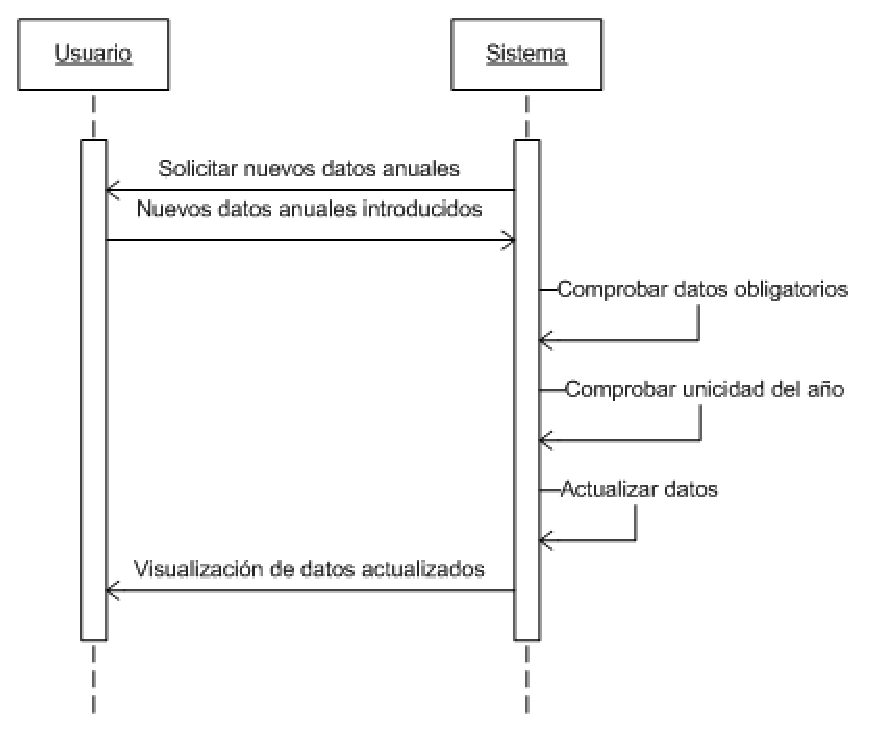
\epsfig{file=imagenes/secuencia/modificar_registro_anual,width=4in}
\caption{Diagrama de secuencia: modificación de registro anual.}
\label{fig:modificar_registro_anual}
\end{figure}

\begin{figure}
\centering
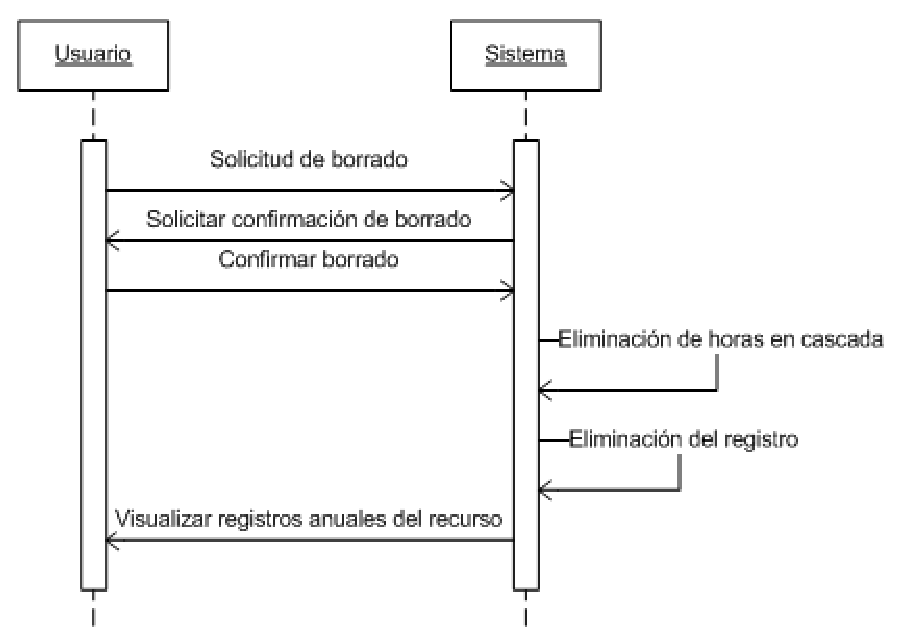
\epsfig{file=imagenes/secuencia/eliminacion_registro,width=4in}
\caption{Diagrama de secuencia: eliminación de registro anual.}
\label{fig:eliminacion_registro}
\end{figure}

\begin{figure}
\centering
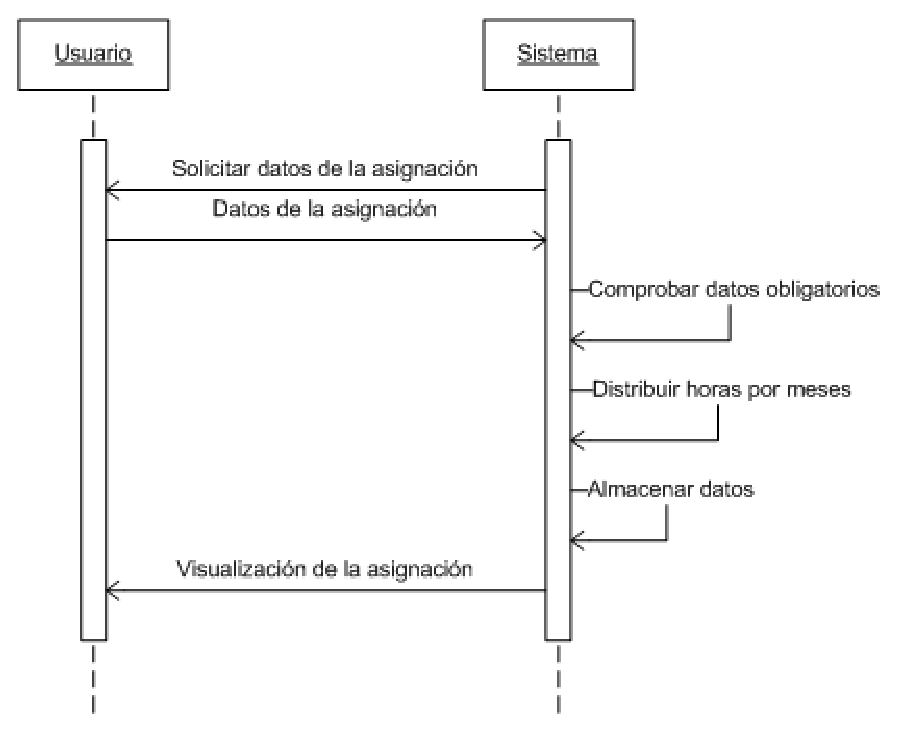
\epsfig{file=imagenes/secuencia/asignacion_horas,width=4in}
\caption{Diagrama de secuencia: asignación de horas.}
\label{fig:asignacion_horas}
\end{figure}

\begin{figure}
\centering
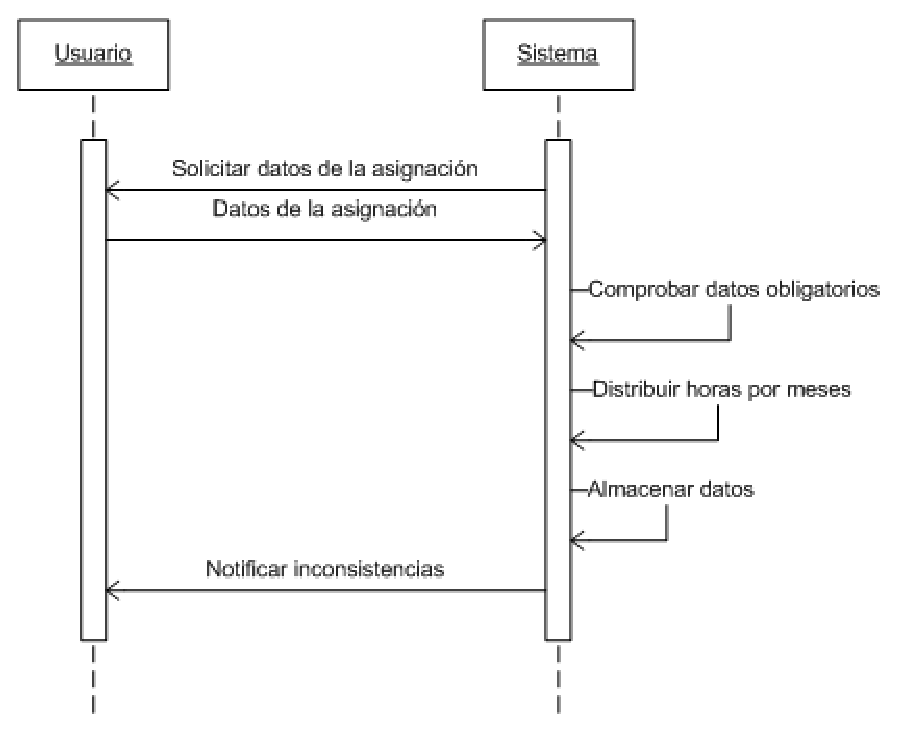
\epsfig{file=imagenes/secuencia/asignacion_horas_inconsistencia,width=4in}
\caption{Diagrama de secuencia: asignación de horas con inconsistencias.}
\label{fig:asignacion_horas_inconsistencia}
\end{figure}





\chapter{Implementación}
\label{chp:implementacion}
\thispagestyle{empty}
\noindent \textit{En este capítulo se describirán muy brevemente las
principales tecnologías usadas en el desarrollo, se darán algunos datos
acerca de las librerías empleadas y se explicarán con cierto nivel de detalle
los algoritmos más representativos.}
\section{Tecnologías}

\subsection{Lenguajes}

Como ya se ha hablado en varias ocasiones a lo largo de la memoria de los
lenguajes empleados, se remite al lector a las secciones \ref{sec:tecnologias}
y \ref{sec:diseno_del_sistema} para conocer las motivaciones de la elección de
PHP y el modo en que se ha empleado en el sistema.

A modo de introducción para el lector no iniciado (y con el deseo de que sean
unos pocos), \textbf{PHP} es un lenguaje de programación interpretado --en
contraste con los compilados-- especialmente útil para el desarrollo web del
lado del servidor, de manera que es muy usado en la programación de webs
dinámicas, delimitando el código PHP mediante los delimitadores
\verb|<?php| y \verb|?>|. Así, una primera aproximación sería:

\begin{lstlisting}
<!DOCTYPE html>
<html>
  <head>
    <meta charset="utf-8" />
    <title>Pruebe PHP</title>
  </head>
  <body>
  <?php
  echo 'Hola Mundo';
  /* echo("Hola Mundo"); tambien funciona,
  pero echo no es una funcion, sino un
  constructor del lenguaje. */
  ?>
  </body>
</html>
\end{lstlisting}

\textbf{JavaScript} también es un lenguaje de programación interpretado. Se
define como orientado a objetos, basado en prototipos, imperativo, débilmente
\textit{tipado} y dinámico. Uno de sus uso principales es el que se le ha dado
en este proyecto, para mejorar la experiencia del usuario al interactuar con la
interfaz. Como se explicará más adelante, también es crucial en la técnica de
desarrollo web Ajax, empleada en el buscador global. De nuevo, a modo de
simplísima introducción:

\begin{lstlisting}
<!DOCTYPE html>
<html>
  <head>
    <meta charset="utf-8" />
    <title>Pruebe JavaScript</title>
  </head>
  <body>
    <script type="text/javascript">
      document.write('Hola Mundo');
    </script>
    <noscript>
      <p>Su navegador no tiene soporta para JavaScript, 
      o este esta deshabilitado.</p>
    </noscript>
  </body>
</html>
\end{lstlisting}

A parte de PHP JavaScript, se ha hecho uso, por supuesto, de HTML, el lenguaje
de marcas predominante para la construcción de páginas web, así como de CSS
para la definición de los estilos del formato.

\subsection{Ajax}
\label{sec:fundamentos_ajax}

Ajax se utiliza para la creación de webs dinámicas y rápidas, permitiendo la
transferencia de información con el servidor de manera transparente para el
usuario, es decir, sin que este tenga que recargar la página. Su uso en la
actualidad está muy extendido en aplicaciones con alto grado de dinamicidad,
como Google Maps o Facebook.

Ajax está basado en estándares de Internet, y para su funcionamiento (figura
\ref{fig:ajax}) usa una combinación de:

\begin{itemize}
\item El objeto XMLHttpRequest

\item JavaScript/DOM (para mostrar/interactuar con la información)

\item CSS (para dar estilo a los datos)

\item XML (usado frecuentemente como el formato de transferencia de datos)
\end{itemize}

\begin{figure}
\centering
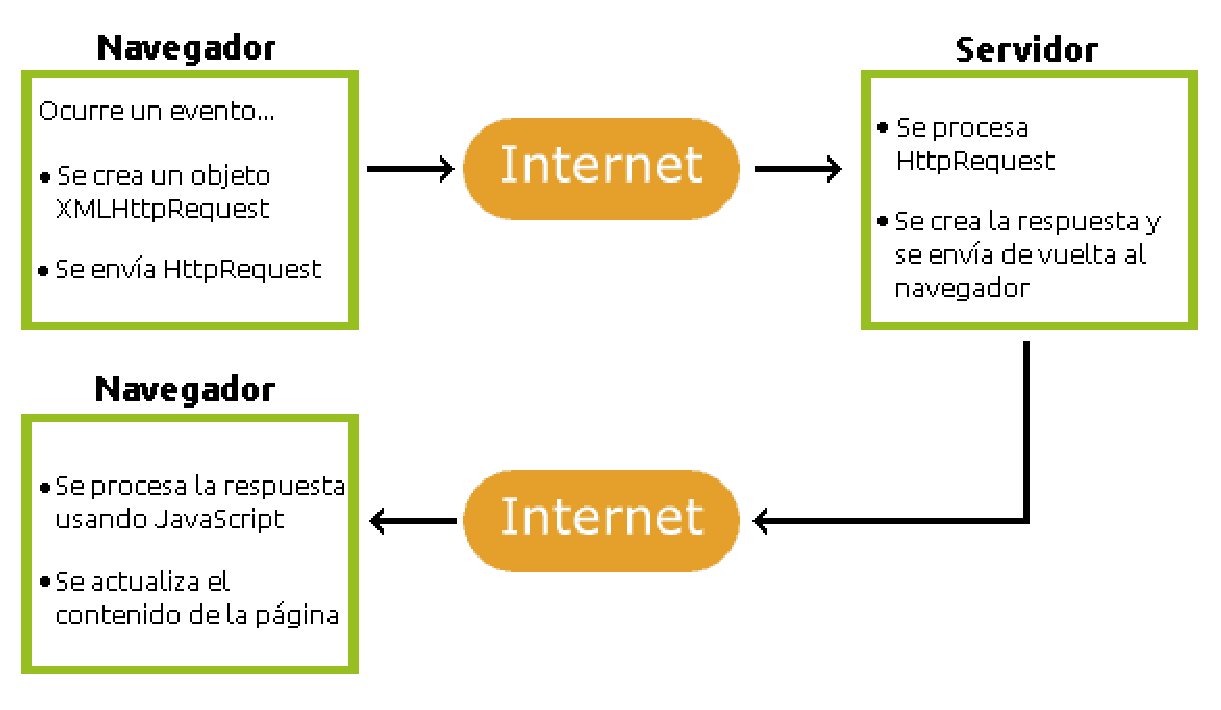
\epsfig{file=imagenes/ajax.eps,width=5.28in}
\caption{Funcionamiento de Ajax.}
\label{fig:ajax}
\end{figure}

Curiosamente, la primera aplicación Ajax que alcanzó la popularidad a nivel
mundial fue Google Suggest (las sugerencias del conocido buscador, lanzadas en
diciembre de 2004), y este ha sido precisamente uno de los usos que se le ha
dado en el marco de este proyecto: sugerir proyectos y clientes que listados de
otro modo resultarían demasiado pesados. La otra parte de la herramienta que
hace uso intensivo de Ajax es el buscador global.

Además, Ajax a pesar de ser una tecnología relativamente reciente, no solo es
compatible con los navegadores modernos, sino que también está soportado en IE5
e IE6, gracias a una implementación particular del objeto HttpRequest que estos
navegadores ya incluían.

\begin{lstlisting}
var xmlhttp;
if (window.XMLHttpRequest)
  {// codigo para IE7+, Firefox, Chrome, Opera, Safari
  xmlhttp=new XMLHttpRequest();
  }
else
  {// codigo para IE6, IE5
  xmlhttp=new ActiveXObject("Microsoft.XMLHTTP");
  }
\end{lstlisting}

\section{Librerías}

El uso de librerías forma parte del día a día del desarrollo web y de la
programación en general. En este caso se han usado dos librerías básicas y de
naturaleza muy distinta, una librería de JavaScript y otra PHP. Además, la
aplicación ya contaba con una librería para la selección de fechas en formato
calendario, pero debido a que ya estaba en uso y a su simplicidad, no se
describirá.

\subsection{Sorttable}

\textit{Sorttable}\footnote{Sitio oficial de la librería:
\href{http://www.kryogenix.org/code/browser/sorttable/}{
kryogenix.org/code/browser/sorttable/}} es una librería (o minilibrería)
JavaScript que permite la ordenación de filas de tablas una vez cargadas y sin
necesidad de recargar la página. El uso de esta librería no responde a una
necesidad específica, pero, de acuerdo con el cliente, la capacidad para ordenar
cualquier tabla según el tipo de dato que contengan es una de las cosas que más
se echan de menos en las aplicaciones web en contraste con las aplicaciones de
escritorio.

Una de las formas más comunes de resolver esta carencia es
recargando la página pasándole al servidor la información acerca de como desean
ordenarse los datos. Sin embargo, gracias al uso de JavaScript, podemos lograr
este mismo resultado sin recargar la página y sin consumir recursos del lado
del servidor siguiente unas pautas muy sencillas acerca del buen formato de la
tabla: es necesario usar bloques de cabecera, cuerpo y pie de tabla:
\verb|<thead>|, \verb|<tbody>| \verb|<tfoot>|).

La librería es capaz de ordenar automáticamente los tipos de datos más comunes,
pero si se necesitan ordenar tipos de fecha complejos o personalizados (fechas
en formatos especiales), también ofrece la opción de ordenar por criterios
transparentes al usuario y distintos a lo que se ve en la tabla. Así, por
ejemplo, si se desea que ordene los meses pero los estamos mostranto en formato
texto (enero-diciembre), simplemente tendríamos que pasarle la información en
formato 1-12 a través del atributo \verb|sorttable_customkey|.

Finalmente, el usuario solo tendrá que pinchar sobre la cabecera de la columna
para reordenar las filas.

Es importante resaltar que la librería tiene licencia X11 del
\textit{Massachusetts Institute of Technology }(MIT), que autoriza su uso sin
restricciones con la condición de incluir el (breve) texto de la
licencia\footnote{La licencia completa puede consultarse aquí:
\href{http://www.xfree86.org/3.3.6/COPYRIGHT2.html}{
xfree86.org/3.3.6/COPYRIGHT2.html}} allá donde sea usada.

\subsection{PHPExcel}

PHPExcel\footnote{Sitio oficial de la librería:
\href{http://www.phpexcel.net}{
phpexcel.net}} es una poderosa librería que
proporciona un conjunto de clases PHP que permiten la lectura y escritura de
documentos Excel (2010 y anteriores). Incluye opciones para el manejo de
metadatos, estilos, múltiples hojas de cálculo, congelación de paneles, cálculo
de fórmulas Excel... La imagen \ref{fig:ejemplo_PHPExcel} representa algunas de
las cosas que se pueden conseguir con el uso de esta librería.

Esta librería se ha usado para exportar informes complejos en relación a la
asignación de horas de los empleados. Como se indicó en la sección
\ref{sec:requisitos_informes} sobre los requisitos de los informes, se
determinó que era importante conservar la funcionalidad anterior --el registro
de la distribución de horas se realizaba en hojas de cálculo--, por lo que se
creó la opción de exportar un resumen de la participación de los empleados en
todos los proyectos de la empresa (veáse la figura
\ref{fig:resumen_horas_asignadas_proyectos} del Manual de Usuario).

\begin{figure}
\centering
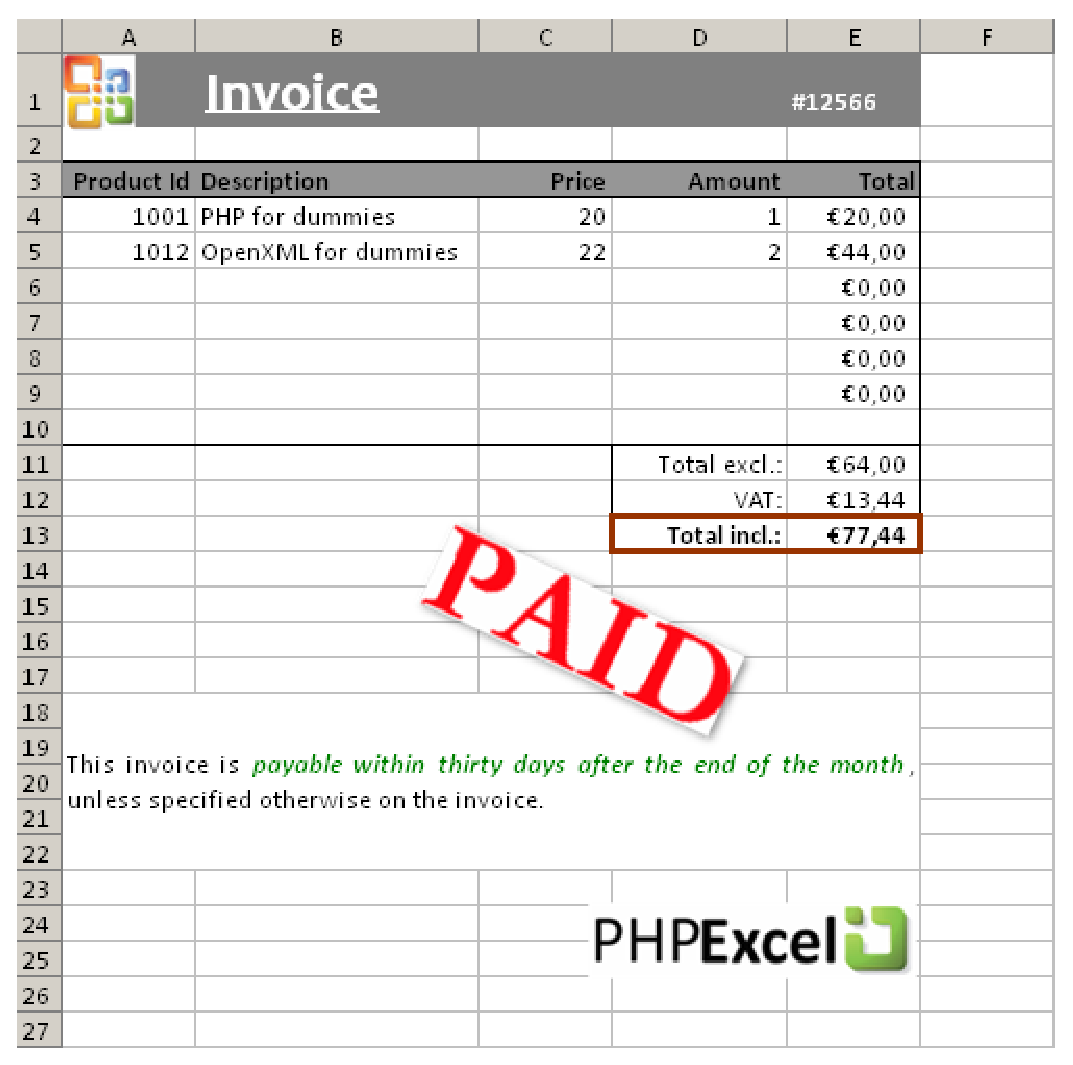
\epsfig{file=imagenes/ejemplo_PHPExcel.eps,width=3.5in}
\caption{Ejemplo de hoja de cálculo compleja.}
\label{fig:ejemplo_PHPExcel}
\end{figure}

El manejo de esta librería no es sencillo y requirió de un periodo de estudio
de aproximadamente una semana, pero el nivel de detalle de la documentación
facilitó enormemente esta tarea.

Por último, dejar constancia de que la librería tiene una licencia
LGPL\footnote{La licencia completa puede consultarse aquí:
\href{http://www.gnu.org/licenses/lgpl.html}{
gnu.org/licenses/lgpl.html}} (GNU
Lesser General Public License), que permite su uso libre pero no la
modificación del Software.

\subsection{JQuery}

La popularidad de JQuery\footnote{Sitio oficial de la librería:
\href{http://jquery.com/}{
jquery.com}} hizo que tanto el cliente como el
proyectante se interesasen por las posibilidades de esta librería de JavaScript,
por lo que fue estudiada con relativa profundidad. Finalmente, se decidió no
incluirla en el marco de este proyecto, pero el nuevo conocimiento adquirido
sería usado en otros desarrollos, como se explica más adelante en el capítulo
\ref{chp:conclusiones}.

\section{Detalles de la implementación. Algoritmos representativos}

\subsection{Distribución de horas por mes}
\label{sec:algoritmo_distribucion}

La asignación de horas debe seguir los requisitos funcionales descritos en la
sección \ref{sec:requisitos_gestion_horas}. Para facilitar la labor del lector,
se copia a continuación el punto que hace referencia a la distribución de las
horas:

\begin{quote}
La asignación de horas a un periodo se repartirá internamente por meses (no
días), de manera que las horas asignadas a un periodo que comprenda dos meses o
más se repartirán porcentualmente teniendo en cuenta el número de días
laborables de cada mes, y cuando sea posible, en múltiplos de 5. Debido a la
excesiva complejidad que se añadiría, no se tienen en cuenta las horas del
empleado en otros proyectos en el momento de la asignación.
\end{quote}

Secuencia de la distribución:
\begin{enumerate}
\item En primer lugar, debemos recoger los datos necesarios para realizar la
asignación, que llegan a partir del formulario de asignación (veáse la figura
\ref{fig:form_asig_horas} del Manual de Usuario). Estos datos son:

  \begin{itemize}
  \item Identificador del empleado.
  \item Identificador de la actividad.
  \item Tipo de horas (presentadas, aprobadas, justificadas).
  \item Fecha de inicio de la asignación.
  \item Fecha de fin de la asignación.
  \item Número de horas a distribuir.
  \item Descripción de la labor del empleado.
  \end{itemize}

\item Ahora se deben introducir los datos de la asignación en la tabla
PERSONAL\_ACTIVIDAD:

\begin{lstlisting}
INSERT INTO personal_actividad
(id_personal,id_actividad,f_ini,f_fin,descripcion)
VALUES
('$personal','$actividad','$f_ini_unix','$f_fin_unix','$descripcion')";
\end{lstlisting}

\item Se calculará el número de días laborables entre las dos fechas:

\begin{lstlisting}
function laborables($f_ini_unix,$f_fin_unix) {
	$current_date = $f_ini_unix; 
	$num = 0;
	while ($current_date <= $f_fin_unix) {
		$dia = date('w',$current_date);
		if ($dia > 0 && $dia < 6 &&
!esFestivoNacional(date('j',$current_date), date('n',$current_date))) {
			$num++;
		}
		$current_date += 86400;
	}
	return $num;
}
\end{lstlisting}

\textit{Nota: De hecho, esta función, que estuvo en funcionamiento durante meses
sin que el proyectante advirtiera ninguna anomalía, es incorrecta, como se
advertiría gracias a un plan de pruebas que se describirá en el capítulo
\ref{chp:pruebas}.}

\item A partir del número de días, se calculará la asignación de horas diaria
de forma proporcional, corrigiendo los excesos (se corrigen los excesos
provocados por la propia actividad, no en combinación con otras). Asimismo, se
calculará el número de meses completos (quitando los extremos) y de años
implicados en la asignación:

\begin{lstlisting}
$horas_dia = $duracion_en_horas / $duracion_en_dias;
if ($horas_dia > 8) {
	$horas_dia = 8;
}
$num_anios = $anio_fin - anio_inicio;
$num_meses_completos = ($num_anios * 12) + ($mes_fin - $mes_inicio) - 1;
\end{lstlisting}

Nótese que si solo hay un mes implicado en la asignación, el número de meses
completos se considerará, por convención, -1, y en este caso, se asignarán
todas las horas a ese mes, de nuevo, corrigiendo al máximo si hay exceso:

\begin{lstlisting}
if ($num_meses_completos == -1){
	$horas_aux = $duracion_en_horas;
	if($horas_aux > $duracion_en_dias * 8) {
		$horas_aux = $duracion_en_dias * 8;
	}
}
\end{lstlisting}

\item Si hay más de un mes implicado en la asignación, calculamos el número de
días laborables del primer mes desde la fecha de inicio hasta el final del mes,
y multiplicamos esos días por el número de horas que era necesario trabajar al
día según el número de días laborables global. Después, en el primer mes,
aumentamos el número de horas hasta el primer múltiplo de 5 siempre que el
valor de horas sea mayor que 5; si no, simplemente redondeamos al alza el número
de horas para el mes. Finalmente, comprobamos que no nos pasamos del máximo
posible ni de lo deseado y restamos el número de horas del mes al valor de horas
global para seguir con los meses siguientes.

\begin{lstlisting}
$laborables =
laborables($f_ini_unix,mktime(23,59,59,$mes_inicio+1,0,$anio_inicio));
$horas_aux = $horas_dia * $laborables;
if($horas_aux > 5) {
	$horas_aux = ceil($horas_aux / 5) * 5;
} else {
	$horas_aux = ceil($horas_aux);
}
if($laborables * 8 < $horas_aux)
	$horas_aux = $laborables * 8;
if($duracion_en_horas < $horas_aux)
	$horas_aux = $duracion_en_horas;
$duracion_en_horas -= $horas_aux;
\end{lstlisting}

\item Para los meses intermedios (lo que se llamó antes meses completos),
empleamos un bucle \verb|for| , ya que conocemos el mes inicial y el número de
meses completos. Así, calcularemos el número de días laborables del mes al que
se van a asignar las horas en cada caso y, como antes, se multiplicarán por la
asignación diaria prevista. Si dicha asignación es mayor que 5, se aumentarán
hasta el primer múltiplo de 5, y si no, solamente hasta el primer entero. Dado
que estamos redondeando al alza, haremos las comprobaciones pertinentes para no
pasarnos de la asignación global deseada ni de la asignación del mes máxima.
Finalmente, restaremos el valor obtenido al global a asignar:

\begin{lstlisting}
for ($mes_actual = $mes_inicio; $mes_actual < $mes_inicio +
$num_meses_completos; $mes_actual++) {
	$fecha_aux = mktime(0,0,0,$mes_actual + 1,1,$anio_inicio);
	$laborables = laborables($fecha_aux,mktime(0,0,0,$mes_actual +
2,0,$anio_inicio));
	$horas_aux = $horas_dia * $laborables;
	if($horas_aux > 5) {
		$horas_aux = ceil($horas_aux / 5) * 5;
	} else {
		$horas_aux = ceil($horas_aux);
	}
	if($laborables * 8 < $horas_aux)
		$horas_aux = $laborables * 8;
	if($duracion_en_horas < $horas_aux)
		$horas_aux = $duracion_en_horas;
	$duracion_en_horas -= $horas_aux;
}
\end{lstlisting}

\item Y para acabar todo el proceso, debemos introducir en el último mes todas
las horas que no hayan sido asignadas, asegurándonos que no son excesivas para
el mes (aunque sería extraño, ya que se han ido adelantando horas en los meses
intermedios).

\begin{lstlisting}
$laborables = laborables(mktime(0,0,0,$mes_fin,1,$anio_fin),$f_fin_unix);
$horas_aux = $duracion_en_horas;
if($laborables * 8 < $horas_aux)
	$horas_aux = $laborables * 8;
\end{lstlisting}

\end{enumerate}

\subsection{Horas ocupadas de un empleado en un mes}

Para llevar un control exhaustivo de la consistencia de los datos de cada
empleado, debemos ser capaces de calcular el número de horas que tiene asignadas
en un mes concreto (y por extensión, en años concretos). En general, una
información así requeriría una simple consulta a la base de datos, pero en el
momento en que se introduce el concepto de estado del proyecto, el proceso se
complica. Al igual que se hizo en la sección anterior, se reproduce a
continuación el punto de los requisitos funcionales que hace mención a este
cálculo:

\begin{quote}
Debe ser posible visualizar cuántas horas tiene asignadas un recurso en
cada uno de sus registro anuales, así como el total de horas libres (sin
asignar hasta el total de su convenio). El concepto de total de horas asignadas
se define como la suma de los siguientes valores:
 
\begin{enumerate}
\item En los proyectos en fase de presentación, las horas presentadas aunque
sean cero, siempre que no se hayan imputado horas aprobadas o justificadas. En
el último caso, se tomarán las de la fase más avanzada.

\item En los proyectos en fase de aprobación, las horas aprobadas aunque sean
cero, siempre que no se hayan comenzado a imputar horas justificadas.

\item En proyectos justificados o concluidos, las horas justificadas aunque
sean cero.
\end{enumerate}

Obviamente, un recurso puede tener horas asignadas en cada uno de los tres
tipos de estados.
\end{quote}

Para resolver el problema, se hará una consulta a la base de datos de forma que
se obtengan las horas asignadas al empleado desglosadas por meses y actividades:
\begin{lstlisting}
SELECT estado,
	horas,
	horas_aprobadas,
	horas_justificadas
FROM personal_horas ph join actividad ac on 
	ph.id_actividad=ac.id join proyectos pr on 
	ac.proyecto=pr.id
WHERE ph.id_personal=$id_personal and 
	ph.anio=$anio and 
	ph.mes=$mes
\end{lstlisting}

No se pueden agrupar las horas por proyectos ni por estado de esos
proyectos porque puede haber meses sueltos en los que a pesar de que el estado
del proyecto sea presentado, el empleado tenga horas aprobadas o justificadas, y
de acuerdo a los requisitos, esas son las que deben contarse para llevar una
cuenta más real. Entonces, para cada fila devuelta, se comprobará que horas hay
que escoger:

\begin{lstlisting}
$horas_ocupadas = 0;
for ($i = 0; $i < $numero_de_filas; $i++) {
	if ($filas[$i]['horas_justificadas'] != 0 ||
		$filas[$i]['estado'] == "JUSTIFICADO" ||
		$filas[$i]['estado'] == "CONCLUIDO")
	{
		$horas_ocupadas += $filas[$i]['horas_justificadas'];
	}
	elseif ($filas[$i]['horas_aprobadas'] != 0 || 
		$filas[$i]['estado'] == "APROBADO")
	{
		$horas_ocupadas += $filas[$i]['horas_aprobadas'];
	}
	else {
		$horas_ocupadas += $filas[$i]['horas'];
	}
}
\end{lstlisting}

\subsection{Buscador}

En esta sección se revisarán los fundamentos del uso de Ajax para conseguir el
efecto de búsqueda instantánea. Una vez activo el cuadro de texto del buscador,
se usa el evento \verb|onkeyup| para llamar, cada vez que se presione una tecla,
a una función de JavaScript \verb|mostrarResultados(...)|,

\begin{lstlisting}
function mostrarResultados(elt,ini) {
	var q = elt.value;
	showHint(q,"searchResults","buscador",ini);
	document.getElementById("buscando").src=
		"imagenes/loading.gif";
	document.getElementById('searchResults').style.opacity=
		'0.6';
	document.getElementById('searchResults').style.filter=
		'alpha(opacity=60)';
	if(q != "")
		document.getElementById("searchResults").style.display=
			"block";
	else
		document.getElementById("searchResults").style.display=
			"none";
}
\end{lstlisting}

que hace visible el contenedor de los resultados y disminuye su opacidad,
incluye una imágen que informa que el buscador está cargando y llama a su vez a
la función \verb|showHint(...)|:

\begin{lstlisting}
function showHint(str,elt,lista,ini) {
	if (str.length==0) {
	  document.getElementById(elt).innerHTML="";
	  return;
	}
	xmlhttp=GetXmlHttpObject();
	if (xmlhttp==null) {
	  alert ("Su navegador no soporta XMLHTTP!");
	  return;
	}
	var url="include/"+lista+".php";
	url=url+"?q="+str.trim();
	url=url+"&ini="+ini;
	url=url+"&sid="+Math.random();
	xmlhttp.onreadystatechange=stateChanged;
	xmlhttp.open("GET",url,true);
	xmlhttp.send(null);
}
\end{lstlisting}

\verb|showHint| crea un objeto HttpRequest como se indicó en la sección
\ref{sec:fundamentos_ajax}, donde se introdujo brevemente la tecnología. Ese
objeto se guarda en la variable \verb|xmlhttp|, que no se ha creado en esta
función sino que es una variable global. También en esta función se crea la
consulta con método \verb|GET| que se envía al archivo \verb|buscador.php| para
que este mande los resultados de la búsqueda de vuelta a JavaScript.

Esa respuesta es manejada por la función \verb|stateChanged|, que también
revierte los aspectos visuales a opacidad total, quita la imagen que indica que
el buscador está cargando... y lo hace de la siguiente manera:

\begin{lstlisting}
function stateChanged() {
	if (xmlhttp.readyState==4) {
	document.getElementById("searchResults").innerHTML=
		xmlhttp.responseText;
	document.getElementById("buscando").src="imagenes/not_loading.png";
	setTimeout("document.getElementById(
		 'searchResults').style.opacity='1'",0);
	document.getElementById('searchResults').style.filter=
		'alpha(opacity=100)';
	if(ir_arriba==1)
		window.scrollTo(currentXPosition(),0);
	else
		ir_arriba=1;
	}
}
\end{lstlisting}

\begin{quote}
\textit{Nota: para detalles específicos sobre la implementación de la
funcionalidad completa del buscador --paginación, búsqueda selectiva, número de
resultados por página y navegación por teclado--, se remite directamente al
código.}
\end{quote}

\subsection{Sobre la implementación de la base de datos}

La base de datos ha sido implementada usando la interfaz gráfica del
cliente MySQL-Front, que se reseñará brevemente en el apéndice
\ref{apx:software_utilizado}. Dado que el motor de almacenamiento empleado en el
resto de la base de datos era MyISAM, se siguó con la misma metodología, si
bien podría haberse combinado con otros motores como InnoDB. Hay
que tener en cuenta que al crear una tabla, MyISAM acepta (no da
error) la sintaxis de claves foráneas pero no las implementa\footnote{Como se
puede leer en la documentación oficial: \newline
\href{http://dev.mysql.com/doc/refman/5.1/en/ansi-diff-foreign-keys.html }{
dev.mysql.com/doc/refman/5.1/en/ansi-diff-foreign-keys.html}}.

Así, no se han aprovechado las ventajas de la cláusula \verb|ON DELETE| en
combinación con \verb|CASCADE| y se han tenido que implementar este tipo de
comprobaciones en los \textit{scripts} PHP. Por ejemplo, al borrar una
actividad, es necesario explicitar el borrado de toda la información que hace
referencia a esa actividad para no dejar la base de datos en un estado
inconsistente.









\chapter{Pruebas}
\label{chp:pruebas}
\thispagestyle{empty}
\noindent \textit{En este capítulo se explicará cuál ha sido la metodología de
las pruebas y se detallará un test del algoritmo más representativo, el de la
distribución mensual de horas.}
Se ha hecho notar en anteriores capítulos que a pesar de no realizarse un
plan de pruebas exhaustivo y perfectamente documentado para cada parte del
desarrollo, la estrecha colaboración con el cliente ha hecho posible probar cada
evolución del código en un entorno prácticamente real.

Por supuesto, antes de informar al cliente de cualquier progreso en el
desarrollo, el proyectante realizaba pruebas básicas: desde que la interfaz
gráfica era perfectamente visible en los principales navegadores (Internet
Explorer 7+, Mozilla Firefox y Google Chrome, el empleado de forma preferida en
la empresa), hasta que los datos se guardaban y recuperaban correctamente de la
base de datos, pasando por la correcta solicitud de datos obligatorios y buen
comportamiento con datos de entrada inesperados.

De este manera, el módulo de personal fue probado por los empleados de
Ingeniería e Innovación a modo de registro de empleados --todavía no podían
asignarse horas ni guardar datos sobre actividades--, desde mediados de
agosto hasta diciembre del 2010. Aunque la funcionalidad era todavía muy básica,
el registro de los datos anuales de los empleados resultó útil por la
centralización de este tipo de información.

Similarmente, antes de que fuera posible conectar las actividades con los
empleados, se introdujeron datos de las actividades (planes de trabajo) de
proyectos concluidos a modo de testeo general, hecho del que se encargó
principalmente el proyectante durante su periodo de prácticas en la empresa.

Finalmente, una vez integrado todo el sistema, este empezó a utilizarse de
modo casi inmediato, ya que hubo que comenzar a justificar los primeros
proyectos con la nueva metodología requerida por la ADER, que se
describió con cierto detalle en la sección  \ref{sec:necesidad} al discutir la
necesidad del proyecto.

Apenas un mes después de que la herramienta comenzase a utilizarse en casos
reales y actuales y se hubieran reunido algunas sugerencias de modificación,
el proyectante sufrió una indisponibilidad familiar entre enero y febrero de
2011, periodo durante el cual cesó cualquier actividad del proyectante en
relación con la herramienta. Sin embargo, Ingeniería e Innovación siguió
utilizando el sistema sin mayores problemas.

\textit{Sin mayores problemas} no quiere decir \textit{sin problemas}, y hubo
uno en particular que, sin ser especialmente molesto, resultó de gran interés
para el proyectante hasta el punto de realizar la prueba que se detalla en la
siguiente sección.

\section{Prueba de distribución de horas y \textit{bug} horario}

El problema observado es que al pedirle a la herramienta que distribuyera un
número de horas en un espacio de tiempo, había ocasiones ($\sim 5\%$, como se
comprobará) en que no se distribuían todas las horas, tal y como uno esperaría.
Había una diferencia entre lo que se pedía distribuir y el resultado de la
distribución.

Se ha comentado anteriormente que la aplicación corrige los excesos a nivel del
proyecto: si se intenta asignar 300 horas a un empleado en un mismo proyecto en
un mes, esa cifra se va a reducir al número de días laborables del mes
multiplicadas por ocho. No es esa la fuente del error, pues es trivial, sino
que este se observó incluso cuando, en teoría, debería haber sido posible una
asignación total.

Dado que el algoritmo de distribución de horas (véase la sección
\ref{sec:algoritmo_distribucion} para recuperar los detalles) redondea al alza a
múltiplos de 5 cuando es posible, tiene en cuenta el número de días laborables
del mes..., resultaba difícil encontrar un error evidente en el código y
también datos de entrada que dieran error, por
lo que se escribió el \textit{script} del Apéndice
\ref{apx:script_distribucion}.

Los datos para el test son generados automáticamente, y se han
considerado suficientemente aleatorios dada la repetición periódica de los
calendarios (hay 14 distintos: el año puede comenzar en cualquiera de los 7 días
de la semana, y puede ser bisiesto o no):

\begin{lstlisting}
$mes_inicio = rand(1,12);
$anio_inicio = rand(2010,2025);
$dia_inicio = rand(1,date('t',mktime(0,0,0,$mes_inicio,1,$anio_inicio)));
$fecha_inicio = mktime(0,0,0,$mes_inicio,$dia_inicio,$anio_inicio);
$fecha_fin = mktime(0,0,0,$mes_inicio,$dia_inicio + rand(0,800),$anio_inicio);
$duracion_en_dias = laborables($fecha_inicio,$fecha_fin);
$duracion_en_horas = $duracion_en_dias * rand(1,900) / 100;
\end{lstlisting}

En el cuadro \ref{cua:resultados_script} se
muestran los resultados tras ejecutar el script original 10 veces.

\begin{table}
\centering
\footnotesize
\begin{tabular}{|c|c|c|c|}\hline
\textbf{Prueba} $\bf{n}$ & \textbf{Iteraciones} & \textbf{Errores} &
\textbf{\% Errores} \\\hline\hline
1 &  50 &   0 & 0\% \\\hline
2 &  50 &   4 & 8\% \\\hline
3 &  50 &   1 & 2\% \\\hline
4 &  50 &   3 & 6\% \\\hline
5 &  50 &   1 & 2\% \\\hline
6 &  50 &   4 & 8\% \\\hline
7 &  50 &   1 & 2\% \\\hline
8 &  50 &   5 & 10\% \\\hline
9 &  50 &   3 & 6\% \\\hline
10 &  50 &   3 & 6\% \\\hline
11 &  50 &   5 & 10\% \\\hline
12 &  50 &   2 & 4\% \\\hline
13 &  50 &   0 & 0\% \\\hline
14 &  50 &   4 & 8\% \\\hline
15 &  50 &   2 & 4\% \\\hline
16 &  50 &   2 & 4\% \\\hline
17 &  50 &   4 & 8\% \\\hline
18 &  50 &   1 & 2\% \\\hline
19 &  50 &   0 & 0\% \\\hline
20 &  50 &   3 & 6\% \\\hline
21 &  50 &   2 & 4\% \\\hline
22 &  50 &   1 & 2\% \\\hline
23 &  50 &   0 & 0\% \\\hline
24 &  50 &   2 & 4\% \\\hline
25 &  50 &   3 & 6\% \\\hline
26 &  50 &   2 & 4\% \\\hline
27 &  50 &   1 & 2\% \\\hline
28 &  50 &   2 & 4\% \\\hline
29 &  50 &   2 & 4\% \\\hline
30 &  50 &   4 & 8\% \\\hline\hline
\textbf{Total} &  \textbf{1500} &  \textbf{67} & \textbf{4.467\%} \\\hline
\end{tabular}
\caption{Prueba del algoritmo original.}
\label{cua:resultados_script}
\end{table}

A continuación, un resultado generado aleatoriamente que daba error:

\begin{itemize}
\item Fecha de inicio: 15/02/2011
\item Fecha de fin: 11/04/2012
\item Horas límite: 2368
\item Duración en horas: 2368
\item Horas por día: 8
\item Horas asignadas: 2360 
\item ¿Éxito?: No!
\item Diferencia: -8
\end{itemize}

Tras probar estos valores con una asignación en la herramienta, se vio que los
problemas venían siempre en los meses de marzo y octubre. «¡Eureka! El problema
es el cambio de hora». Al comprobar día a día si era laborable o no, la función
que se describió en la sección \ref{sec:algoritmo_distribucion} pasaba al día
siguiente de la siguiente forma:

\begin{lstlisting}
$current_date += 86400; //24*60*60=86400
\end{lstlisting}

Sin embargo, los días del cambio de hora NO tienen 24 horas, y PHP lo sabe, de
manera que se creaban errores cuando la exigencia de horas era máxima
(dedicación del empleado a jornada completa). La solución, pasar al día
siguiente de la siguiente manera:

\begin{lstlisting}
$current_date = 
	mktime(0,0,0,
		date('m',$current_date),
		date('d',$current_date)+1,
		date('Y',$current_date)
	);
\end{lstlisting}

Contribuía de manera vital al error que tanto las fechas de inicio como de fin
se pasaban en formato dd/mm/aaaa 00:00. Si se hubiera usado la notación
dd/mm/aaaa 23:59 para la fecha de fin, tampoco hubiese surgido el problema.

El proyectante ha ejecutado el \textit{script} modificado y una vez superadas
las 2000 pruebas no se había encontrado ningún error, es decir, siempre se han
guardado tantas horas como se había requerido, después de corregir a los
límites máximos mensuales.





\chapter{Consideraciones y conclusiones}
\label{chp:conclusiones}
\thispagestyle{empty}
\noindent \textit{En este último capítulo se hará un repaso a los
conocimientos adquiridos, el futuro del proyecto y del proyectante y se darán
algunos datos relativos al uso de la herramienta hasta la fecha actual.}
El proyecto en cuestión en la presente memoria ha sido el primero al que el
proyectante se ha enfrentado sin ningún tipo de supervisión técnica y fuera del
ámbito académico, lo que ha supuesto, en algunos momentos, un gran reto en los
planos personal y profesional, pero también la enorme satisfacción de
haber sido capaz de resolver, de mejor o peor manera, los obstáculos del camino.

\section{Conocimientos adquiridos}

Si bien uno de los objetivos del Proyecto Fin de Carrera es hacer uso de los
conocimientos adquiridos durante los cursos académicos, cabe destacar que, de la
ejecución del proyecto, el proyectante ha adquirido conocimientos muy valiosos
tanto a nivel técnico como de gestión.

En particular, el desconocimiento sobre PHP era casi absoluto; durante su etapa
de formación, el proyectante no había visto ni una línea de código en este
lenguaje, aunque sí se había comentado someramente. Sin el apoyo de un
formador experimentado, es muy probable que no se manejen de manera adecuada
algunos aspectos básicos del lenguaje, pero el aprendizaje autodidacta ha sido
satisfactorio y será sin duda completado en el futuro.

Otros conocimientos adquiridos o ampliados a nivel técnico incluyen una mayor
comprensión de la tecnología Ajax, HTML DOM, librerías como PHPExcel y el
framework JQuery, programas de creación de diagramas y, por supuesto, el
sistema de generación de documentos \LaTeX.

A nivel de gestión, el proyectante está seguro de que muchos de los errores de
este proyecto en cuanto a una correcta y completa planificación del trabajo a
realizar no se verán replicados en próximos proyectos.

\section{Algunos datos interesantes}

Se presentan a continuación algunas cifras extraídas de la base de datos que dan
una idea del uso real que se le está dando a la herramienta desde que pasó a ser
plenamente funcional en el último trimestre de 2010 hasta la fecha actual,
\today:

\begin{itemize}
\item Hay 550 registros anuales de \textbf{210 empleados} y
\item \textbf{118 actividades} en 41 proyectos
\item pertenecientes a 22 clientes,
\item sumando un total de \textbf{233111 horas presentadas y 178629
justificadas}.
\end{itemize}


\section{Futuro del proyecto}

En un principio, la previsible desvinculación del proyectante suponía la
completa paralización del desarrollo, pero, finalmente, las labores realizadas
a lo largo de las prácticas de empresa, que fueron más allá de la ejecución del
proyecto, le han valido un puesto en la plantilla.

Este hecho abre la posibilidad de mejorar la usabilidad del sistema por medio
de la automatización de algunos procesos, como la creación de nuevos registros
anuales, que ahora es manual. Otro campo de mejora es la visualización de los
datos, que ahora no es gráfica: en este sentido, podrían visualizarse las horas
en formato de cronograma o resumir algunos datos de forma estadística haciendo
uso de gráficas de barras, por ejemplo.

Sin embargo, las labores principales del proyectante en la empresa se
circunscriben más a la Gestión de Proyectos TIC.

\section{Labores del proyectante en otras partes de la aplicación}

Ya se ha comentado, tanto en la introducción como al tratar el diseño de la
interfaz, que la participación del proyectante en la ampliación de la
funcionalidad de la herramienta global no se ha ceñido exclusivamente a lo
discutido en esta memoria. Esas labores no se han incluido porque son de
naturaleza diversa y su tratamiento habría supuesto un alcance demasiado
extenso, pero han sido posibles gracias a los conocimientos adquiridos durante
la ejecución de este proyecto.

Dichas labores incluyen:

\begin{itemize}
\item Un completo gestor del tiempo que amplía notablemente las capacidades
anteriores de la aplicación, con vista de calendario y agenda, además de
estadísticas de uso de los empleados.
\item Un sistema simple de sugerencias, con prioridades y estados.
\item Un sistema de gestión documental simple y personalizado a las necesidades
de la empresa.
\item Informes gráficos de facturación comparada entre dos años, etc.
\end{itemize}

\begin{figure}
\centering
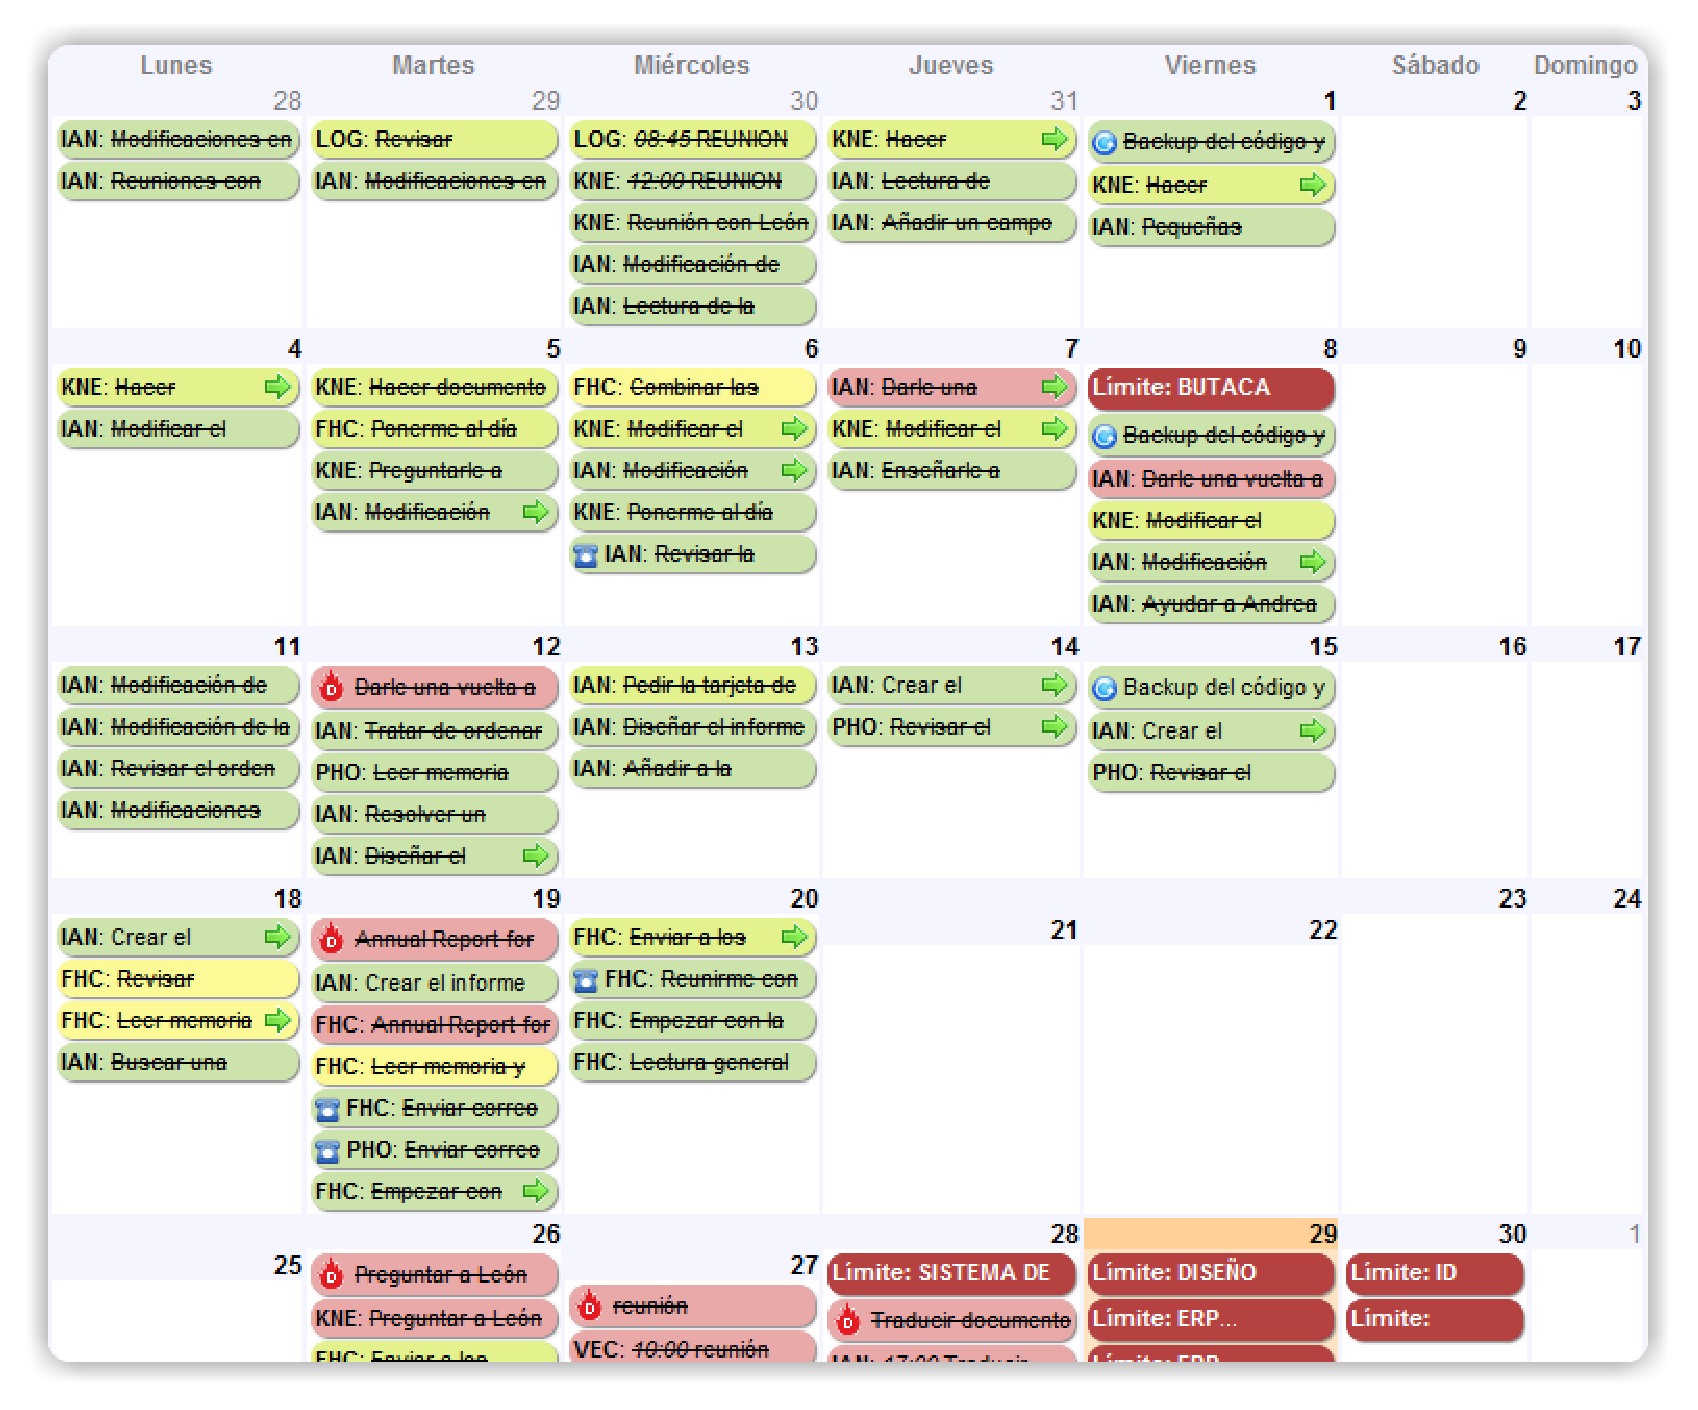
\epsfig{file=imagenes/otrosproyectos/tareas_cal2,height=5in,angle=90}
\caption{Vista de calendario del gestor del tiempo.}
\label{fig:tareas_cal2}
\end{figure}

\begin{figure}
\centering
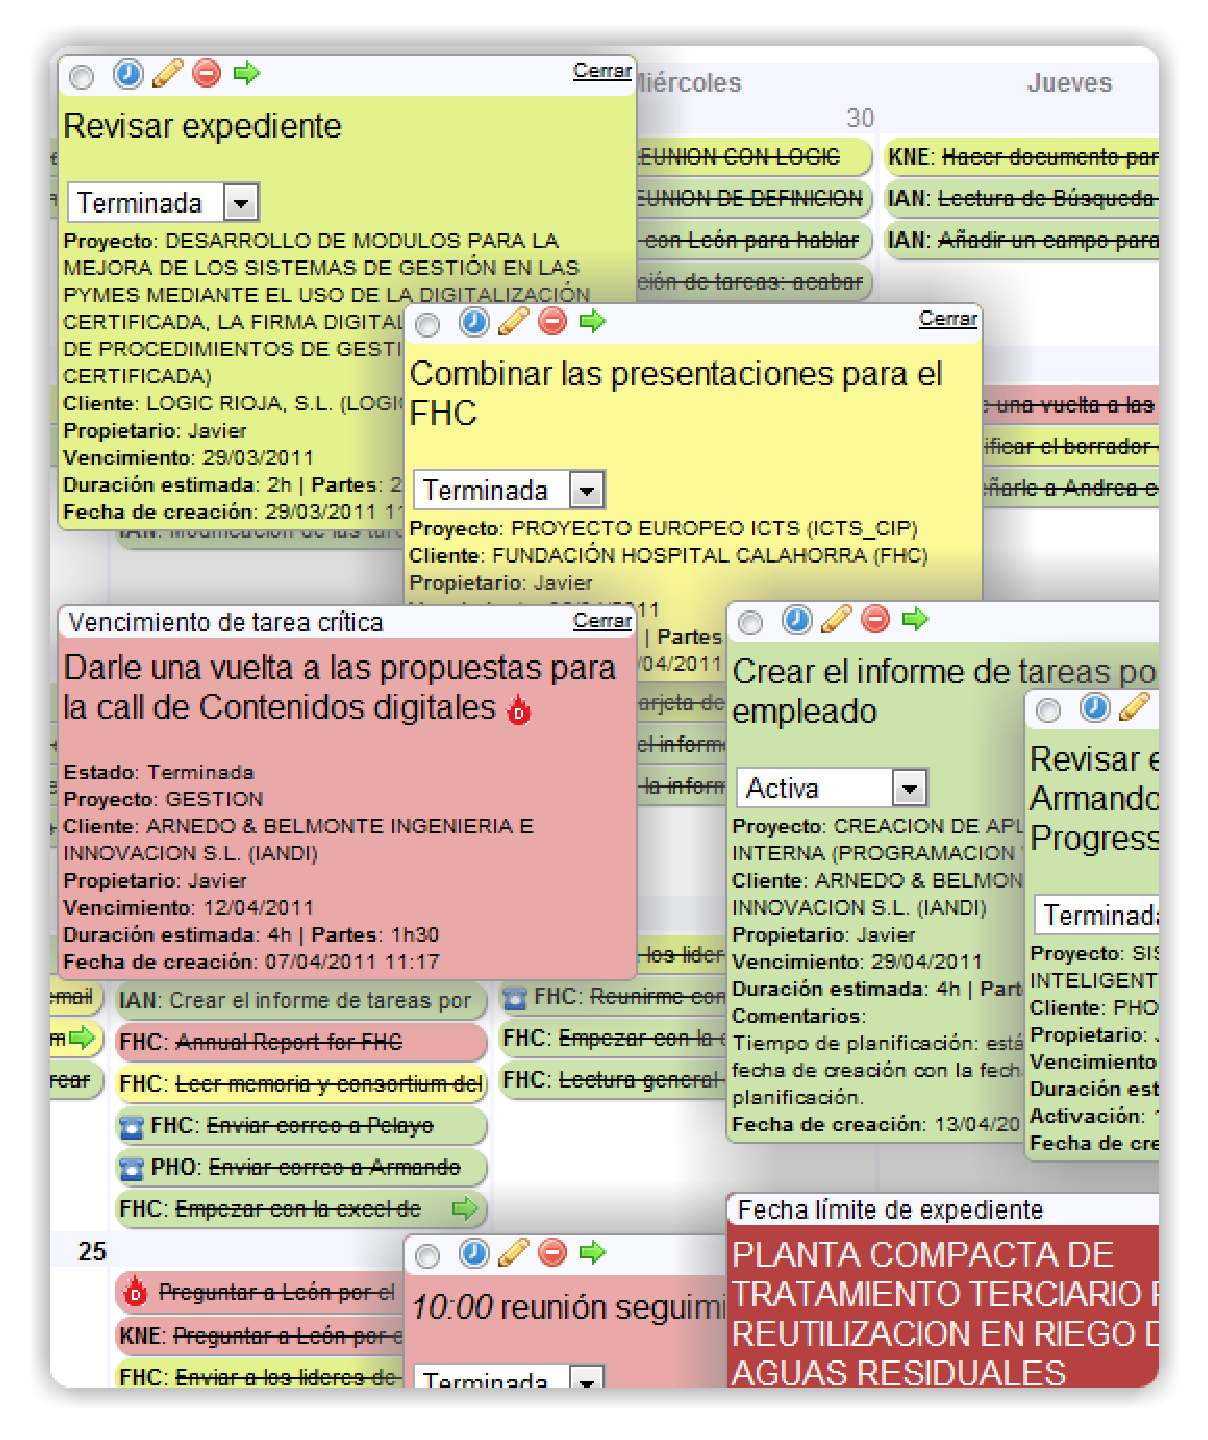
\epsfig{file=imagenes/otrosproyectos/tareas2,width=5in}
\caption{Detalle de las tareas del calendario.}
\label{fig:tareas2}
\end{figure}

\begin{figure}
\centering
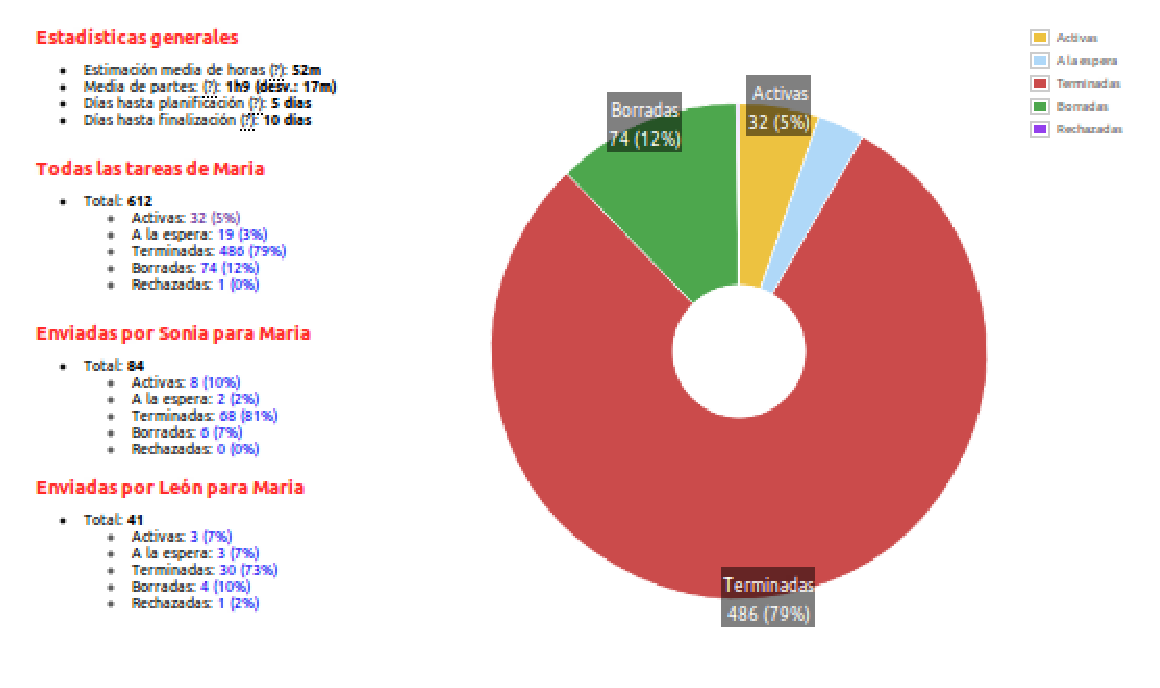
\epsfig{file=imagenes/otrosproyectos/tareas_stats,width=5in}
\caption{Estadísticas de tareas.}
\label{fig:tareas_stats}
\end{figure}

\begin{figure}
\centering
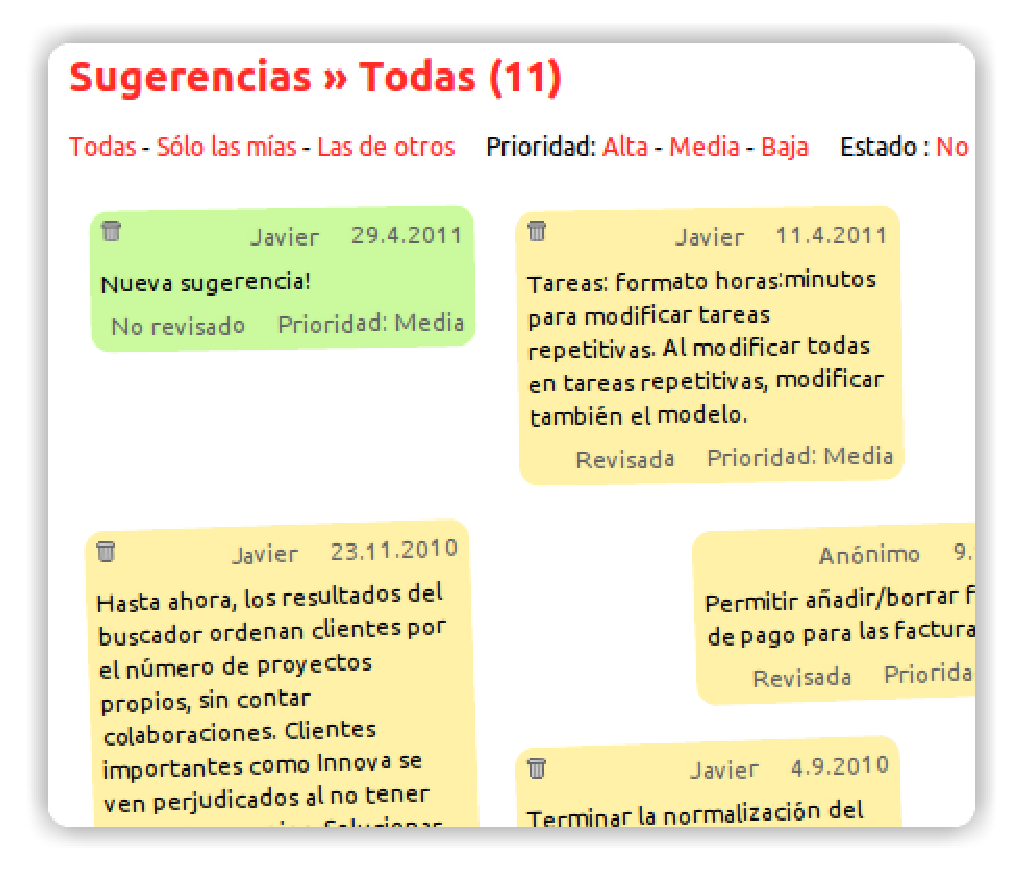
\epsfig{file=imagenes/otrosproyectos/sugerencias,width=4in}
\caption{Sistema de sugerencias.}
\label{fig:sugerencias}
\end{figure}

\begin{figure}
\centering
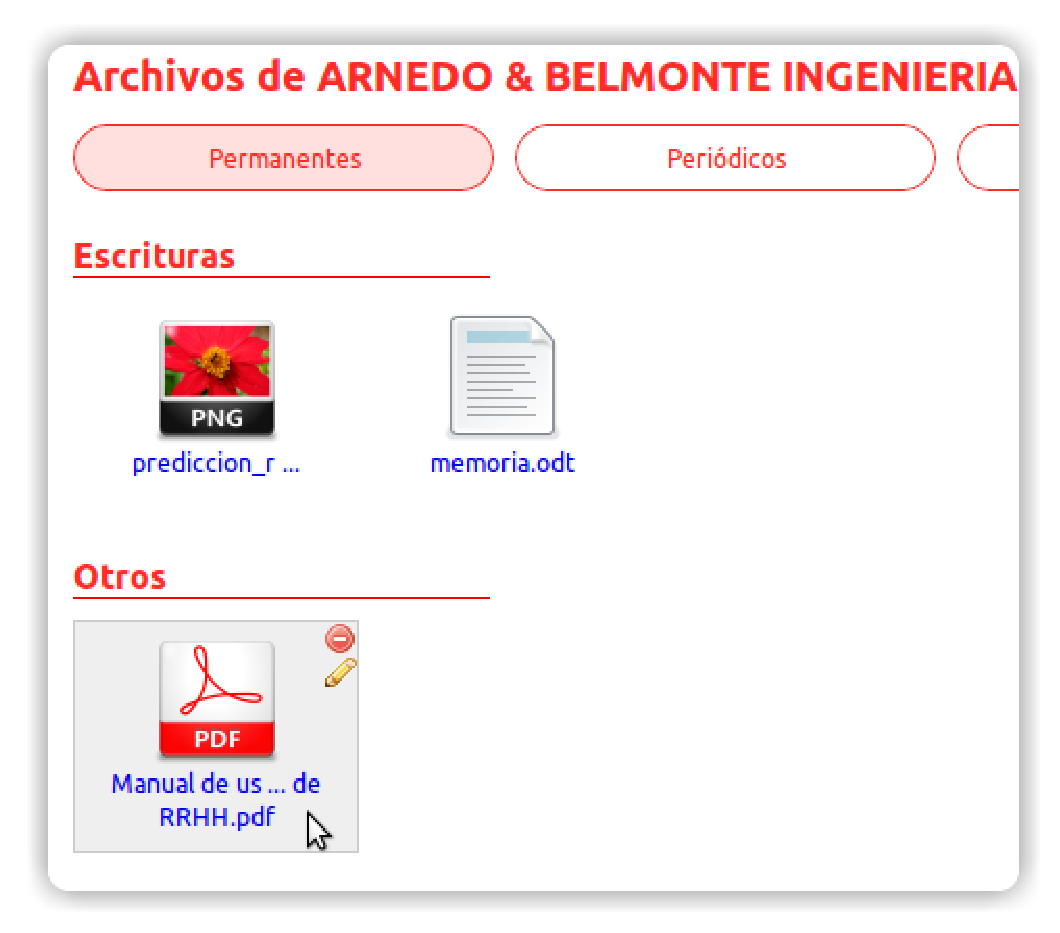
\epsfig{file=imagenes/otrosproyectos/archivos,width=3.5in}
\caption{Gestor de archivos.}
\label{fig:archivos}
\end{figure}


\begin{figure}
\centering
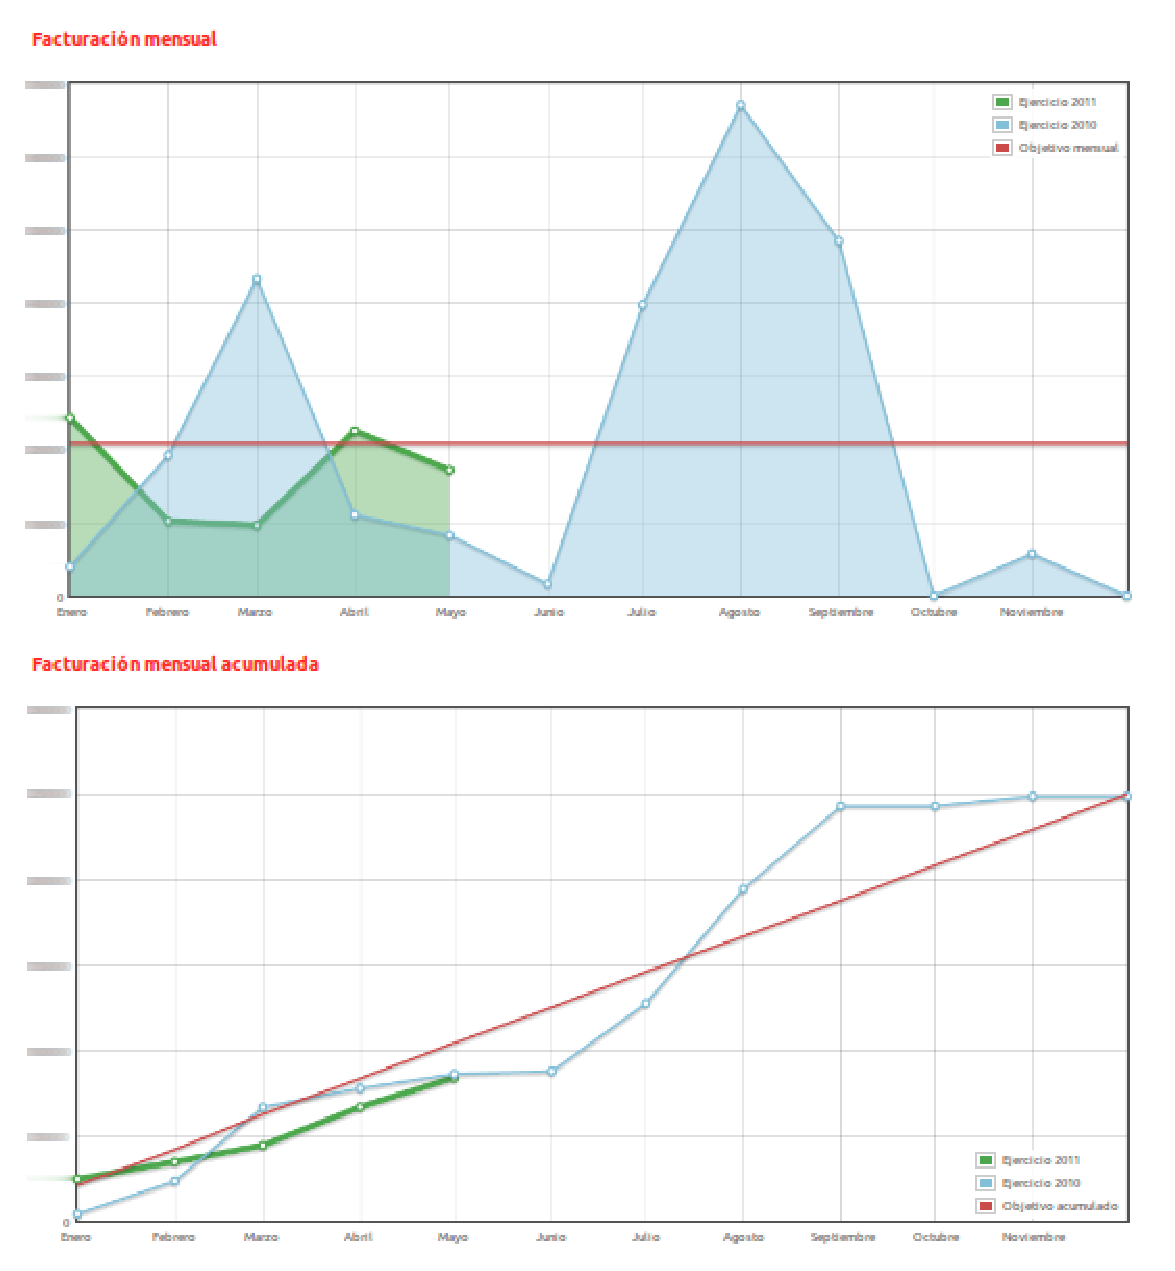
\epsfig{file=imagenes/otrosproyectos/facturacion,width=3.5in}
\caption{Facturación comparada mensual (arriba) y acumulada.}
\label{fig:facturacion}
\end{figure}


\begin{thebibliography}{50}

\bibitem{glass04}
  Michael Glass y otros,
  \emph{Desarrollo web con PHP, Apache y MySQL}.
  Anaya Multimedia, Madrid,
  2004.

\bibitem{rosebrock04}
   Eric Rosebrock, Eric Filson,
  \emph{Setting up LAMP : getting Linux, Apache, MySQL, and PHP working
together}.
  Sybex, San Francisco,
  2004.

\bibitem{date09}
   C.J. Date,
  \emph{SQL and relational theory : how to write accurate SQL code}.
  O'Reilly, Sebastopol,
  2009.

\bibitem{meloni08}
   Julie C. Meloni,
  \emph{PHP, MySQL y Apache}.
  Anaya Multimedia, Madrid,
  2008.

\bibitem{cascales00}
  Bernardo Cascales Salinas,
  \emph{\LaTeX: una imprenta en sus manos}.
  Aula Documental de Investigación, Madrid,
  2000.

\bibitem{lamport94}
  Leslie Lamport,
  \emph{\LaTeX: A Document Preparation System}.
  Addison Wesley, Massachusetts,
  1994.

\end{thebibliography}

\appendix

\chapter{Script del test de distribución de horas}
\label{apx:script_distribucion}
\thispagestyle{empty}
\lstinputlisting{distribucion/distribucion.php}


\chapter{Declaración del cliente}
\label{apx:declaracion_cliente}
\thispagestyle{empty}
Desde \textsc{Arnedo \& Belmonte Ingeniería e Innovación S.L.}, y en su nombre,
Sonia Belmonte y León Arnedo, deseamos expresar nuestra satisfacción con la
herramienta desarrollada por Javier Cejudo para su proyecto ``Herramienta de
apoyo para la gestión de recursos humanos en el desarrollo de proyectos de
I+D''.

Cuando conocimos que la Agencia de Desarrollo Económico de La Rioja (ADER) iba a
cambiar la forma en que se debían justificar los proyectos de I+D, encontramos
que la adaptación de la metodología que veníamos empleando durante los pasados
años era poco menos que impracticable.

Al disponer de una base de datos de clientes y proyectos, entre otras cosas,
surgió la posibilidad de integrar la gestión de las justificaciones con la
\textit{intranet} de la empresa. Dadas nuestras actividades principales,
focalizadas en la consultoría, no disponíamos de un programador en la plantilla
que pudiera llevar a cabo esta labor.

Anteriormente, habíamos colaborado con el Servicio de Relaciones con la Empresa
(SRE) de la Universidad de La Rioja a través de la Oficina de Orientación
Profesional y Empleo (OPE), recibiendo sobre todo a estudiantes de las ramas de
Ingeniería Industrial. Los buenos resultados de esta colaboración nos animaron
a solicitar un estudiante de Ingeniería Informática.

Las labores de Javier Cejudo fueron diversas durante su periodo de prácticas,
e incluyeron el desarrollo de este proyecto, que solo se convirtió en su PFC
(Proyecto Fin de Carrera) cuando se supo lo suficientemente complejo.

En este sentido, nos gustaría expresar la notable utilidad del proyecto,
confirmar que se ha venido usando desde su finalización y que se seguirá usando
y, probablemente, ampliando en el futuro.

\quad

% Author and supervisor
\begin{minipage}{0.4\textwidth}
\begin{flushleft}
\emph{Socia fundadora:}\\
Sonia \textsc{Belmonte}
\end{flushleft}
\end{minipage}
\begin{minipage}{0.4\textwidth}
\begin{flushright}
\emph{Socio fundador:} \\
León \textsc{Arnedo}
\end{flushright}
\end{minipage}

\vfill

% Bottom of the page
En Logroño, a \today


\chapter{Manual de usuario}
\label{apx:manual_usuario}
\thispagestyle{empty}

Este manual abarca toda la funcionalidad de la herramienta en cuanto a gestión
de personal, actividades y a la interacción ambos, aparte de los informes que
pueden generarse. El acceso a la aplicación no forma parte de este manual, por
lo que deberá consultarse el manual de usuario existente antes de que se
introdujeran las nuevas funcionalidades.

\section{Gestión de personal}
\label{sec:manual_personal}

Para una gestión integral del personal, debemos ser capaces de introducir nuevo
personal, modificar personal existente y borrar personal. Parte de su
información varía de forma periódica, en general, anualmente, por lo que
también se guiará a través del proceso de gestión de esta información.

Para comenzar a gestionar recursos, lo primero que debemos hacer es seleccionar
la entrada del menú con el nombre \textbf{Personal}, como se ve en la figura
\ref{fig:inicio_manual}.

\begin{figure}
\centering
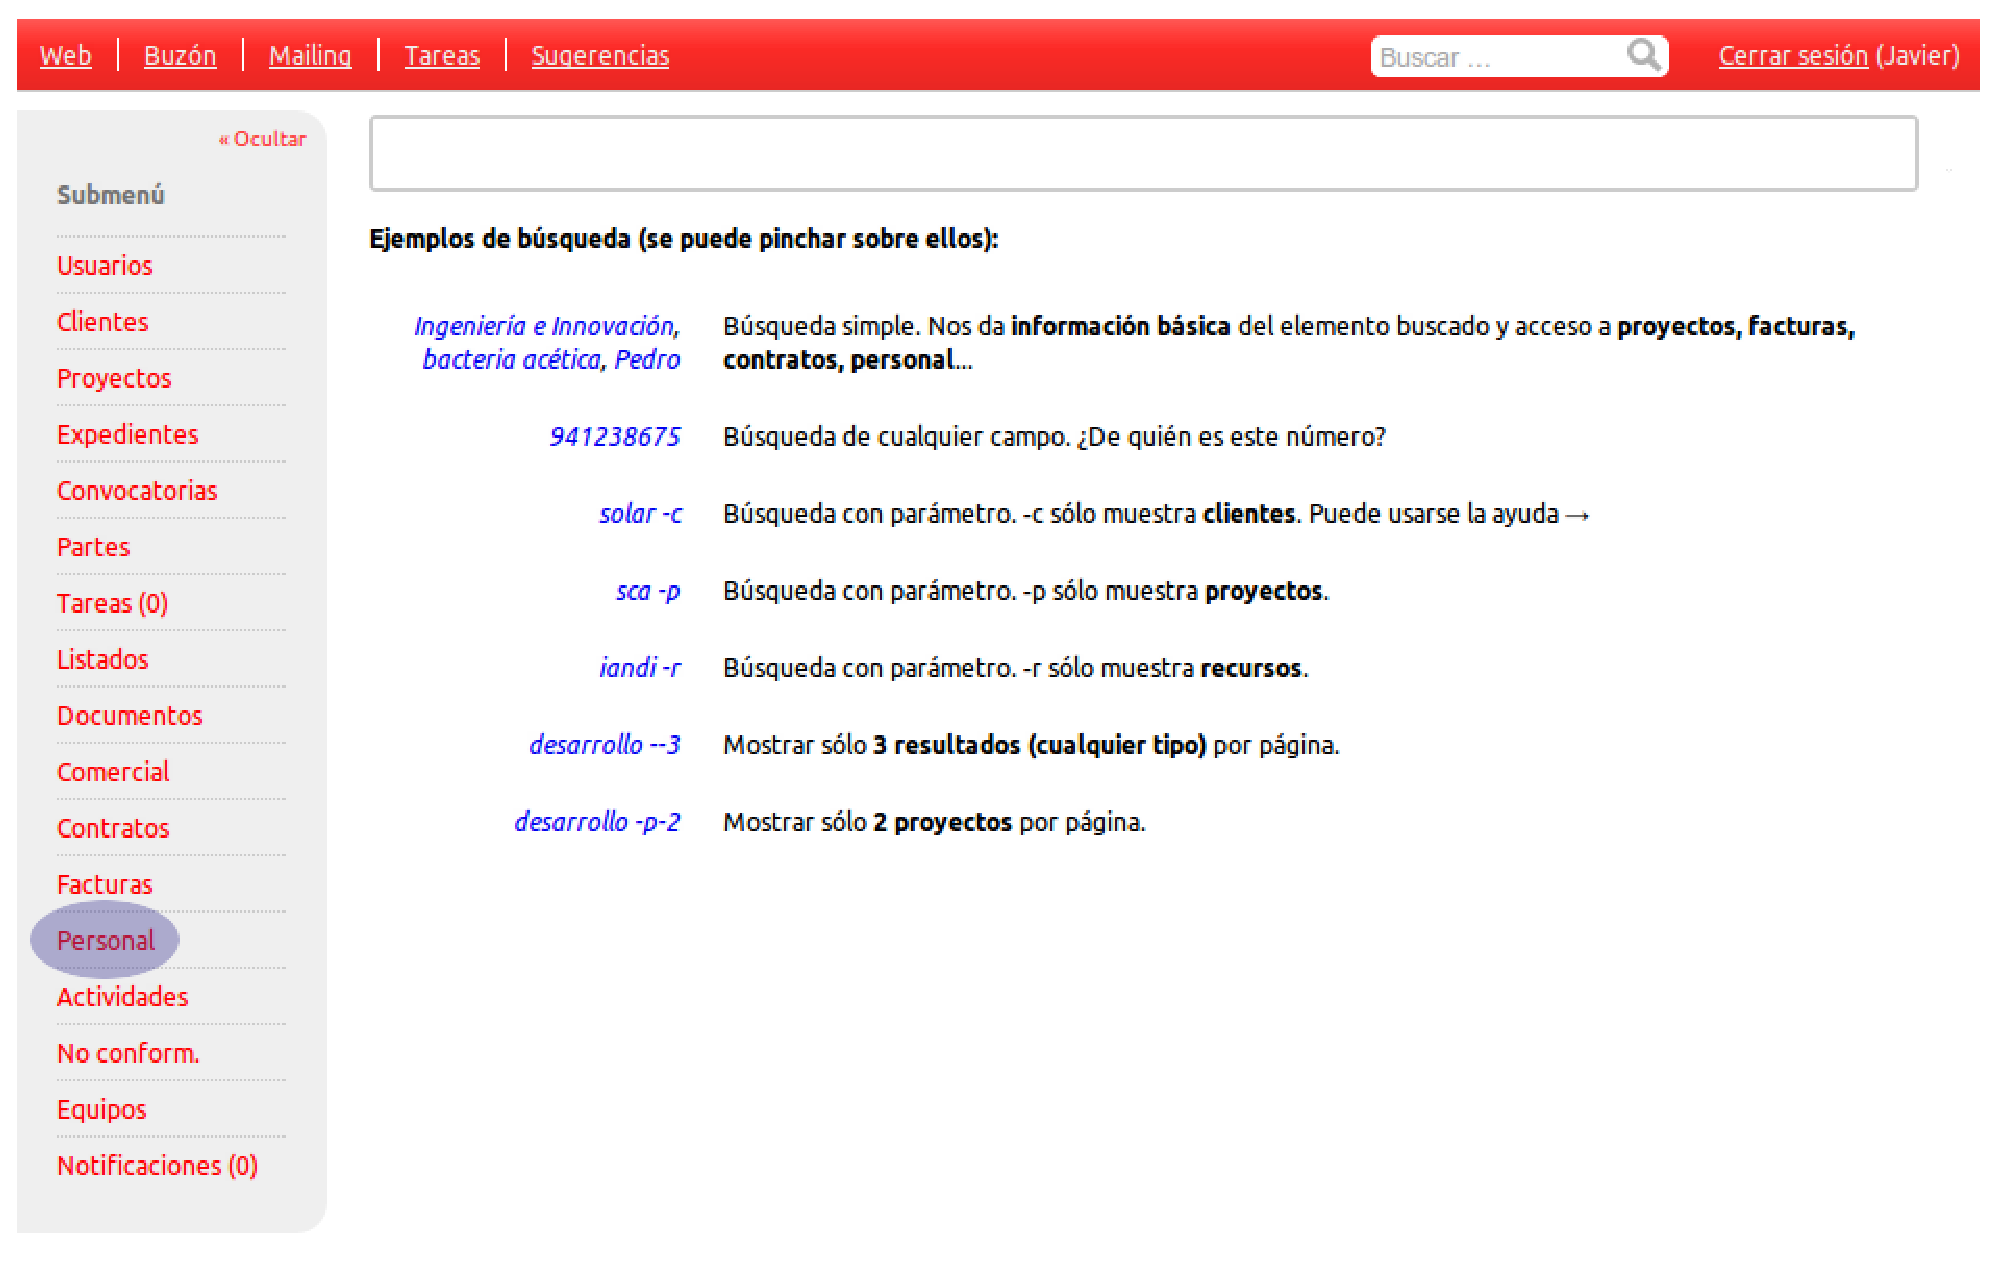
\epsfig{file=imagenes/manual/inicio,width=5.28in}
\caption{Enlace al módulo de personal en el menú.}
\label{fig:inicio_manual}
\end{figure}

\subsection{Búsqueda de personal}
\label{sec:manual_busqueda_personal}

Lo primero que nos encontramos es un buscador de personal (figura
\ref{fig:filtro_personal}), que funciona más propiamente como un filtro: esto
quiere decir que si no introducimos ningún valor y pulsamos \textbf{Buscar}, se
nos mostrarán todos los empleados de todas las empresas.

\begin{figure}
\centering
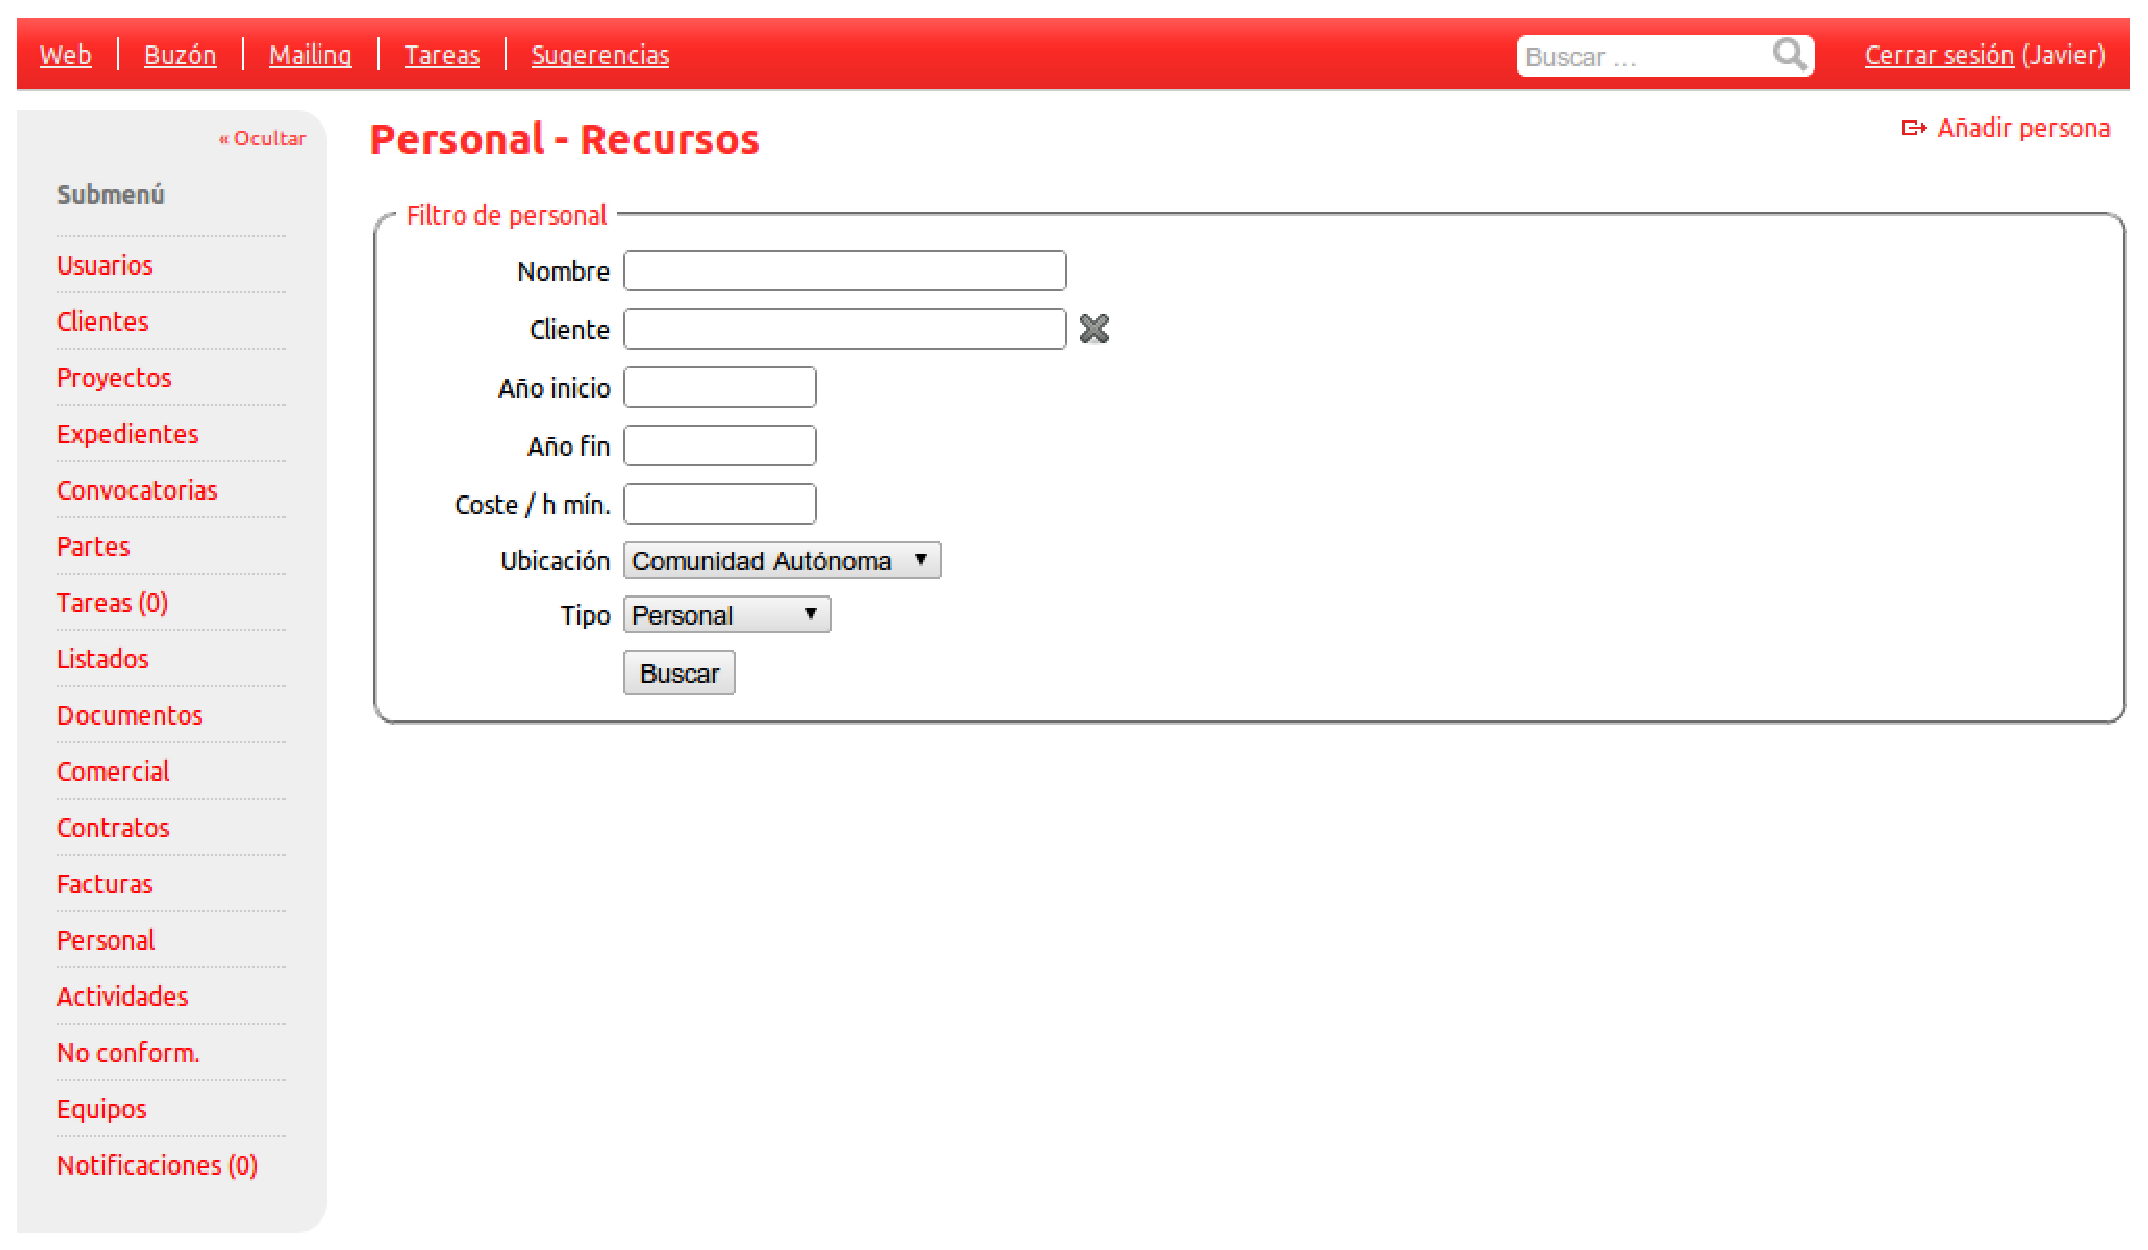
\epsfig{file=imagenes/manual/filtro_personal,width=5.28in}
\caption{Filtro de personal.}
\label{fig:filtro_personal}
\end{figure}

Sin embargo, en general, solo queremos localizar un empleado concreto o
empleados de un mismo cliente, por lo que podemos hacer uso de cualquiera
combinación de los campos del filtro:

\begin{description}
 \item[Nombre] La búsqueda por nombre nos devuelve cualquier empleado cuyo
nombre contenga la cadena introducida.
 \item[Cliente] La búsqueda por cliente es un poco más sofisticada: cuando
introducimos más de tres caracteres, se nos sugieren hasta 20 clientes que
pueden tener relación con la cadena introducida, ya sea por su nombre o
acrónimo (figura \ref{fig:sug_cliente}). Si seleccionamos una de esas
sugerencias, la aplicación deja de usar la cadena como referencia en favor del
identificador del cliente y nos devolverá únicamente los empleados de ese
cliente, al margen de que otros clientes también satisfagan la cadena
introducida.
  \begin{figure}
  \centering
  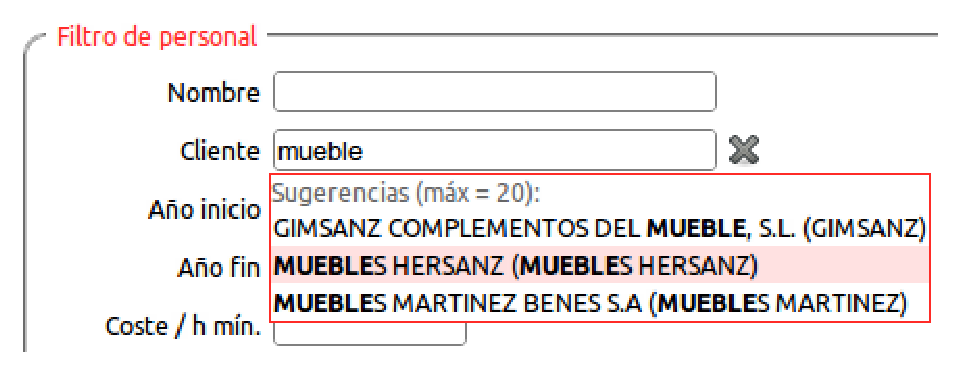
\epsfig{file=imagenes/manual/sug_cliente,width=3.96in}
  \caption{Sugerencias de cliente.}
  \label{fig:sug_cliente}
  \end{figure}
 \item[Año inicio / Año fin] Si los empleados de una empresa llevan muchos años
trabajando, puede que no nos interese conocer los datos que se refieren a hace
más de 5 años, o puede que estemos buscando aquellos precisamente.
 \item[Coste por hora mínimo] Este apartado sirve para encontrar a los
empleados que ganan más de un determinado valor, lo que puede ser interesante a
la hora de planificar proyectos, implicando a trabajadores que ganan más para
obtener una subvención mayor.
 \item[Ubicación] Se refiere a la Comunidad Autónoma de procedencia del
empleado. Especialmente útil para localizar empleados de una de las sedes de
los clientes intercomunitarios.

\end{description}

\subsection{Creación de un nuevo empleado y de sus datos anuales}

Para crear un nuevo empleado, basta con hacer clic en el enlace que aparece en
la esquina superior derecha de cualquier página del módulo de \textbf{Personal}
(figura \ref{fig:aniadir_persona}).

\begin{figure}
\centering
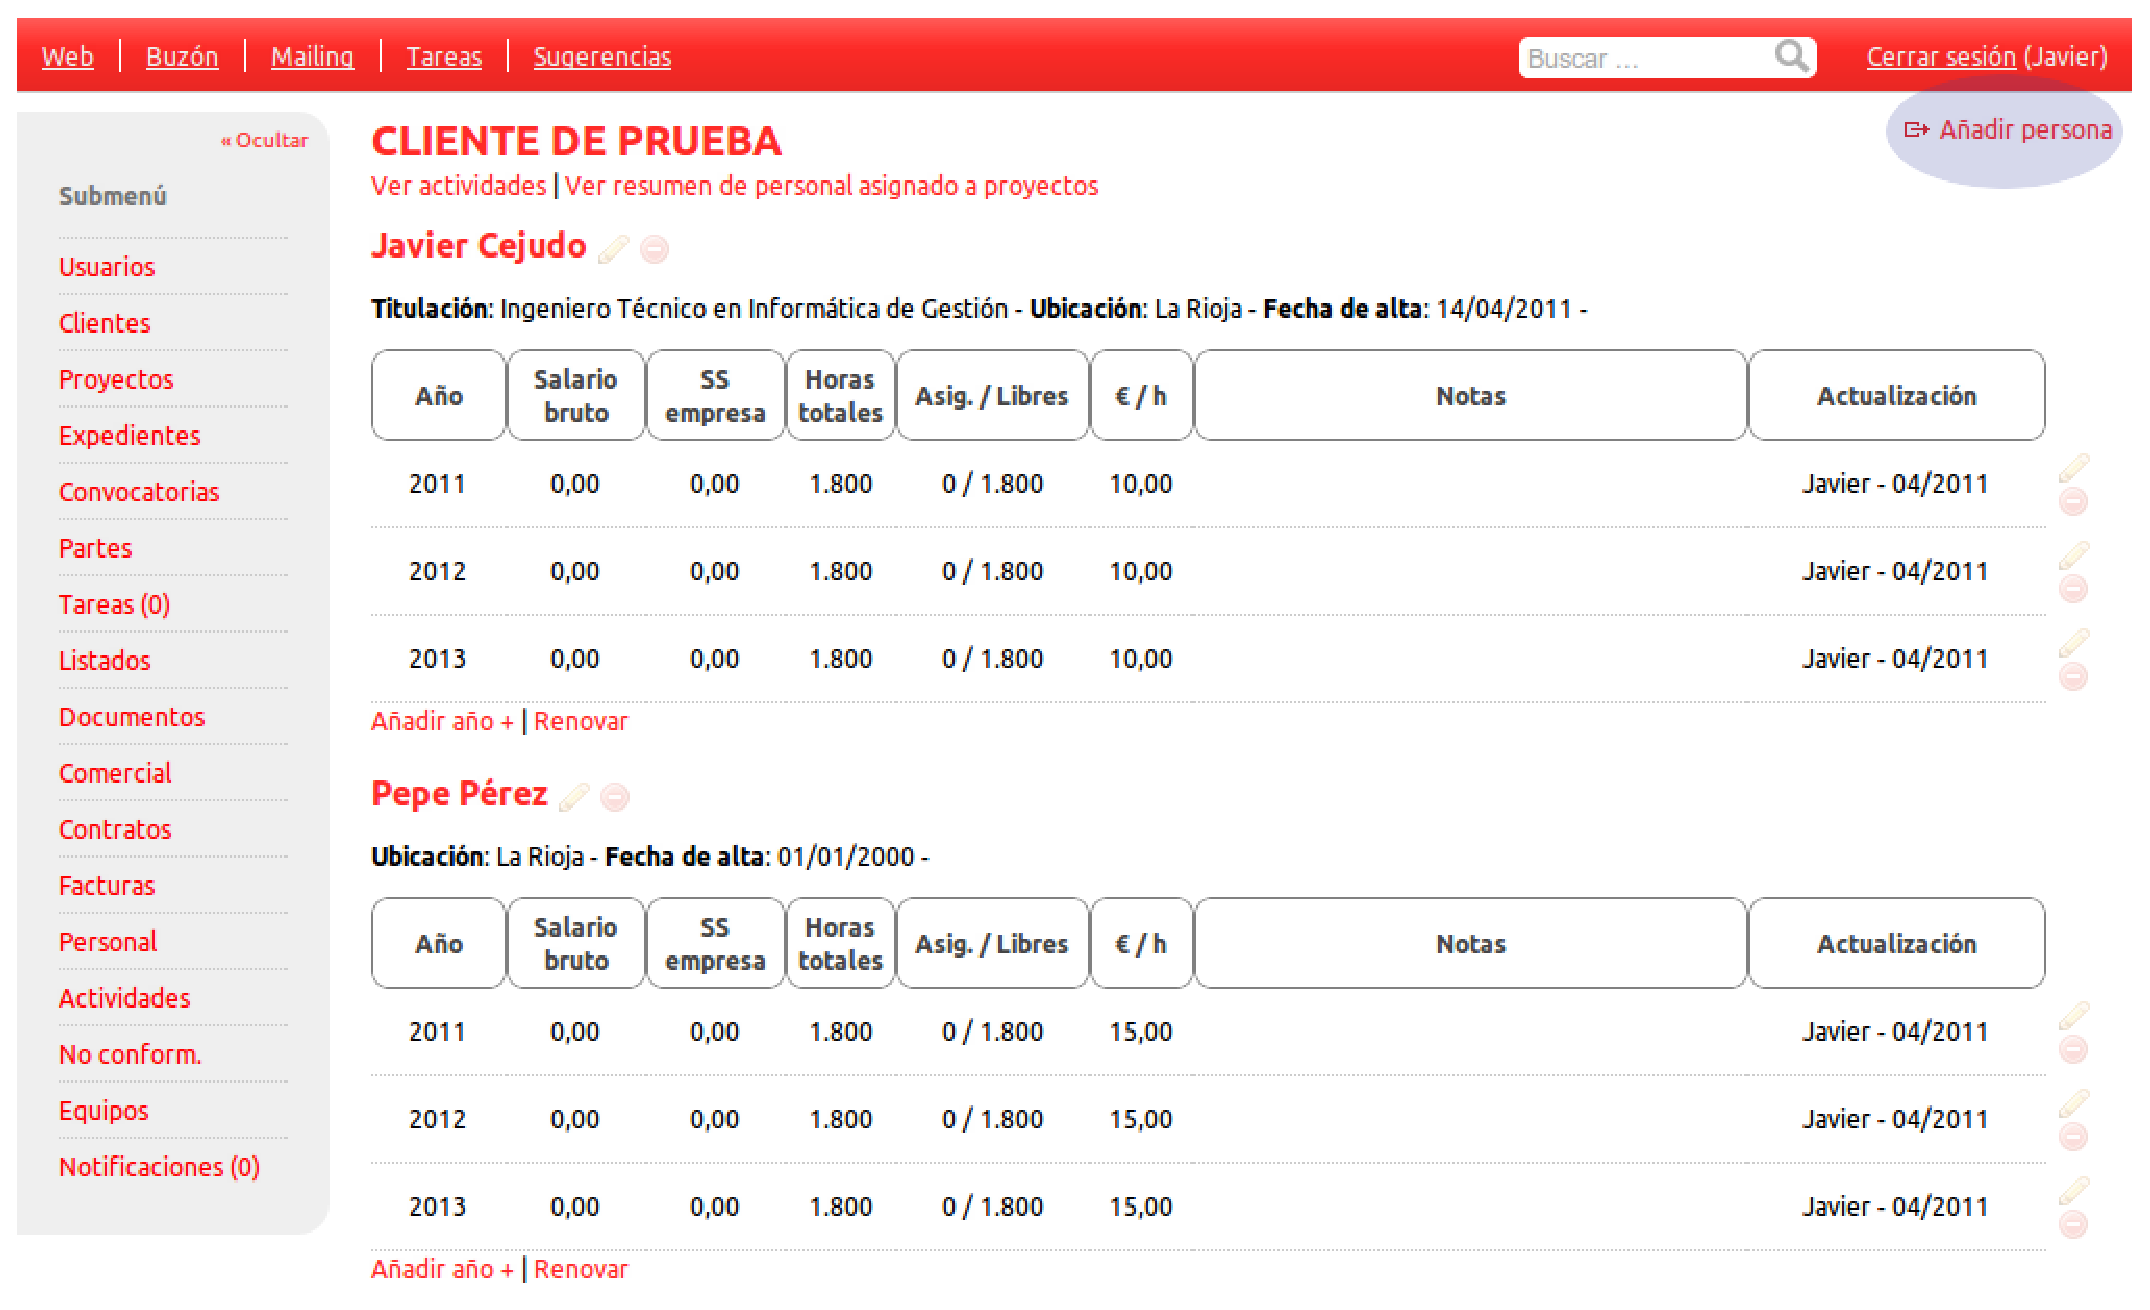
\epsfig{file=imagenes/manual/aniadir_persona,width=5.28in}
\caption{Enlace para añadir personal.}
\label{fig:aniadir_persona}
\end{figure}

Una vez hemos pinchado en el enlace, nos aparecerá el formulario de la figura
\ref{fig:form_personal}, que debemos rellenar, al menos, con los datos
obligatorios: nombre y cliente. Cabe destacar que si hemos realizado una
búsqueda para un cliente concreto, el enlace a \textbf{Añadir persona} pasa la
información del cliente al formulario, por lo que simplemente añadiendo un
nombre, ya tendríamos un empleado nuevo. Siempre podemos modificar los datos
más adelante, como se indica en este mismo manual.

\begin{figure}
\centering
\epsfig{file=imagenes/manual/form_personal,width=4in}
\caption{Creación de nuevo personal.}
\label{fig:form_personal}
\end{figure}

Una vez rellenado el formulario, hay que enviar los datos. Vemos que el enlace
para enviar el formulario dice \textbf{Crear y añadir datos anuales}. Esto se
debe a que un empleado sin datos anuales no es interesante para la aplicación,
ya que no podríamos imputarle horas. El formulario para los datos anuales se
puede ver en la figura \ref{fig:form_anuales}.

\begin{figure}
\centering
\epsfig{file=imagenes/manual/form_anuales,width=4in}
\caption{Creación de datos anuales.}
\label{fig:form_anuales}
\end{figure}

Los datos obligatorios de este formulario son el \textbf{año} y el
\textbf{coste/hora}; sin embargo, si tenemos los datos acerca del salario
bruto, la Seguridad Social a cargo de la empresa y las horas anuales del
convenio, el coste/hora se calculará automáticamente.

Para añadir más datos anuales, podemos hacer clic en los enlaces que aparecen
debajo de la tabla de datos anuales de cada empleado (figura
\ref{fig:aniadir_anuales}).

\begin{figure}
\centering
\epsfig{file=imagenes/manual/aniadir_anuales,width=3in}
\caption{Enlaces para añadir datos anuales.}
\label{fig:aniadir_anuales}
\end{figure}

\begin{description}
 \item [Añadir año +] Este enlace nos lleva al mismo formulario de la figura
\ref{fig:form_anuales}, pero nos sugiere un valor de horas anuales basándose en
años anteriores o en datos de otros empleados.
 \item [Renovar] Este enlace añade automáticamente el año inmediatamente
posterior al más reciente, tomando como referencia sus datos (horas del
convenio, salario...).
\end{description}

\subsection{Modificación de un empleado y de sus datos anuales}

La necesidad de modificar un empleado es bastante común, ya sea para añadir
datos que se dejaron sin completar en la creación o para actualizar o corregir
datos erróneos. Esta acción se puede llevar a cabo fácilmente haciendo clic en
el icono que representa un lapicero, y que se puede encontrar al lado del
nombre del empleado (figura \ref{fig:mod_persona}).

\begin{figure}
\centering
\epsfig{file=imagenes/manual/mod_persona,width=3in}
\caption{Enlace para modificar los datos de un empleado.}
\label{fig:mod_persona}
\end{figure}

Entonces, nos aparecerá un formulario con los datos actuales del empleado
(figura \ref{fig:form_mod_persona}), que podemos modificar con la nueva
información de la que disponemos. Cabe destacar que no puede modificarse el
cliente al que pertenece el empleado debido a que podría tener horas imputadas
con el cliente actual y crearse inconsistencias.

\begin{figure}
\centering
\epsfig{file=imagenes/manual/form_mod_persona,width=5.28in}
\caption{Formulario de modificación de empleados.}
\label{fig:form_mod_persona}
\end{figure}

Los datos anuales pueden modificarse desde los enlaces de la parte derecha de
la tabla de datos anuales. El icono para modificar elementos en la aplicación es
siempre un lapicero (figura \ref{fig:mod_anuales}).

\begin{figure}
\centering
\epsfig{file=imagenes/manual/mod_anuales,width=2.28in}
\caption{Enlace para modificar datos anuales.}
\label{fig:mod_anuales}
\end{figure}

En el formulario de modificación de datos anuales (figura
\ref{fig:form_mod_anuales}), podemos modificar cualquier valor excepto el año,
debido a que una modificación de ese tipo lleva implícita la desaparición de un
año al que se pueden haber imputado horas.

\begin{figure}
\centering
\epsfig{file=imagenes/manual/form_mod_anuales,width=3.64in}
\caption{Formulario de modificación de empleados.}
\label{fig:form_mod_anuales}
\end{figure}

\subsection{Eliminación de un empleado y de sus datos anuales}

La eliminación de empleados y de sus datos anuales son acciones de alto riesgo.
Cualquiera de estas acciones borraría a su vez las decenas sino cientos de
datos referentes a horas imputadas del empleado. Es por ello que estas acciones
solamente pueden ser llevadas a cabo por el usuario Administrador. La
disposición de los iconos es totalmente análoga a la de modificación de
personal (figuras \ref{fig:bor_persona} y \ref{fig:bor_anuales}). En cualquier
caso, se nos pedirá confirmar la acción.

\begin{figure}
\centering
\epsfig{file=imagenes/manual/bor_persona,width=3in}
\caption{Enlace para borrar los datos de un empleado.}
\label{fig:bor_persona}
\end{figure}

\begin{figure}
\centering
\epsfig{file=imagenes/manual/bor_anuales,width=2.28in}
\caption{Enlace para borrar datos anuales.}
\label{fig:bor_anuales}
\end{figure}


% % % % % % % % % % % % % % % % % % % % % % % % % % % % % % % % % % % %
% % % % % % % % % % % % % % % % % % % % % % % % % % % % % % % % % % % %

% % % % % % % % % % % % % % % % % % % % % % % % % % % % % % % % % % % %
% % % % % % % % % % % % % % % % % % % % % % % % % % % % % % % % % % % %

% % % % % % % % % % % % % % % % % % % % % % % % % % % % % % % % % % % %
% % % % % % % % % % % % % % % % % % % % % % % % % % % % % % % % % % % %


\section{Gestión de actividades}
\label{sec:manual_actividades}

Para una gestión integral de las actividades, debemos ser capaces de crear
nuevas actividades, modificar actividades existentes y borrar actividades. Las
actividades deben formar parte de un proyecto y solo de un proyecto.

Para comenzar a gestionar actividades, lo primero que debemos hacer es
seleccionar la entrada del menú con el nombre \textbf{Actividades}, como se ve
en la figura \ref{fig:inicio_act}.

\begin{figure}
\centering
\epsfig{file=imagenes/manual/inicio_act,width=5.28in}
\caption{Enlace al módulo de actividades en el menú.}
\label{fig:inicio_act}
\end{figure}

\subsection{Búsqueda de proyectos/actividades}
\label{sec:manual_busqueda_actividades}

Lo primero que nos encontramos es un buscador de actividades (figura
\ref{fig:filtro_act}), que funciona más propiamente como un filtro: esto
quiere decir que si no introducimos ningún valor y pulsamos \textbf{Buscar}, se
nos mostrarán todas las actividades de todos los proyectos.

\begin{figure}
\centering
\epsfig{file=imagenes/manual/filtro_act,width=5.28in}
\caption{Filtro de actividades.}
\label{fig:filtro_act}
\end{figure}

Sin embargo, en general, solo queremos localizar una actividad concreta o
todas las actividades de un mismo proyecto, por lo que podemos hacer uso de
cualquiera combinación de los campos del filtro:

\begin{description}
 \item[Proyecto] La búsqueda por cliente es más o menos sofisticada: cuando
introducimos más de tres caracteres, se nos sugieren hasta 20 proyectos que
pueden tener relación con la cadena introducida, ya sea por su nombre o
acrónimo (figura \ref{fig:sug_proyecto}) o por el nombre o acrónimo del cliente.
Si seleccionamos una de esas sugerencias, la aplicación deja de usar la cadena
como referencia en favor del identificador del proyecto y nos devolverá
únicamente los proyectos y las actividades de ese cliente, al margen de que
otros proyectos también satisfagan la cadena introducida.
  \begin{figure}
  \centering
  \epsfig{file=imagenes/manual/sug_proyecto,width=3.88in}
  \caption{Sugerencias de proyecto.}
  \label{fig:sug_proyecto}
  \end{figure}
 \item[Cliente] La búsqueda por cliente funciona exactamente igual que en el
filtro de personal (figura \ref{fig:sug_cliente}).
 \item[Nombre] La búsqueda por nombre nos devuelve cualquier actividad cuyo
nombre contenga la cadena introducida.

\end{description}

\subsection{Creación de una nueva actividad}

Para crear una nueva actividad, basta con hacer clic en el enlace que aparece en
la esquina superior derecha de cualquier página del módulo de
\textbf{Actividades} o bien al final de la lista de actividades de cada
proyecto (figura \ref{fig:aniadir_actividad}).

\begin{figure}
\centering
\epsfig{file=imagenes/manual/aniadir_actividad,width=5.28in}
\caption{Enlaces para añadir actividades.}
\label{fig:aniadir_actividad}
\end{figure}

Una vez hemos pinchado en el enlace, nos aparecerá el formulario de la figura
\ref{fig:form_actividad}, que debemos rellenar, al menos, con los datos
obligatorios: proyecto, nombre, fecha de inicio y fecha de fin. Cabe destacar
que si hemos realizado una búsqueda para un proyecto concreto o si pinchamos el
enlace bajo la lista de actividades de un proyecto, el campo proyecto
aparecerá rellenado.

\begin{figure}
\centering
\epsfig{file=imagenes/manual/form_actividad,width=4.21in}
\caption{Creación de nueva actividad.}
\label{fig:form_actividad}
\end{figure}


\subsection{Modificación de una actividad}

La necesidad de modificar una actividad es relativamente común, a pesar de que
la mayoría de los proyectos están plenamente planificados desde el inicio. Las
principales modificaciones se deben a desfases temporales en la ejecución de
proyecto. Esta acción se puede llevar a cabo fácilmente haciendo clic en el
icono que representa un lapicero, y que se puede encontrar en la parte de la
derecha de la tabla de actividades de cada proyecto (figura
\ref{fig:mod_actividad}).

\begin{figure}
\centering
\epsfig{file=imagenes/manual/mod_actividad,width=2.23in}
\caption{Enlace para modificar los datos de una actividad.}
\label{fig:mod_actividad}
\end{figure}

Entonces, nos aparecerá un formulario con los datos actuales de la actividad
(figura \ref{fig:form_mod_actividad}), que podemos modificar con la nueva
información de la que disponemos. Cabe destacar que no puede modificarse el
proyecto al que pertenece el empleado debido a que podría haber horas imputadas
con el proyecto actual y crearse inconsistencias.

\begin{figure}
\centering
\epsfig{file=imagenes/manual/form_mod_actividad,width=5.28in}
\caption{Formulario de modificación de empleados.}
\label{fig:form_mod_actividad}
\end{figure}

\subsection{Eliminación de una actividad}

La eliminación de actividades es una acción de alto riesgo, ya que con cada
actividad borrada, se pierden a su vez las decenas sino cientos de datos
referentes a horas imputadas. Es por ello que la eliminación de actividades
solamente puede ser llevada a cabo por el usuario Administrador. La
disposición de los iconos es totalmente análoga a la de modificación de
actividades (figura \ref{fig:bor_actividad}). En cualquier caso, se nos pedirá
confirmar la acción.

\begin{figure}
\centering
\epsfig{file=imagenes/manual/bor_actividad,width=2.23in}
\caption{Enlace para borrar una actividad.}
\label{fig:bor_actividad}
\end{figure}

\section{Consulta de datos e informes}

La consulta de datos va a ser nuestra principal actividad como usuarios del
sistema, de modo que es importante que conozcamos todas las posibilidades que
este nos ofrece.

La consulta de personal y actividades se ha descrito en secciones
anteriores de este manual (\ref{sec:manual_personal},
\ref{sec:manual_actividades}), de manera que nos centraremos en la consulta de
horas asignadas, cuya gestión se describirá, a su vez, en la sección siguiente
(sección \ref{sec:manual_horas}).

La primera pregunta que nos debemos hacer es si estamos interesados en conocer
las horas asignadas a un recurso independientemente de los proyectos
involucrados, a un proyecto independientemente de los recursos asignados, o más
bien buscamos datos concretos sin \textit{variables libres}.

\subsection{Consulta de datos por personal}

La forma más rápida de conocer cuántas horas tiene asignadas un recurso en un
año concreto, es buscar a ese recurso como se explicó en la sección
\ref{sec:manual_busqueda_personal} y revisar sus horas asignadas anualmente
como se indica en la figura \ref{fig:horas_anuales}.

\begin{figure}
\centering
\epsfig{file=imagenes/manual/horas_anuales,width=4.73in}
\caption{Horas asignadas a un empleado concreto en 2010 y 2011.}
\label{fig:horas_anuales}
\end{figure}

Cualquier valor de horas con la apariencia usual de los enlaces en la web es,
de hecho, un enlace a un informe desglosado por meses de esas horas. Así,
pinchando en el segundo de los valores señalados en la figura
\ref{fig:horas_anuales}, obtendremos el desglose de la figura
\ref{fig:desglose_horas}. En el filtro superior del desglose, que podemos
modificar a nuestro antojo, se aprecia que no hay seleccionado ningún proyecto,
y de hecho, vemos que están mezcladas las horas de dos proyectos: PRUEBA y
PRUEBA2.

\begin{figure}
\centering
\epsfig{file=imagenes/manual/desglose_horas,width=4.5in}
\caption{Desglose mensual de horas para un recurso concreto.}
\label{fig:desglose_horas}
\end{figure}

\subsection{Consulta de datos por proyecto}

La forma más rápida de conocer cuántas horas hay asignadas a un proyecto
concreto, es buscar ese proyecto como se explicó en la sección
\ref{sec:manual_busqueda_actividades}. En la página de cada proyecto,
encontraremos los siguientes informes:

\begin{description}
 \item [Desglose general por actividades (figura \ref{fig:consulta_horas_act})]
Este informe no identifica personal y su principal uso será la gestión de
actividades, más que la consulta de horas.
 \item [Resumen de horas por año (figura \ref{fig:horas_resumen_anio})] Muestra
el sumatorio de horas por año para cada empleado en las tres fases de la gestión
de los proyectos: presentación, aprobación y justificación.
 \item [Resumen de horas por actividad (figura
\ref{fig:horas_resumen_actividad})] Muestra el sumatorio de horas por actividad
para cada empleado en las tres fases de la gestión de los proyectos:
presentación, aprobación y justificación.

\end{description}

\begin{figure}
\centering
\epsfig{file=imagenes/manual/consulta_horas_act,width=5.28in}
\caption{Desglose general por actividades.}
\label{fig:consulta_horas_act}
\end{figure}

\begin{figure}
\centering
\epsfig{file=imagenes/manual/horas_resumen_anio,width=5.28in}
\caption{Resumen de horas por año.}
\label{fig:horas_resumen_anio}
\end{figure}

\begin{figure}
\centering
\epsfig{file=imagenes/manual/horas_resumen_actividad,width=5.28in}
\caption{Resumen de horas por año.}
\label{fig:horas_resumen_actividad}
\end{figure}

A partir de los enlaces de cada valor, podemos acceder al desglose mensual
(figura \ref{fig:desglose_horas}) y ajustar el filtro para nuestras necesidades
en cada momento; así, por ejemplo, podríamos seleccionar todos los empleados y
un proyecto o actividades concretos.

Adicionalmente, existe la posibilidad de descargar (figura
\ref{fig:enlace_resumen}) una hoja de cálculo con la información de cada
empleado acerca de su participación en el proyecto para su etapa de
presentación, aprobación o justificación. La hoja de cálculo tiene tantas hojas
como empleados participan en el proyecto, y tiene el aspecto de la figura
\ref{fig:hoja_calculo_proyecto}.

\begin{figure}
\centering
\epsfig{file=imagenes/manual/enlace_resumen,width=5.28in}
\caption{Enlace a las hojas de cálculo.}
\label{fig:enlace_resumen}
\end{figure}

\begin{figure}
\centering
\epsfig{file=imagenes/manual/hoja_calculo_proyecto,width=5.28in}
\caption{Hoja de cálculo por proyecto, personal, actividades y meses.}
\label{fig:hoja_calculo_proyecto}
\end{figure}

\subsection{Resumen global}

Se puede acceder a un resumen global desde cualquier parte de los módulos de
\textbf{Personal} y \textbf{Actividades}, como se ve en la figura
\ref{fig:enlace_resumen_global_mont}, desde la que también se aprecia que se
puede pasar fácilmente de las actividades de un cliente a su personal y
viceversa.

\begin{figure}
\centering
\epsfig{file=imagenes/manual/enlace_resumen_global_mont,width=5.28in}
\caption{Enlaces al resumen desde Proyectos (izq.) y personal (dcha.).}
\label{fig:enlace_resumen_global_mont}
\end{figure}

El objetivo del resumen global (figura
\ref{fig:resumen_horas_asignadas_proyectos}) es que sea posible, de un vistazo,
obtener la mayor cantidad de información posible:

\begin{itemize}
\item puede identificarse cuándo un empleado no está dado de alta en la
empresa.

\item se tiene en cuenta el convenio de horas del recurso para informar acerca
de las horas que le quedan libres en un año;

\item cuando existe un conflicto, por ejemplo, se hayan imputado más horas
de las que deberían, el valor aparece marcado en rojo;

\item las columnas de proyectos siguen un código de colores para indicar el
estado en que se encuentra el proyecto;

\item cada uno de los valores, incluidos los nombres de los recursos en
cuestión, son un enlace a otra vista donde se darán detalles acerca
del elemento (la figura \ref{fig:desglose_mensual_actividades} es el desglose
de las horas marcadas en la figura \ref{fig:resumen_horas_asignadas_proyectos}).
En esta vista, también se muestra el coste/hora de
cada empleado para calcular el coste de la selección.
\end{itemize}

\begin{figure}
\centering
\epsfig{file=imagenes/manual/prediccion_resumen,width=5.28in}
\caption{Resumen de horas asignadas a proyectos.}
\label{fig:resumen_horas_asignadas_proyectos}
\end{figure}

\begin{figure}
\centering
\epsfig{file=imagenes/manual/desglose_mensual_actividades,width=5.28in}
\caption{Vista de desglose mensual por actividades.}
\label{fig:desglose_mensual_actividades}
\end{figure}

El resumen global puede descargarse en formato de hoja de cálculo desde el
enlace que figura junto a la leyenda bajo la tabla en sí, y tiene el aspecto de
la figura \ref{fig:hoja_calculo_global}.

\begin{figure}
\centering
\epsfig{file=imagenes/manual/hoja_calculo_global,width=5.28in}
\caption{Resumen global en hoja de cálculo.}
\label{fig:hoja_calculo_global}
\end{figure}

\section{Gestión de horas}
\label{sec:manual_horas}

\subsection{Asignación de horas}

La imputación efectiva de horas se realiza desde el módulo de actividades,
pinchando en el icono que representa a una persona a la derecha de la tabla de
actividades de cada proyecto (figura \ref{fig:asig_horas}).

\begin{figure}
\centering
\epsfig{file=imagenes/manual/asig_horas,width=2.23in}
\caption{Enlace para imputar horas a una actividad.}
\label{fig:asig_horas}
\end{figure}

El formulario de asignación (figura \ref{fig:form_asig_horas}) requiere los
siguientes datos para realizar correctamente la imputación:

\begin{description}
 \item [Persona] Se trata del empleado a quien se desea imputar horas. Se
puede elegir entre un listado que comprende a los empleados del cliente
responsable del proyecto y a los de todos los clientes que figuran como
cooperantes del proyecto.
 \item [Tipo de horas] Se refiere a la naturaleza de las horas a imputar:
presentadas, aprobadas o justificadas.
 \item [Inicio] Se refiere al inicio de las acciones del empleado en la
actividad. Por defecto, se considera la fecha de inicio de la actividad.
 \item [Fin] Se refiere al fin de las acciones del empleado en la
actividad. Por defecto, se considera la fecha de fin de la actividad.
\end{description}

\begin{figure}
\centering
\epsfig{file=imagenes/manual/form_asig_horas,width=5.28in}
\caption{Formulario de asignación de horas a actividad.}
\label{fig:form_asig_horas}
\end{figure}

Sobre el formulario de asignación (figura \ref{fig:form_asig_horas}), se pueden
destacar algunas cosas:

\begin{itemize}
 \item nos da un listado
de los empleados que ya tienen horas imputadas, de manera que se reduzca la
posibilidad duplicar el esfuerzo;
 \item cuando el inicio y final de la actividad se extiende durante varios
años, nos permite, con un clic, seleccionar el año concreto al que queremos
asignar horas.
 \item nos ayuda a calcular el número de horas basándose en el calendario real
de trabajo (teniendo en cuente festivos...) a partir del número de horas que se
calcula que el trabajador empleará al día en esa actividad.
 \item la opción \textit{asignar y seguir} envía los valores pero mantiene el
formulario abierto con los mismos valores. Esto es especialmente útil cuando
estamos asignando horas en la misma actividad a varios empleados.
\end{itemize}

Dado que en muchas ocasiones se aprueban tantas horas como se presentan o
se justifican tantas como se aprueban, existe la posibilidad de trasladar unas
horas al siguiente estado sin necesidad de reasignar las horas de cada empleado.
Esta acción solamente requiere un clic en los botones correspondientes bajo la
lista de actividades (figura \ref{fig:tras_horas}) pero, ya que sobrescribe
cualquier valor que hubiera previamente, solo puede ser ejecutada por el
administrador.

\begin{figure}
\centering
\epsfig{file=imagenes/manual/tras_horas,width=2.23in}
\caption{Botones de traslación de horas.}
\label{fig:tras_horas}
\end{figure}

\subsection{Modificación de horas asignadas}

El método más simple que tenemos para modificar las horas asignadas a un
empleado es sobrescribir, es decir, hacer una asignación sobre un periodo de
tiempo que ya tenía horas asignadas. Otra acción que nos permite realizar la
aplicación es modificar la asignación mensual calculada automáticamente. Para
ello, debemos acceder a la vista de horas por meses desde cualquier enlace de
horas de los módulos de personal o actividades. Una vez allí, basta con pinchar
en cualquier valor por mes para realizar la modificación, como se ve en la
figura \ref{fig:mod_horas_mes}.

\begin{figure}
\centering
\epsfig{file=imagenes/manual/mod_horas_mes,width=4in}
\caption{Modificación de horas mensuales.}
\label{fig:mod_horas_mes}
\end{figure}

La modificación mensual es muy útil para resolver manualmente las
inconsistencias que pudieran haberse creado en los procesos de asignación.

Debe tenerse en cuenta que no pueden asignarse o modificarse horas
\textit{presentadas} a proyectos \textit{aprobados}, ni horas
\textit{presentadas} o \textit{aprobadas} a proyectos \textit{justificados}.
Cuando un proyecto está \textit{concluido}, no se pueden asignar o modificar
horas de ningún tipo.

\subsection{Detección de errores}

La detección de errores no requiere de ninguna acción por parte del usuario.
Cualquier inconsistencia es marcada en rojo automáticamente, a la espera de las
acciones correctoras de los técnicos.

Ya en la propia asignación de horas, el sistema advierte de cuáles son las
inconsistencias que la acción ha provocado. Se puede ver un ejemplo de esto en
la figura \ref{fig:errores_detectados}.

\begin{figure}
\centering
\epsfig{file=imagenes/manual/errores_detectados,width=3in}
\caption{Detección de errores en la asignación.}
\label{fig:errores_detectados}
\end{figure}

Al pinchar en el enlace para ver los detalles, se nos muestra el filtro general
con las opciones apropiadas preseleccionadas para ver los valores en cuestión.
La última columna de la figura \ref{fig:detalles_errores} muestra las horas
sobrantes y nos enlaza al mes en cuestión, independientemente del proyecto, de
manera que sea posible identificar la naturaleza de la inconsistencia: por
ejemplo, solapamiento del trabajo del empleado en varios proyectos.

\begin{figure}
\centering
\epsfig{file=imagenes/manual/detalles_errores,width=5.28in}
\caption{Detalle de los errores con enlace de horas sobrantes.}
\label{fig:detalles_errores}
\end{figure}

\subsection{Eliminación de horas asignadas}

La eliminación de horas asignadas se realiza sobrescribiendo las horas a
eliminar con una asignación de cero horas. Asimismo, pueden eliminarse meses
concretos desde la vista de desglose mensual (figura \ref{fig:mod_horas_mes}),
de nuevo, mediante la asignación de cero horas.

Cualquier eliminación de personal involucrado en un proyecto o de actividades
que se lleven a cabo en el marco del proyecto eliminan, por supuesto, sus
correspondientes horas asignadas.

\section{Buscador global}

El buscador global es la página de inicio de la aplicación, y también está
disponible a lo largo de toda la sesión en la barra de menú superior (figuras
\ref{fig:buscador_inicio} y \ref{fig:buscador_superior}).

\begin{figure}
\centering
\epsfig{file=imagenes/manual/buscador_inicio,width=5.28in}
\caption{Buscador con ejemplos de uso.}
\label{fig:buscador_inicio}
\end{figure}

\begin{figure}
\centering
\epsfig{file=imagenes/manual/buscador_superior,width=5.28in}
\caption{Posición del buscador en el menú superior.}
\label{fig:buscador_superior}
\end{figure}

Nos permite buscar clientes, recursos humanos y proyectos. Su funcionalidad
general puede describirse con los ejemplos del cuadro
\ref{cua:buscador_opciones}. Para buscar, solamente es necesario comenzar a
teclear en la caja del buscador; los resultados irán apareciendo y
actualizándose mientras sigamos tecleando.

\begin{table}
\centering
\begin{tabular}{|p{1.28in}|p{4in}|}\hline
Consulta & Descripción / Resultado \\\hline\hline
Ingeniería e Innovación, bacteria acética, Pedro & Búsqueda simple. Nos da
información básica del elemento buscado y acceso a proyectos, facturas,
contratos, personal...\\\hline
941238675 & Búsqueda de cualquier campo. ¿De quién es este número?\\\hline
solar -c & Búsqueda con parámetro. -c sólo muestra clientes.\\\hline
soluciones -p & Búsqueda con parámetro. -p sólo muestra proyectos.\\\hline
iandi -r & Búsqueda con parámetro. -r sólo muestra recursos.\\\hline
desarrollo --3 & Mostrar sólo 3 resultados (cualquier tipo) por página.\\\hline
desarrollo -p-2 & Mostrar sólo 2 proyectos por página.\\\hline
\end{tabular}
\caption{Listado de ejemplos de búsqueda característicos.}
\label{cua:buscador_opciones}
\end{table}

La interfaz es muy similar a la de cualquier buscador web, y también la forma
de interactuar con ella. La paginación se puede controlar tanto desde la
parte superior, debajo de la caja de búsqueda, como desde la parte inferior. El
número de resultados y el tiempo que ha costado reunirlos también se puede
consultar debajo de la caja de búsqueda. Otros elementos a tener en cuenta son
las etiquetas acerca del tipo de elemento, junto al título del resultado y los
enlaces de interés a proyectos, facturas, personal... Todos estos elementos
pueden verse en la figura \ref{fig:buscador_elementos}.

El buscador trata de mostrar los resultados más interesantes. Así, entre todos
los elementos que satisfacen la consulta, primero se muestran los clientes,
después los recursos humanos y por último, los proyectos. Además, dentro de los
clientes y de los proyectos, se muestran primero los que se consideran más
importantes teniendo en cuenta el número de proyectos del cliente y el número
de expedientes del proyecto. Los recursos humanos se listan por orden
alfabético.

Como se puede ver en el cuadro \ref{cua:buscador_opciones}, el buscador cuenta
con una serie de funciones básicas para configurar los resultados. Para coger
soltura con estas funciones, lo mejor es probarlas y ver como podemos sacar
mejor partido de ellas.

Si no queremos recordar que \textit{-p} nos mostrará solamente proyectos,
podemos hacer uso de la ayuda que se muestra junto a los resultados y pinchar
sobre esa opción (figura \ref{fig:buscador_ayuda}). Esto adaptará los
resultados a nuestras necesidades cuando nos cueste encontrar lo que buscamos.

Otra característica importante del buscador, y que resulta muy útil a pesar de
ser muy simple, es que, cuando no encuentra resultados, es capaz de ir
truncando la consulta letra por letra por si el usuario ha cometido algún error
tipográfico. De esta forma, si encuentra algún resultado usando más de tres
letras de la consulta original, muestra un mensaje indicando la parte que
coincide y los resultados asociados, como puede apreciarse en la figura
\ref{fig:buscador_cercanos}.

La última característica que requiere mención especial es que se permite la
navegación por teclado, de modo que la flecha derecha ($\rightarrow$) pasa a la
siguiente página y la flecha izquierda ($\leftarrow$), a la anterior.

\begin{figure}
\centering
\epsfig{file=imagenes/manual/buscador_elementos,width=5.28in}
\caption{Elementos principales de una búsqueda.}
\label{fig:buscador_elementos}
\end{figure}

\begin{figure}
\centering
\epsfig{file=imagenes/manual/buscador_ayuda,width=3in}
\caption{Menú de ayuda del buscador.}
\label{fig:buscador_ayuda}
\end{figure}

\begin{figure}
\centering
\epsfig{file=imagenes/manual/buscador_cercanos,width=4.5in}
\caption{Búsqueda de elementos cercanos.}
\label{fig:buscador_cercanos}
\end{figure}


\chapter{Software utilizado}
\label{apx:software_utilizado}
\thispagestyle{empty}
\section*{MySQL-Front}

Predecesor de HeidiSQL, MySQL-Front es un cliente ligero de \textit{front-end}
de MySQL desarrollado por Ansgar Becker para entornos Windows. Es un cliente del
que se pueden esperar todas las funciones básicas y algunas avanzadas en
relación con la gestión de bases de datos, incluida su exportación, pero su
evolución y desarrollo es constante con objeto de implementar la funcionalidad
más avanzada.

La razón por la que se ha empleado este programa es que Ingeniería e Innovación
lo empleaba para la gestión \textit{front-end} del resto de sus bases de datos.

Enlace de interés: \href{http://www.heidisql.com/}{www.heidisql.com}

\section*{Geany}

Geany es uno de tantos editores de texto ligeros con soporte para multitud de
lenguajes, entre los que se encuentran, por supuesto, PHP, HTML, JavaScript y
CSS, los empleados en el desarrollo del presente proyecto. Su principal
desarrollador es Enrico Tröger, y fue lanzado en 2005.

El motivo principal de su elección es su cualidad multiplataforma (el
desarrollo se ejecutó tanto desde entornos Windows como GNU/Linux), aunque
también posee el resto de cualidades que se pueden esperar: autocompletado,
soporte multidocumento, soporte de proyectos, coloreado de sintaxis y emulador
de terminal incrustado.

Enlace de interés: \href{http://www.geany.org/}{www.geany.org}

\section*{Kile + TeX Live}

TeX Live es una distribución TeX que ha reemplazado a su predecesora teTeX, y
se encuentra presente por defecto en numerosas distribuciones GNU/Linux como
Fedora, Debian o Ubuntu, pero también está disponible para otros sistemas
operativos, incluidos Mac OS X, Solaris y Windows. Su desarrolló fue comenzado
por Sebastian Rahtz en 1996 y en la actualidad es mantenida por Karl Berry.

Kile, por su parte, es un editor de código TeX/LaTeX sobre plataformas tipo
UNIX como Mac OS X y GNU/Linux.

Enlaces de interés: \href{http://kile.sourceforge.net/}{kile.sourceforge.net},
\href{ http://www.tug.org/texlive/}{www.tug.org/texlive}

\section*{Microsoft Visio y Project}

Microsoft Visio es un programa de dibujo vectorial para plataformas Windows.
Permite realizar diagramas de bases de datos, diagramas de flujo de programas,
UML, y más. En esta memoria, se ha empleado para los diagramas de casos de uso,
los diagramas de secuencia y  el diagrama de entidad/relación.

Por su parte, Microsoft Project es un software de administración de proyectos
diseñado, desarrollado y comercializado por Microsoft para asistir a
administradores de proyectos en el desarrollo de planes, asignación de recursos
a tareas, dar seguimiento al progreso, administrar presupuesto y analizar cargas
de trabajo. En esta memoria, sin embargo, simplemente se ha usado para realizar
el diagrama de Gantt.

Enlaces de interés:
\href{http://office.microsoft.com/en-us/visio/}{office.microsoft.com/en-us/visio
}, \newline \href{http://www.microsoft.com/project}{www.microsoft.com/project}

\section*{Gimp}

GIMP (GNU Image Manipulation Program) es un programa multiplataforma de edición
de imágenes digitales en forma de mapa de bits, tanto dibujos como fotografías.
Es un programa libre y gratuito. Forma parte del proyecto GNU y está disponible
bajo la Licencia pública general de GNU. En esa memoria, se ha empleado para la
generación de los tipos de archivo  requeridos por LaTeX y para la edición
general de las imágenes.

Enlace de interés: \href{http://www.gimp.org/}{www.gimp.org}


% \chapter{Sobre la protección de datos (LODP)}
% \label{apx:lopd}
% \thispagestyle{empty}
% La presente memoria muestra como se ha desarrollado una herramienta cuya
principal tarea es la de recopilación de datos para su almacenaje y/o su
tratamiento. Ya que la aplicación va a ser usada en España ésta debe de
adaptarse a las leyes españolas. Actualmente existe la Ley Orgánica 15/1999 de
13 de diciembre de Protección de Datos de Carácter Personal (LOPD), que es una
ley que tiene por objeto garantizar y proteger, en lo que concierne al
tratamiento de los datos personales, las libertades públicas y los derechos
fundamentales de las personas físicas, y especialmente de su honor, intimidad y
privacidad personal y familiar. 

Su objetivo principal es regular el tratamiento
de los datos y ficheros, de carácter personal, independientemente del soporte en
el cual sean tratados, los derechos de los ciudadanos sobre ellos y
las obligaciones de aquellos que los crean o tratan. Por todo ello, y dado que
en nuestra aplicación se recaban datos de clientes, proveedores y comisionistas,
esta ley es para nosotros de obligado cumplimiento. 

El órgano de control del
cumplimiento de la normativa de protección de datos dentro del territorio
español, con carácter general es la Agencia Española de Protección de
Datos (AEPD), existiendo otras Agencias de Protección de Datos de
carácter autonómico, en las Comunidades Autónomas de Madrid, Cataluña y en el
País Vasco. 

Los datos personales se clasifican en función de su mayor o menor
grado de sensibilidad, siendo los requisitos legales y de medidas de seguridad
informáticas más estrictos en función de dicho mayor grado de sensibilidad,
siendo obligatorio por otro lado, en todo caso la declaración de los ficheros de
protección de datos a la ``Agencia Española de Protección de Datos''. 

Los interesados a los que se soliciten datos personales deberán ser previamente
informados de modo expreso, preciso e inequívoco:

\begin{itemize}
\item[1)] De la existencia de un fichero o tratamiento de datos de carácter
personal, de la finalidad de la recogida de éstos y de los destinatarios de la
información.

\item[2)] Del carácter obligatorio o facultativo de su respuesta a las preguntas
que les sean planteadas.

\item[3)] De las consecuencias de la obtención de los datos o de la negativa a
suministrarlos.

\item[4)]De la posibilidad de ejercitar los derechos de acceso, rectificación,
cancelación y oposición.

\item[5)] De la identidad y dirección del responsable del tratamiento o, en su
caso, de su representante.
\end{itemize}

Las sanciones por incumplir esta normativa tienen una elevada cuantía, siendo
España el país de la Unión Europea que tiene las sanciones más altas en materia
de protección de datos. Dichas sanciones dependen de la infracción cometida y se
dividen en:

\begin{itemize}
\item Las sanciones leves van desde 601’01 a 60.101’21 
\item Las sanciones graves van desde 60.101’21 a 300.506’05 e
\item Las sanciones muy graves van desde 300.506’05 a 601.012’10 e
\end{itemize}

Se permite sin embargo, el tratamiento de datos de carácter personal sin haber
sido recabados directa mente del afectado o interesado, aunque no se exime de la
obligación de informar de forma expresa, precisa e inequívoca, por parte del
responsable del fichero o su representante, dentro de los tres meses siguientes
al inicio del tratamiento de los datos.

Excepción: No será necesaria la comunicación en tres meses de dicha información
si los datos han sido recogidos de ``fuentes accesibles al público'', y se
destinan a la actividad de publicidad o prospección comercial, en este caso ``en
cada comunicación que se dirija al interesado se le informará del origen de los
datos y de la identidad del responsable del tratamiento así como de los derechos
que le asisten''.

Por todo ello, llevando los requerimientos de dicha ley a nuestro caso, será
necesario tomar las siguientes
medidas:

\begin{itemize}
\item Registro de la base de datos ante la oficina central de la Agencia
Española de Protección de datos.
\item Posibilitar a las personas cuyos datos sean registrados en la aplicación
el ejercitar sus derechos de acceso, rectificación, cancelación y oposición bien
por correo postal, fisicamente en las oficinas o por correo electrónico.
\item Informar a los clientes de la introducción de sus datos en nuestra base de
datos.
\end{itemize}

Esta podría ser una cláusula modelo de información/consentimiento de derechos
amparados por la LOPD a incluir en todos los documentos de la empresa Arnedo \&
Belmonte Ingeniería e Innovación:

\textit{En cumplimiento de la Ley Orgánica 15/1999, de 13 de diciembre de
Protección de Datos de Carácter Personal (LOPD), Arnedo \& Belmonte Ingeniería e
Innovación S.L., como responsable del fichero informa de las siguientes
consideraciones: Los datos de carácter personal que le solicitamos, quedarán
incorporados a un fichero cuya finalidad es mantener un registro de los
clientes de la empresa para su almacenamiento/generación de documentos. Los
campos marcados con asterisco son de cumplimen tación obligatoria, siendo
imposible realizar la finalidad expresada si no aporta esos datos. Queda
igualmente informado de la posibilidad de ejercitar los derechos de acceso,
rectificación, cancelación y oposición, de sus datos personales en la dirección
de correo lopd@ingenieriaeinnovacion.es o bien en la dirección fiscal de la
empresa por correo postal.}


\end{document}